\documentclass{article}


% if you need to pass options to natbib, use, e.g.:
%     \PassOptionsToPackage{numbers, compress}{natbib}
% before loading neurips_2023


% ready for submission
%\usepackage{neurips_2023}


% to compile a preprint version, e.g., for submission to arXiv, add add the
% [preprint] option:
    % \usepackage[preprint]{neurips_2023}


% to compile a camera-ready version, add the [final] option, e.g.:
    \usepackage[final]{neurips_2023}


% to avoid loading the natbib package, add option nonatbib:
%    \usepackage[nonatbib]{neurips_2023}


\usepackage[utf8]{inputenc} % allow utf-8 input
\usepackage[T1]{fontenc}    % use 8-bit T1 fonts
\usepackage[hidelinks=true]{hyperref}       % hyperlinks
\usepackage{url}            % simple URL typesetting
\usepackage{booktabs}       % professional-quality tables
\usepackage{amsfonts}       % blackboard math symbols
\usepackage{nicefrac}       % compact symbols for 1/2, etc.
\usepackage{microtype}      % microtypography
\usepackage{xcolor}         % colors
\usepackage{etoc}
\usepackage{comment}

% For only the paper without appendix
%\usepackage{selectp}
%\outputonly{1-10}

% Packages
\usepackage{amsmath}
\usepackage{amsthm}
\usepackage{xfrac}
\usepackage{graphicx}
\usepackage{subcaption}
\usepackage{wrapfig}
\usepackage{xcolor}
\usepackage{cleveref}
\usepackage{algorithm, caption}
\usepackage[noend]{algorithmic}
\usepackage{parskip}
\usepackage{xspace}
\usepackage{pifont}
\usepackage{stackrel}
\usepackage{mathtools}
\usepackage[para,online,flushleft]{threeparttable}
\usepackage{adjustbox}
\usepackage{bm}
\usepackage{cleveref}

% Comments
\newcommand{\lt}[1]{{\textcolor{blue}{[\textbf{Lenart: }#1]}}}
\newcommand{\bs}[1]{{\textcolor{orange}{[\textbf{Bhavy: }#1]}}}
\newcommand{\ak}[1]{{\textcolor{blue}{[\textbf{Andreas: }#1]}}}
\newcommand{\fd}[1]{{\textcolor{blue}{[\textbf{Florian: }#1]}}}

\newtheorem{lemma}{Lemma}
\newtheorem{corollary}{Corollary}
\newtheorem{definition}{Definition}
\newtheorem{assumption}{Assumption}
\newtheorem{proposition}{Proposition}
\newtheorem{theorem}{Theorem}



\usepackage{xifthen}

\newcommand{\likelihood}[2][]{%
    \ifthenelse{\isempty{#1}}
        {p\left(#2\right)}
        {p_{#1}\left(#2\right)}%
}

\newcommand{\normal}[3][]{%
    \ifthenelse{\isempty{#1}}
        {\mathcal{N}\left(#2, #3\right)}
        {\mathcal{N}\left(#1|#2, #3\right)}%
}


%--------Basic Math--------
\newcommand{\data}{\mathcal{D}}
\newcommand{\norm}[1]{\left\lVert#1\right\rVert}
\newcommand{\abs}[1]{\left\lvert#1\right\rvert}
\newcommand{\inner}[2]{\left\langle#1, #2\right\rangle}
\newcommand{\set}[1]{\left\{#1\right\}}
\newcommand{\ceil}[1]{\left\lceil #1 \right\rceil}
\newcommand{\stopt}{\Bar{t}}


\DeclareMathOperator*{\argmin}{arg\!\min}
\DeclareMathOperator*{\argmax}{arg\!\max}

\DeclareMathOperator{\diag}{diag}
\def\complexity{{\mathcal{I}}}

%--------Sets--------
\newcommand{\R}{\mathbb{R}}
\newcommand{\Rzero}{\mathbb{R}_{\geq 0}}
\newcommand{\N}{\mathbb{N}}
\newcommand{\Nzero}{\mathbb{N}_0}

\newcommand{\E}{\mathbb{E}}
\newcommand{\opacex}{\textsc{OpAx}\xspace}
\newcommand{\ceeus}{CEE-US\xspace}


\newcommand{\capt}[1]{\mdseries{#1}}

%--------Matrices--------
\def\mA{{\bm{A}}}
\def\mB{{\bm{B}}}
\def\mC{{\bm{C}}}
\def\mD{{\bm{D}}}
\def\mE{{\bm{E}}}
\def\mF{{\bm{F}}}
\def\mG{{\bm{G}}}
\def\mH{{\bm{H}}}
\def\mI{{\bm{I}}}
\def\mJ{{\bm{J}}}
\def\mK{{\bm{K}}}
\def\mL{{\bm{L}}}
\def\mM{{\bm{M}}}
\def\mN{{\bm{N}}}
\def\mO{{\bm{O}}}
\def\mP{{\bm{P}}}
\def\mQ{{\bm{Q}}}
\def\mR{{\bm{R}}}
\def\mS{{\bm{S}}}
\def\mT{{\bm{T}}}
\def\mU{{\bm{U}}}
\def\mV{{\bm{V}}}
\def\mW{{\bm{W}}}
\def\mX{{\bm{X}}}
\def\mY{{\bm{Y}}}
\def\mZ{{\bm{Z}}}
\def\mBeta{{\bm{\beta}}}
\def\mPhi{{\bm{\Phi}}}
\def\mLambda{{\bm{\Lambda}}}
\def\mSigma{{\bm{\Sigma}}}

%--------Vectors--------
\def\veps{{\bm{\varepsilon}}}
\def\vzero{{\bm{0}}}
\def\vone{{\bm{1}}}
\def\vmu{{\bm{\mu}}}
\def\vtheta{{\bm{\theta}}}
\def\vtau{{\bm{\tau}}}
\def\veta{{\bm{\eta}}}
\def\va{{\bm{a}}}
\def\vb{{\bm{b}}}
\def\vc{{\bm{c}}}
\def\vC{{\bm{C}}}
\def\vd{{\bm{d}}}
\def\ve{{\bm{e}}}
\def\vf{{\bm{f}}}
\def\vg{{\bm{g}}}
\def\vh{{\bm{h}}}
\def\vi{{\bm{i}}}
\def\vj{{\bm{j}}}
\def\vk{{\bm{k}}}
\def\vl{{\bm{l}}}
\def\vm{{\bm{m}}}
\def\vn{{\bm{n}}}
\def\vo{{\bm{o}}}
\def\vp{{\bm{p}}}
\def\vq{{\bm{q}}}
\def\vr{{\bm{r}}}
\def\vs{{\bm{s}}}
\def\vt{{\bm{t}}}
\def\vu{{\bm{u}}}
\def\vv{{\bm{v}}}
\def\vw{{\bm{w}}}
\def\vx{{\bm{x}}}
\def\vy{{\bm{y}}}
\def\vz{{\bm{z}}}
\def\vpi{{\bm{\pi}}}
\def\vmu{{\bm{\mu}}}
\def\vsigma{{\bm{\sigma}}}
\def\hvx{{\hat{\bm{x}}}}



%--------Sets--------
\def\setA{{\mathcal{A}}}
\def\setB{{\mathcal{B}}}
\def\setC{{\mathcal{C}}}
\def\setD{{\mathcal{D}}}
\def\setE{{\mathcal{E}}}
\def\setF{{\mathcal{F}}}
\def\setG{{\mathcal{G}}}
\def\setH{{\mathcal{H}}}
\def\setI{{\mathcal{I}}}
\def\setJ{{\mathcal{J}}}
\def\setK{{\mathcal{K}}}
\def\setL{{\mathcal{L}}}
\def\setM{{\mathcal{M}}}
\def\setN{{\mathcal{N}}}
\def\setO{{\mathcal{O}}}
\def\setP{{\mathcal{P}}}
\def\setQ{{\mathcal{Q}}}
\def\setR{{\mathcal{R}}}
\def\setS{{\mathcal{S}}}
\def\setT{{\mathcal{T}}}
\def\setU{{\mathcal{U}}}
\def\setV{{\mathcal{V}}}
\def\setW{{\mathcal{W}}}
\def\setX{{\mathcal{X}}}
\def\setY{{\mathcal{Y}}}
\def\setZ{{\mathcal{Z}}}


\title{Optimistic Active Exploration of Dynamical Systems}


% The \author macro works with any number of authors. There are two commands
% used to separate the names and addresses of multiple authors: \And and \AND.
%
% Using \And between authors leaves it to LaTeX to determine where to break the
% lines. Using \AND forces a line break at that point. So, if LaTeX puts 3 of 4
% authors names on the first line, and the last on the second line, try using
% \AND instead of \And before the third author name.
% https://www.overleaf.com/project/643671c704d6ff646496e9f5
\author{
Bhavya Sukhija$^{1}$ \quad Lenart Treven$^{1}$ \quad Cansu Sancaktar$^2$ \quad Sebastian Blaes$^2$ \\ \textbf{Stelian Coros}$^1$ 
\textbf{Andreas Krause}$^1$ \\
ETH Zürich $^1$ \quad MPI for Intelligent Systems$^2$ \\
\texttt{\{sukhijab,trevenl,scoros,krausea\}@ethz.ch}\\
\texttt{\{cansu.sancaktar,sebastian.blae\}@tuebingen.mpg.de}
}
% \author{
%   Bhavya Sukhija   \\
%   ETH Zürich \\
%   \texttt{sukhijab@ethz.ch} \\
% \And
%    Lenart Treven \\
%   ETH Zürich\\
%   \texttt{trevenl@ethz.ch} \\
%   \And 
% Cansu Sancaktar \\
%   MPI for Intelligent Systems \\
%   Tübingen, Germany\\
%   \texttt{cansu.sancaktar@tuebingen.mpg.de} \\
%   \And
%   Sebastian Blaes \\
%   MPI for Intelligent Systems \\
%   Tübingen, Germany \\
%   \texttt{sebastian.blaes@tuebingen.mpg.de} \\
%   \AND
% Stelian Coros\\
% ETH Z\"{u}rich\\
% \texttt{scoros@ethz.ch}\\
% \And
% Andreas Krause\\
% ETH Z\"{u}rich\\
% \texttt{krausea@ethz.ch}\\
% }
  % examples of more authors
  % \And
  % Coauthor \\
  % Affiliation \\
  % Address \\
  % \texttt{email} \\
  % \AND
  % Coauthor \\
  % Affiliation \\
  % Address \\
  % \texttt{email} \\
  % \And
  % Coauthor \\
  % Affiliation \\
  % Address \\
  % \texttt{email} \\
  % \And
  % Coauthor \\
  % Affiliation \\
  % Address \\
  % \texttt{email} \\


\begin{document}
\etocdepthtag.toc{mtchapter}
\etocsettagdepth{mtchapter}{subsection}
\etocsettagdepth{mtappendix}{none}

\maketitle


\begin{abstract}
\looseness=-1
Reinforcement learning algorithms commonly seek to optimize policies for solving one particular task. How should we explore an unknown dynamical system such that the estimated model globally approximates the dynamics and allows us to solve multiple downstream tasks in a zero-shot manner? 
In this paper, we address this challenge, by developing an algorithm -- \opacex -- for active exploration. \opacex uses well-calibrated probabilistic models to quantify the epistemic uncertainty about the unknown dynamics. It optimistically---w.r.t.~to plausible dynamics---maximizes the information gain between the unknown dynamics and state observations.  
We show how the resulting optimization problem can be reduced to an optimal control problem that can be solved at each episode using standard approaches. 
We analyze
our algorithm for general models, and, in the case of Gaussian process dynamics, we give a first-of-its-kind sample complexity bound and
show that the epistemic uncertainty \emph{converges to zero}. 
In our experiments, we compare \opacex with other heuristic active exploration approaches on several environments.
Our experiments show that \opacex is not only theoretically sound but also performs well for zero-shot planning on novel downstream tasks.
%demonstrating the utility for zero-shot planning on novel downstream tasks. 

%Reinforcement learning algorithms are commonly used to learn policies in a task-specific manner, i.e., aim to %. Accordingly, they can only 
%solve one particular task. On the other hand, actively learning the system's dynamics enables solving multiple downstream tasks in a zero-shot manner. Therefore, active learning is preferred in many practical applications.
%This raises the question of how to efficiently explore the system's dynamics in a task-agnostic manner. 
%Most prior work studies this empirically and rarely provides theoretical  convergence guarantees. As a result, even though active exploration is a well-studied problem for Bayesian optimization, theoretical guarantees for dynamical systems only exist for a limited class of systems. To bridge this gap, we propose an information-theoretic approach based on maximizing the mutual information between unknown dynamics and state observations. We show that maximizing the mutual information can be approximated with an optimal control (OC) problem that can be solved at each episode. Moreover, we suggest learning an uncertainty-aware dynamics model to induce optimism for further exploration. Our algorithm, optimistic active exploration (\opacex), proposes policies that based on the learned model's epistemic uncertainty optimistically explore the states in order to gain the most information about the \emph{unknown} true dynamics.
%picks exploration policies based on maximizing mutual information and optimistic exploration.
%We analyze the convergence of our algorithm and give high-probability convergence guarantees for GP models.
%We analyze the convergence of the learned model's epistemic uncertainty for our algorithm for general well-calibrated models. Moreover, we show that the uncertainty \emph{converges to zero} with a high probability for Gaussian process models. 
%In our experiments, we compare our algorithm's performance with other heuristic active exploration approaches on several environments with distinct downstream tasks.
%Most reinforcement learning algorithms are designed to learn policies in a task-specific manner. However, in many practical applications, it is of great interest to first learn the dynamics of the system and then leverage the learned model to solve downstream tasks using traditional model-based control approaches. A natural question in this setting is: how to explore the dynamics efficiently in a task-agnostic manner. In this work, we investigate this question from an information theoretic/optimal experiment design perspective. In particular, we propose maximizing the mutual information between the unknown dynamics and data observations. Furthermore, we reformulate the intractable maximization of mutual information to a simple optimal control (OC) problem that can be solved using any traditional OC solvers. Lastly, we suggest learning an uncertainty-aware dynamics model and using its uncertainty to induce optimism with respect to the OC exploration objective. Accordingly, our proposed algorithm picks exploration policies based on the OC exploration objective and optimistic exploration. We analyze the convergence of our algorithm for general well-calibrated models and prove that our algorithm converges for GP models. Our experiments validate our theoretical findings and demonstrate excellent performance on downstream tasks. 
\end{abstract}


\section{Introduction}
%\vspace{-0.1cm}
\looseness -1 Most reinforcement learning (RL) algorithms are designed to maximize cumulative rewards for a single task at hand. Particularly, model-based RL algorithms, such as~\citep{chua2018pets, kakade2020information, curi2020efficient}, excel in efficiently exploring the dynamical system as they direct the exploration in regions with high rewards. However, due to the directional bias, their underlying learned dynamics model fails to generalize in other areas of the state-action space. While this is sufficient if only one control task is considered, it does not scale to the setting where the system is used to perform several tasks, i.e., under the same dynamics optimized for different reward functions.
As a result, when presented with a new reward function, they often need to relearn a policy from scratch, requiring many interactions with the system, or employ multi-task~\citep{zhang2021survey} or transfer learning~\citep{weiss2016survey} methods. Traditional control approaches such as trajectory optimization~\citep{trajectorPlanningForRobots} and model-predictive control~\citep{mpc} assume knowledge of the system's dynamics. 
They leverage the dynamics model to solve an optimal control problem for each task. 
Moreover, in the presence of an accurate model, important system properties such as stability and sensitivity can also be studied. Hence, knowing an accurate dynamics model bears many practical benefits.
%approaches such as trajectory optimization~\citep{trajectorPlanningForRobots} and model-predictive control~\citep{mpc} are model-based, i.e., they leverage the dynamics model of the system and solve an optimal control problem for each task. 
%However, these methods generally require an accurate dynamics model. This model is often derived using physics' first principles. 
However, in many real-world settings, obtaining a model using just physics' first principles is very challenging. A promising approach is to leverage data for learning the dynamics, i.e., system identification or active learning.
%where a model of the dynamics is learned from data. %Typically, this is also more efficient than standard model-free RL algorithms~\citep{dulac2021challenges}. 
%In many practical settings, it is desirable to first learn the dynamics model of the system, and then use it for control. 
To this end, the key question we investigate in this work is: \emph{how should we interact with the system to learn its dynamics efficiently?} 
    
\looseness -1 
While active learning for regression and classification tasks is well-studied, active learning in RL is much less understood.
    In particular, active learning methods that yield strong theoretical and practical results, generally query data points based on information-theoretic criteria~\citep{krause2008near,settles2009active, balcan2010true,hanneke2014theory, chen15mis}. In the context of dynamical systems, this requires querying arbitrary transitions~\citep{berkenkamp2017safe, mehta2021experimental}.
    However, in most cases, \emph{querying a dynamical system at any state-action pair is unrealistic}. Rather, we can only execute policies on the real system and observe the resulting trajectories. Accordingly, an active learning algorithm for RL needs to suggest policies that are ``informative'' for learning the dynamics. This is challenging since it requires planning with unknown dynamics. %Accordingly,  system identification of nonlinear systems is a widely researched topic, see~\cite{SCHON201139, schoukens} for an overview.  
    %This makes
%system identification of nonlinear systems a very challenging problem, 
%for which theoretical convergence guarantees  only exist for a small class of systems~\citep{simchowitz2018learning, wagenmaker2020active, mania2020active}, see~\cite{SCHON201139, schoukens} for an overview. 
%    While active learning for regression and classification tasks is well-studied~\citep{krause2007nonmyopic, krause2008near}, active learning in RL is much less understood.
 %   Such active learning methods commonly suggest points based on some information theoretic criteria.
  %  Under the assumption that the suggested points are also evaluated, strong theoretical and practical results can be obtained~\citep{balcan2010true,hanneke2014theory}. 
   % However, in RL we {\em cannot query arbitrary transitions}. Rather, we can only execute policies on the real system and observe the resulting trajectories. Accordingly, an active learning algorithm for RL needs to plan and suggest policies with unknown dynamics. %However, in the model-based setting, planning requires knowledge of unknown dynamics.
    
    \paragraph{Contributions}
    In this paper, we introduce a new algorithm, {\em Optimistic Active eXploration (\opacex)}, designed to actively learn nonlinear dynamics within continuous state-action spaces. During each episode, \opacex plans an exploration policy to gather the most information possible about the system. It learns a statistical dynamics model that can quantify its epistemic uncertainty and utilizes this uncertainty for planning. The planned trajectory targets state-action pairs where the model's epistemic uncertainty is high, which naturally encourages exploration. 
    In light of unknown dynamics, \opacex uses an optimistic planner that picks policies that optimistically yield maximal information. We show that this \emph{optimism paradigm} plays a crucial role in studying the theoretical properties of \opacex. Moreover,
 we provide a general convergence analysis for \opacex and prove convergence to the true dynamics for Gaussian process (GP) dynamics models.  Theoretical guarantees for active learning in RL exist for a limited class of systems~\citep{simchowitz2018learning, wagenmaker2020active, mania2020active}, but lack for a more general and practical class of dynamics~\citep{chakraborty2023steering, wagenmaker2023optimal}. 
 We are, to the best of our knowledge, the first to give convergence guarantees for a rich class of nonlinear dynamical systems. 

 We evaluate \opacex on several simulated robotic tasks with state dimensions ranging from two to 58. The empirical results provide validation for our theoretical conclusions, showing that \opacex consistently delivers strong performance across all tested environments.
 Finally, we provide an efficient implementation\footnote{\url{https://github.com/lasgroup/opax}} of \opacex in JAX \citep{jax2018github}.   
  %We propose {\em Optimistic Active eXploration (\opacex)}, an algorithm for actively learning nonlinear dynamics in continuous state-action spaces. At each episode, \opacex executes an exploration policy to gather maximum information about the system. \opacex learns a statistical dynamics model that is capable of quantifying its epistemic uncertainty and leverages the uncertainty to plan an informative trajectory. The informative trajectory visits state-action pairs where the model has high epistemic uncertainty. Thereby, it inherently pursues exploration. In light of unknown dynamics, \opacex uses an optimistic planner which picks policies that optimistically yield maximal information. We show that this \emph{optimism paradigm} is a key component in studying the theoretical properties of \opacex. Moreover,
 %we provide a general convergence analysis for \opacex and prove convergence to the true dynamics for Gaussian process (GP) dynamics models. Theoretical convergence guarantees for system identification only exist for a small class of systems~\citep{simchowitz2018learning, wagenmaker2020active, mania2020active}. 
  % Accordingly,  to the best of our knowledge,  we are the first to give convergence guarantees for a rich class of nonlinear dynamical systems. 
   % We evaluate \opacex on several robotic tasks in simulation with state dimensions from two to 58. We empirically validate our theoretical findings and show that \opacex consistently performs well for all environments.    

%\vspace{-0.1cm}
\section{Problem Setting}
\label{problem_setting}
%\vspace{-0.1cm}
We study an \emph{unknown} discrete-time dynamical system $\vf^*$, with state $\vx \in \setX \subset \R^{d_x}$ and control inputs $\vu \in \setU \subset \R^{d_u}$.
\begin{equation}
    \vx_{k+1} = \vf^*(\vx_k, \vu_k) + \vw_k. 
    \label{eq:system_eq}
\end{equation}
Here, $\vw_k$ represents the stochasticity of the system for which we assume  $\vw_k \stackrel{\mathclap{i.i.d.}}{\sim} \normal{\vzero}{\sigma^2\mI}$ (\Cref{ass:noise_properties}). Most common approaches in control, such as trajectory optimization and model-predictive control (MPC), assume that the dynamics model $\vf^*$  is known and leverages the model to control the system state. Given a cost function $c: \setX \times \setU \to \R$, such approaches formulate and solve an optimal control problem to obtain a sequence of control inputs that drive the system's state
\begin{align}
    \underset{\vu_{0:T-1}}{\arg\min} \hspace{0.2em} &\E_{\vw_{0:T-1}}\left[\sum^{T-1}_{t=0} c(\vx_t, \vu_t) \right],         \label{eq:OC_problem} \\
        \vx_{t+1} &= \vf^*(\vx_t, \vu_t) + \vw_t \quad \forall 0\leq t\leq T. \notag
\end{align}
Moreover, if the dynamics are known, many important characteristics of the system such as stability, and robustness ~\citep{khalil2015nonlinear} can be studied.
However, in many real-world scenarios, an accurate dynamics model $\vf^*$ is not available. Accordingly, in this work, we consider the problem of actively learning the dynamics model from data a.k.a.~system identification~\citep{ASTROMSystemID}. Specifically, we are interested in devising a cost-agnostic algorithm that focuses solely on learning the dynamics model. Once a good model is learned, it can be used for solving different downstream tasks by varying the cost function in~\Cref{eq:OC_problem}. 

We study an episodic setting, with episodes $n=1, \ldots, N$. At the beginning of the episode $n$, we deploy an exploratory policy $\vpi_n$, chosen from a policy space $\Pi$ for a horizon of $T$ on the system.  Next, we obtain trajectory $\vtau_n = (\vx_{n,0}, \ldots, \vx_{n, T})$, which we save to a dataset of transitions  $\setD_n = \set{(\vz_{n, i } = (\vx_{n, i}, \vpi_n(\vx_{n, i})), \vy_{n, i} = \vx_{n, i + 1})_{0 \le i < T}}$.
We use the collected data to learn an estimate $\vmu_n$ of $\vf^*$. 
To this end, the goal of this work is to propose an algorithm $\textit{Alg}$, that at each episode $n$ leverages the data acquired thus far, i.e., $\setD_{1:n-1}$ to determine a policy $\vpi_n \in \Pi$ for the next step of data collection, that is,  $\textit{Alg}(\setD_{1:n-1}, n) \to \vpi_n$. The proposed algorithm should be consistent, i.e., $\vmu_n(\vz) \to \vf^*(\vz)$ for $n \to \infty$ for all $\vz \in \setR$, where $\setR$ is the reachability set defined as
\begin{equation*}
   \setR = \{ \vz \in \setZ \mid \exists (\vpi \in \Pi, t \leq T), \text{ s.t.}, p(\vz_t=\vz|\vpi, \vf^*) > 0\}, 
\end{equation*} 
and efficient w.r.t.~rate of convergence of $\vmu_n$ 
 to $\vf^*$.

 To devise such an algorithm, we take inspiration from Bayesian experiment design ~\citep{chaloner1995bayesian}. In the Bayesian setting, given a prior over $\vf^*$, a natural objective for active exploration is the mutual information~\citep{lidley_info_gain} between $\vf^*$ and observations $\vy_{\setD_n}$.
\begin{definition}[Mutual Information, \cite{elementsofIT}]
\label{def:MI}
The mutual information between $\vf^{*}$ and its noisy measurements $\vy_{\setD_n}$ for points in $\setD_n$, where $\vy_{\setD_n}$ is the concatenation of $(\vy_{\setD_n, i})_{i<T}$ is defined as,
%\vspace{-0.1cm}
\begin{align}
  F(\setD_n) := I \left({\vf^{*}}; {\vy_{\setD_n}}\right) = H\left(\vy_{\setD_n}\right) - H\left( \vy_{\setD_n}\mid\vf^{*}\right),
\end{align}
where $H$ is the Shannon differential entropy. 
\end{definition}
The mutual information quantifies the reduction in entropy of $\vf^*$ conditioned on the observations.
Hence, maximizing the mutual information w.r.t.~the dataset $\setD_{n}$ leads to the maximal entropy reduction of our prior. Accordingly, a natural objective for active exploration in RL can be the mutual information between $\vf^*$ and the collected transitions over a budget of $N$ episodes, i.e., $I \left({\vf^{*}}; {\vy_{\setD_{1:N}}}\right)$. This requires maximizing the mutual information over a sequence of policies, which is a challenging planning problem even in settings where the dynamics are known~\citep{pmlr-v206-mutny23a}. A common approach is to greedily pick a policy that maximizes the information gain conditioned on the previous observations at each episode:
\begin{equation}
    \underset{\vpi \in \Pi}{\max} \hspace{0.2em} \E_{\tau^{\vpi}}\left[I\left(\vf^*_{\tau^{\vpi}}; \vy_{\tau^{\vpi}} \mid \setD_{1:n-1}\right)\right].
    \label{eq:greedy_info_gain}
\end{equation}
Here $\vf^*_{\tau^{\vpi}} = (\vf^*(\vz_{n, 0}), \ldots, \vf^*(\vz_{n, T-1}))$, $\vy_{\tau^{\vpi}} = (\vy_{n, 0},\ldots, \vy_{n, T-1})$, $\tau^{\vpi}$ is the trajectory under the policy $\vpi$, and the expectation is taken w.r.t.~the process noise $\vw$.
%\begin{equation}
%    \vpi_{n}^* = \underset{\vpi \in \Pi}{\arg\max} \hspace{0.2em} \E\left[I\left(\vf^*_{\tau^{\vpi}}; \vy_{\tau^{\vpi}} \mid \setD_{1:n-1}\right)\right].
%    \label{eq:greedy_info_gain}
%\end{equation}
% Mutual information quantifies the reduction in entropy of $\vf^*$ conditioned on the observations.
% Hence, maximizing the mutual information w.r.t.~the dataset $\setD_{n}$ leads to the maximal entropy reduction of our prior. 
% Even though mutual information is a Bayesian construct, it is a natural choice of objective in the frequentist setting as well.
% Moreover, in the frequentist setting, the mutual information is a proxy of the posterior epistemic uncertainty of the model.
% Therefore, maximizing the mutual information results in maximal uncertainty reduction for the frequentist setting. 
%\vspace{-0.1cm}
\paragraph{Interpretation in frequentist setting}
\looseness=-1
While information gain is Bayesian in nature (requires a prior over $\vf^*$), it also has a frequentist interpretation. In particular, later in \Cref{sec:opacex} we relate it to the epistemic uncertainty of the learned model. Accordingly, while this notion of information gain stems from Bayesian literature, we can use it to motivate our objective in both Bayesian and frequentist settings.
%as we can show in the \Cref{lemma:tractable_obj}, in our setting, we can upper bound it with the sum of the posterior second moments. 
%We obtain the second moment as the estimate of the uncertainty in the frequentist setting (we call it the confidence estimate).
%This allows us to use the (Bayesian) information-theoretic inspired objective also in the frequentist setting to induce exploration in directions where the prediction error is the largest.





%For GPs, in the frequentist setting, this boils down to the model's epistemic uncertainty. Hence, maximizing the mutual information w.r.t.~a dataset of $\setD_{1:N} = \cup_{n=1}^N \setD_n$, 
%leads to the maximal entropy reduction of our prior, or for GPs maximal uncertainty reduction. Accordingly, mutual information is a natural objective for active exploration.
%In contrast to standard active learning literature, active exploration for RL imposes additional challenges. Specifically,
%in RL the dynamics $\vf^*$ can only be sampled episodically using policies. Therefore, we are interested in finding a sequence of \emph{exploration} policies $\vpi_{1:N}$ such that mutual information between $\vf^*$ and the collected dataset $\setD_{1:N}$ is the largest. %i.e., we would like to solve
%\begin{equation}
%    \max_{\vpi_{1:N} \in \Pi^{N}}  F(\setD_{1:N}).
%    \label{eq:true_objective}
%\end{equation} 
%This is a challenging planning problem even in settings where the dynamics are known~\citep{pmlr-v206-mutny23a}. Accordingly, we suggest a greedy approach, where at each episode $n$, we pick a policy that maximizes the mutual information conditioned on the previous observations, i.e., 
%\begin{equation}
%    \vpi_{n}^* = \underset{\vpi \in \Pi}{\arg\max} \hspace{0.2em} \E\left[I\left(\vf^*_{\tau^{\vpi}}; \vy_{\tau^{\vpi}} \mid \setD_{1:n-1}\right)\right].
%    \label{eq:greedy_info_gain}
%\end{equation}
%Here $\vf^*_{\tau^{\vpi}} = (\vf^*(\vz_{n, 0}), \ldots, \vf^*(\vz_{n, T-1}))$, $\vy_{\tau^{\vpi}} = (\vy_{n, 0},\ldots, \vy_{n, T-1})$, and $\tau^{\vpi}$ the trajectory under the policy $\vpi$. The expectation is taken w.r.t.~the process noise $\vw$.
%In summary, we maximize the immediate gain in information at episode $n$ conditioned on the data $\setD_{1:n-1}$ collected this far.
%Unfortunately, solving the objective in \Cref{eq:true_objective} is NP-hard~\citep{ko1995exact}. We simplify it to a tractable problem in \Cref{sec:opacex}. However, first, 
%Next, we make some general assumptions on $\vf^{*}$ that enable us to study the convergence of \opacex.
%\vspace{-0.1cm}
\subsection{Assumptions}
%\vspace{-0.1cm}
In this work, we learn a probabilistic model of the function $\vf^{*}$ from data. Moreover, at each episode $n$, we learn the mean estimator $\vmu_n(\vx, \vu)$ and the epistemic uncertainty $\vsigma_n(\vx, \vu)$, which quantifies our uncertainty on the mean prediction. 
To this end, we use Bayesian models such as Gaussian processes \citep[GPs,][]{rasmussen2005gp} or Bayesian neural networks  \citep[BNNs,][]{bnnsurvey}. More generally, we assume our model is {\em well-calibrated}:
\begin{definition}[All-time calibrated statistical model of $\vf^*$, \citet{rothfuss2023hallucinated}]
Let, $\vz = (\vx, \vu)$ and $\setZ := \setX \times \setU$. 
 An all-time calibrated statistical model of the function $\vf^*$ is a sequence $\left(\vmu_n, \vsigma_n, \beta_n(\delta)\right)_{n\geq 0}$, such that
\begin{align*}
    \Pr \left(\forall \vz \in \setZ, \forall l \in \set{1, \ldots, d_x}, \forall n \in \N: \abs{\mu_{n, l}(\vz) - f_l(\vz)} \le \beta_n(\delta) \sigma_{n, l}(\vz) \right) \geq 1 - \delta 
\end{align*}
 Here $\mu_{n, l}$ and $\sigma_{n, l}$ are the l-th element in the vector valued functions $\vmu_n$ and $\vsigma_n$ respectively. The scalar function, $\beta_n(\delta) \in \Rzero$ quantifies the width of the $1-\delta$ confidence intervals. We assume w.l.o.g.~that $\beta_n$ monotonically increases with $n$, and that $\sigma_{n, l}(\vz) \leq \sigma_{\max}$ for all $\vz \in \setZ$, $n \geq 0$, and $l \in \set{1, \ldots, d_x}$.
 \label{def:all_time_calibrated_model}
\end{definition}
\begin{assumption}[Well calibration assumption]
\label{assumption: Well Calibration Assumption}
   Our learned model is an all-time-calibrated statistical model of $\vf^*$, i.e., there exists a sequence of $\left(\beta_{n}(\delta)\right)_{n\geq0}$ such that our model satisfies the well-calibration condition, c.f., \Cref{def:all_time_calibrated_model}.
\end{assumption}
This is a natural assumption on our modeling. It states that we can make a mean prediction and also quantify how far it is off from the true one with high probability. A GP model satisfies this requirement for a very rich class of functions, c.f., \Cref{lem:rkhs_confidence_interval}. For BNNs, calibration methods \citep{kuleshov2018accurate} are often used and perform very well in practice. 
Next, we make a simple continuity assumption on our function $\vf^*$.
\begin{assumption}[Lipschitz Continuity]
\label{ass:lipschitz_continuity}
The dynamics model $\vf^*$ and our epistemic uncertainty prediction $\vsigma_n$ are $L_{\vf}$ and $L_{\vsigma}$ Lipschitz continuous, respectively. Moreover,
we define $\Pi$ to be the policy class of $L_{\vpi}$ Lipschitz continuous functions. 
\end{assumption}
The Lipschitz continuity assumption on $\vf^*$ is quite common in control theory~\citep{khalil2015nonlinear} and learning literature~\citep{curi2020efficient,pasztor2021efficient,sussex2022model}. Furthermore, the Lipschitz continuity of $\vsigma_n$ also holds for GPs with common kernels such as the linear or radial basis function (RBF) kernel~\citep{rothfuss2023hallucinated}.

Finally, we reiterate the assumption of the system's stochasticity.
\begin{assumption}[Process noise distribution]
\looseness=-1
The process noise is i.i.d. Gaussian with variance $\sigma^2$, i.e., $\vw_k \stackrel{\mathclap{i.i.d}}{\sim} \setN(\vzero, \sigma^2\mI)$.
\label{ass:noise_properties}
\end{assumption}
We focus on the setting where $\vw$ is homoscedastic for simplicity. However, our framework can also be applied to the more general heteroscedastic and sub-Gaussian case (c.f., \Cref{thm:gp_theorem}).







%\vspace{-0.1cm}
\section{Optimistic Active Exploration}\label{sec:opacex}
%\vspace{-0.1cm}
In this section, we propose our \emph{optimistic active exploration} (\opacex) algorithm. The algorithm consists of two main contributions: \emph{(i)} First we reformulate the objective in \Cref{eq:greedy_info_gain} to a simple optimal control problem, which suggests policies that visit states with high epistemic uncertainty.
\emph{(ii)} We leverage the optimistic planner introduced by \citet{curi2020efficient} to efficiently plan a policy under  \emph{unknown} dynamics. Moreover, we show that the optimistic planner is crucial in giving theoretical guarantees for the algorithm.
%\vspace{-0.1cm}
\subsection{Optimal Exploration Objective}
%\vspace{-0.1cm}
The objective in \Cref{eq:greedy_info_gain} is still difficult and expensive to solve in general. However, since in this work, we consider Gaussian noise, c.f., \Cref{ass:noise_properties}, we can simplify this further.
\begin{lemma}[Information gain is upper bounded by sum of epistemic uncertainties]\label{lem:uniform_exploration_upper}
  Let $\vy = \vf^*(\vz) + \vw$, with $\vw \sim \setN(0, \sigma^2\mI)$ and let $\vsigma_{n-1}$ be the epistemic uncertainty after episode $n-1$. Then the following holds for all $n\geq 1$ and dataset $\setD_{1:n-1}$, 
  \begin{align}
      \label{eq:tractable_obj}
    I\left(\vf^*_{\vtau^{\vpi}}; \vy_{\vtau^{\vpi}} \mid \setD_{1:n-1}\right) \leq \frac{1}{2} \sum_{t=0}^{T-1} \sum^{d_x}_{j=1}\log \left(1 + \frac{\sigma_{n-1, j}^2(\vz_t)}{\sigma^2}\right).
  \end{align}
  % \begin{equation*}
      % \frac{1}{2} \sum_{t=0}^{T-1} \log \left(1 + \frac{\sigma_{n}^2(\vz_t)}{\sigma^2}\right) \to 0 \quad \text{for } n \to \infty \implies I\left(\vf^*_{\vtau^{\vpi}}; \vy_{\vtau^{\vpi}} \mid \setD_{0:n-1}\right) \to 0 \quad \text{for } n \to \infty
  % \end{equation*}
  \end{lemma}
  \looseness=-1
  We prove \Cref{lem:uniform_exploration_upper} in \Cref{sec:proofs}.  
  The information gain is non-negative \citep{elementsofIT}. Therefore, if the right-hand side of \Cref{eq:tractable_obj} goes to zero, the left-hand side goes to zero as well. \Cref{lem:uniform_exploration_upper}  relates the information gain to the model epistemic uncertainty. Therefore, it gives a tractable objective that also has a frequentist interpretation - collect points with the highest epistemic uncertainty. We can use it to plan a trajectory at each episode $n$, by solving the following optimal control problem:
  \begin{align}
      \vpi^*_n = \argmax_{\vpi \in \Pi}& \hspace{0.2em} J_n(\vpi) = \argmax_{\vpi \in \Pi} \hspace{0.2em} \E_{\vtau^{\vpi}}\left[\sum_{t=0}^{T-1} \sum^{d_x}_{j=1} \log \left(1 + \frac{\sigma_{n-1, j}^2(\vx_t, \vpi(\vx_t))}{\sigma^2}\right)\right],       \label{eq:exploration_op} \\
      \vx_{t+1} &= \vf^{*}(\vx_t, \vpi(\vx_t)) + \vw_t. \notag
  \end{align}
  The problem in \Cref{eq:exploration_op} is closely related to previous literature in active exploration for RL. For instance, some works consider different geometries such as the sum of epistemic uncertainties (\cite{pathak2019self, sekar2020planning}, c.f., \cref{sec:study_intrinsic_reward} for more detail).
 %Our resulting objective in \Cref{eq:tractable_obj} can also be formulated for the heteroscedastic case. 
%\vspace{-0.2cm}
\subsection{Optimistic Planner}
%\vspace{-0.1cm}
The optimal control problem in \Cref{eq:exploration_op} requires knowledge of the dynamics $\vf^*$ for planning, however, $\vf^*$ is unknown.
A common choice is to use the mean estimator $\vmu_{n-1}$ in \Cref{eq:exploration_op} instead of $\vf^*$ for planning~\citep {active_learning_gp}. However, in general, using the mean estimator is susceptible to model biases~\citep{chua2018pets} and is provably optimal only in the case of linear systems~\citep{linearExploration}. 
To this end, we propose using an optimistic planner, as suggested in \cite{curi2020efficient}, instead. Accordingly, given the mean estimator $\vmu_{n-1}$ and the epistemic uncertainty $\vsigma_{n-1}$, we solve the following optimal control problem
\begin{align}
   \vpi_n,  \veta_n &= \argmax_{\vpi \in \Pi, \veta \in \Xi} J_n(\vpi, \veta) = \argmax_{\vpi \in \Pi, \veta \in \Xi} \E_{\vtau^{\vpi, \veta}}\left[\sum_{t=0}^{T-1} \sum^{d_x}_{j=1} \log \left(1 + \frac{\sigma_{n-1, j}^2(\hvx_t, \vpi(\hvx_t))}{\sigma^2}\right)\right],       \label{eq:exploration_op_optimistic} \\
      \hvx_{t+1} &= \vmu_{n-1}(\hvx_t, \vpi(\hvx_t)) + \beta_{n-1}(\delta)\vsigma_{n-1}(\hvx_t, \vpi(\hvx_t)) \veta(\hvx_t) + \vw_t, \notag
\end{align}
where $\Xi$ is the space of policies $\veta: \setX \to [-1, 1]^{d_x}$.
Therefore, we use the policy $\veta$ to ``hallucinate'' (pick) transitions that give us the most information. Overall, the resulting formulation corresponds to a simple optimal control problem with a larger action space, i.e., we increase the action space by another $d_x$ dimension. A natural consequence of \Cref{assumption: Well Calibration Assumption} is that $J_n(\vpi_n^*) \leq J_n(\vpi_n,  \veta_n)$ with high probability (c.f.,~\Cref{cor:optimistic_estimate} in \Cref{sec:proofs}). That is by solving \Cref{eq:exploration_op_optimistic}, we get an optimistic estimate on \Cref{eq:exploration_op}.
Intuitively, the policy $\vpi_{n}$ that \opacex suggests, behaves optimistically with respect to the information gain at each episode. 
% We summarize the proposed algorithm in \Cref{algorithm:episodicOpAcEx}.
%\vspace{-0.1cm}
%paragraph{Incorporating constraints}\Cref{eq:exploration_op_optimistic} can impose input constraints by considering a restrictive class of policies $\Pi$. In this work, we do not consider any state constraints. They could be incorporated into the problem formulation as proposed by~\cite{yardenCPO}. 
\begin{algorithm}[t]
    \caption*{\textbf{\opacex: } \textsc{Optimistic Active Exploration}}
    % \caption{\opacex}
    % \label{algorithm:episodicOpAcEx}
    \begin{algorithmic}[]
        \STATE {\textbf{Init:}}{ Aleatoric uncertainty $\sigma$, Probability $\delta$, Statistical model $(\vmu_0, \vsigma_0, \beta_0(\delta))$}
        \FOR{episode $n=1, \ldots, N$}{
            \vspace{-0.5cm}
            \STATE {
            \begin{align*}
                &\vpi_n = \argmax_{\vpi \in \Pi}\max_{\veta \in \Xi} \E\left[\sum_{t=0}^{T-1} \sum^{d_x}_{j=1} \log \left(1 + \frac{\sigma_{n-1, j}^2(\vx_t, \vpi(\vx_t))}{\sigma^2}\right)\right] &&\text{\ding{228} Prepare policy} \\
                &\mathcal{D}_n \leftarrow \textsc{Rollout}(\vpi_n) \quad &&\text{\ding{228} Collect measurements } \\
                 &\text{Update } (\vmu_n, \vsigma_n, \beta_n(\delta)) \leftarrow \setD_{1:n} \quad &&\text{\ding{228} Update model}
            \end{align*}
            }}
        \ENDFOR
    \end{algorithmic}
\end{algorithm}

%\vspace{-0.1cm}
\section{Theoretical Results} \label{sec:theoretical_results}
%\vspace{-0.1cm}
We theoretically analyze the convergence properties of \opacex. We first study the regret of planning under unknown dynamics. Specifically, since we cannot evaluate the optimal exploration policy from \cref{eq:exploration_op} and use the optimistic one, i.e., \cref{eq:exploration_op_optimistic} instead, we incur a regret. We show that due to the optimism in the face of uncertainty paradigm, we can give sample complexity bounds for the Bayesian and frequentist settings. All the proofs are presented in \Cref{sec:proofs}.
\begin{lemma}[Regret of optimistic planning under unknown dynamics]\label{lem:optimistic_planning_regret}
Let \Cref{assumption: Well Calibration Assumption} hold. 
Furthermore, define  $J_{n, k}(\vpi_n, \veta_n, \vx)$ as 
\begin{align*}
    J_{n, k}(\vpi_n, \veta_n, \vx) &= \E_{\vtau^{\vpi_n, \veta_n}}\left[\sum_{t=k}^{T-1} \sum^{d_x}_{j=1} \log \left(1 + \frac{\sigma_{n-1, j}^2(\hvx_t, \vpi_n(\hvx_t))}{\sigma^2}\right)\right],   \\ &\text{ s.t. }  \hvx_{t+1} = \vmu_{n-1}(\hvx_t, \vpi_n(\hvx_t)) + \beta_{n-1}(\delta)\vsigma_{n-1}(\hvx_t, \vpi_n(\hvx_t)) \veta_n(\hvx_t) + \vw_t \\
      &\text{ and } \hvx_0 = \vx.
\end{align*}
Then, for all $n \geq 1$, with probability at least $1-\delta$,
\begin{align*}
    J_n(\vpi_n^*) - J_n(\vpi_n) &\leq \sum^{T-1}_{t=0} \E_{\vtau^{\vpi_n}}\left[J_{n, t+1}(\vpi_n, \veta_n, \vx'_{t+1}) - J_{n, t+1}(\vpi_n, \veta_n, \vx_{t+1}) \right], \\
    &\text{with } \vx_{t+1} = \vf^*(\vx_{t}, \vpi_n(\vx_t)) + \vw_t, \\
    &\text{and } \vx'_{t+1} = \vmu_{n-1}(\vx_t, \vpi_n(\vx_t)) + \beta_{n-1}(\delta)\vsigma_{n-1}(\vx_t, \vpi_n(\vx_t)) \veta_n(\vx_t) + \vw_t.
\end{align*}
\end{lemma}
\Cref{lem:optimistic_planning_regret} gives a bound on the regret of planning optimistically under unknown dynamics. The regret is proportional to the difference in the expected returns for $\vx_t$ and $\vx'_t$. Note, $\norm{\vx_t - \vx'_t} \propto \beta_n(\delta)\vsigma_{n-1}(\vx_{t-1}, \vpi_n(\vx_{t-1}))$. Hence, when we have low uncertainty in our predictions, planning optimistically suffers smaller regret. Next, we leverage \Cref{lem:optimistic_planning_regret} to give a sample complexity bound for the Bayesian and frequentist setting.
 %first discuss the Bayesian setting, which applies to general Bayesian models such as BNNs. Then, we focus on the frequentist setting where we consider kernelized dynamics and give strong convergence guarantees for a rich class of kernels. 
\paragraph{Bayesian Setting}
We start by introducing a measure of model complexity as defined by \citet{curi2020efficient}.
% \begin{definition}[Model Complexity]
\begin{equation}
    {\setM\setC}_N(\vf^*) := \underset{\setD_1, \dots, \setD_N \subset \setZ \times \setX}{\max}\sum^{N}_{n=1} \sum_{\vz \in \setD_n} \norm{\vsigma_{n-1}(\vz)}^2_2.
\end{equation}
% \end{definition}
This complexity measure captures the difficulty of learning $\vf^*$ given $N$ trajectories. Mainly, the more complicated $\vf^*$, the larger the epistemic uncertainties $\vsigma_n$, and in turn, the larger corresponding ${\setM\setC}_N(\vf^*)$. Moreover, if the model complexity measure is sublinear in $N$, i.e. ${\setM\setC}_N(\vf^*)/N \rightarrow 0$ for $N\rightarrow \infty$, then the epistemic uncertainties also converge to zero in the limit, 
% Ideally, as we increase $N$, i.e., collect more data to train our model, ${\setM\setC}_N(\vf^*)$ increases sublinearly with $N$. Thus, as we use more data, our model epistemic uncertainty $\vsigma_N(\vz)$ goes to zero and
which implies convergence to the true function $\vf^*$.
We present our main theoretical result, in terms of the model complexity measure.
\begin{theorem}\label{thm:main_theorem}
Let \Cref{assumption: Well Calibration Assumption} and \ref{ass:noise_properties} hold. Then, for all $N \geq 1$, with probability at least $1-\delta$,
\begin{equation}
    \E_{\setD_{1:N-1}}\left[\max_{\vpi \in \Pi}\E_{\vtau^{\vpi}}\left[I\left(\vf^*_{\vtau^{\vpi}}; \vy_{\vtau^{\vpi}} \mid \setD_{1:N-1}\right)\right]\right] \le \setO \left(\beta_N T^{\sfrac{3}{2}}\sqrt{\frac{{\setM\setC}_N(\vf^*)}{N}}\right)
    %\setO \left(L^{T}_{\vsigma} \beta^{T}_{N}(\delta) T^{\sfrac{3}{2}}\sqrt{\frac{{\setM\setC}_N(\vf^*)}{N}}\right).
    \label{eq:bound_general}
\end{equation}
%Moreover, via the Chebyshev inequality, we get with probability at least $1-\delta$ for all $\vpi \in \Pi$:
%\begin{align*}
 %   \Pr &\left( \left\lvert I\left(\vf^*_{\vtau^{\vpi}}; \vy_{\vtau^{\vpi}} \mid \setD_{1:N-1}\right) - \E\left[I\left(\vf^*_{\vtau^{\vpi}}; \vy_{\vtau^{\vpi}} \mid \setD_{1:N-1}\right)\right] \right\rvert \geq \epsilon \right) 
  %  \\ &\hspace{3cm} \leq  \setO \left(L^{2T}_{\vsigma} \max_{i\leq N}\beta^{2T}_{i}(\delta) T^{\sfrac{3}{2}}\frac{{\setM\setC}_N(\vf^*)}{N\epsilon^2}\right)
%\end{align*}
\end{theorem}
\looseness=-1
\Cref{thm:main_theorem} relates the maximum expected information gain at iteration $N$ to the model complexity of our problem. For deterministic systems, the expectation w.r.t.~$\vtau^{\vpi}$ is redundant.
%If the numerator in \Cref{eq:bound_general} grows sub-linearly in $N$, we can give convergence guarantees.
The bound in \Cref{eq:bound_general} depends on the Lipschitz constants, planning horizon, and dimensionality of the state space (captured in $\beta_{N}$ and ${\setM\setC}_N(\vf^*)$). %The exponential dependence of \Cref{eq:bound_general} on the horizon $T$ follows due to the compounding of errors when predicting through the learned model instead of the true one. 
If the right-hand side is monotonically decreasing with $N$, \Cref{thm:main_theorem} guarantees that the information gain at episode $N$ is also shrinking with $N$, and the algorithm is converging. 
Empirically, \cite{pathak2019self} show that the epistemic uncertainties go to zero as more data is acquired.
In general, deriving a worst-case bound on the model complexity is a challenging and active open research problem. However, in the case of GPs, convergence results can be shown for a very rich class of functions. We show this in the following for the frequentist setting.
%we prove that when using GPs, convergence can be shown for a very rich class of functions.
%\vspace{-0.1cm}
\looseness=-1
\paragraph{Frequentist Setting with Gaussian Process Models}
We extend our analysis to the frequentist kernelized setting, where $\vf^*$ resides in a Reproducing Kernel Hilbert Space (RKHS) of vector-valued functions.
\begin{assumption}
We assume that the functions $f^*_j$, $j \in \set{1, \ldots, d_x}$ lie in a RKHS with kernel $k$ and have a bounded norm $B$, that is $\vf^* \in \setH^{d_x}_{k, B}$, with $\setH^{d_x}_{k, B} = \{\vf \mid \norm{f_j}_k \leq B, j=1, \dots, d_x\}$.
\label{ass:rkhs_func}
\end{assumption}
In this setting, we model the posterior mean and epistemic uncertainty of the vector-valued function $\vf^*$ with ${\bm \mu}_n(\vz) = [\mu_{n,j} (\vz)]_{j\leq d_x}$, and $\vsigma_n(\vz) = [\sigma_{n,j} (\vz)]_{j\leq d_x}$, where,
% In particular, given a kernel $k$ and dataset $\setD_{1:n}$, the posterior mean, and epistemic variance for the function $f_j = [\vf^*]_j$ can be calculated using the following equations (\citet{rasmussen2005gp}):
\begin{equation}
\begin{aligned}
\label{eq:GPposteriors}
        \mu_{n,j} (\vz)& = {\bm{k}}_{n}^\top(\vz)({\bm K}_{n} + \sigma^2 \bm{I})^{-1}\vy_{1:n}^j,  \\
     \sigma^2_{n, j}(\vz) & =  k(\vx, \vx) - {\bm k}^\top_{n}(\vz)({\bm K}_{n}+\sigma^2 \bm{I})^{-1}{\bm k}_{n}(\vx),
\end{aligned}
\end{equation}
Here, $\vy_{1:n}^j$ corresponds to the noisy measurements of $f^*_j$, i.e., the observed next state from the transitions dataset $\setD_{1:n}$, $\vk_n = [k(\vz, \vz_i)]_{i\leq nT}, \vz_i \in \setD_{1:n}$, and $\bm{K}_n = [k(\vz_i, \vz_l)]_{i, l\leq nT}, \vz_i, \vz_l \in \setD_{1:n}$ is the data kernel matrix. 
% Next, we introduce an additional assumption on $\vf^*$, which allows us to model it using a GP.
It is known that if $\vf^*$ satisfies \Cref{ass:rkhs_func}, then \Cref{eq:GPposteriors} yields well-calibrated confidence intervals, i.e.,  that \Cref{assumption: Well Calibration Assumption} is satisfied. 
\begin{lemma}[Well calibrated confidence intervals for RKHS, \citet{rothfuss2023hallucinated}]
    Let $\vf^* \in \setH_{k,B}^{d_x}$.
Suppose ${\vmu}_n$ and $\vsigma_n$ are the posterior mean and variance of a GP with kernel $k$, c.f., \Cref{eq:GPposteriors}.
There exists $\beta_n(\delta)$, for which the tuple $(\vmu_n, \vsigma_n, \beta_n(\delta))$ satisfies~\Cref{assumption: Well Calibration Assumption} w.r.t. function $\vf^*$.
\label{lem:rkhs_confidence_interval}
\end{lemma}
\Cref{thm:gp_theorem} presents our convergence guarantee for the kernelized case to the $T$-step reachability set $\setR$ for the policy class $\pi \in \Pi$. In particular, $\setR$ is defined as
\begin{equation*}
   \setR = \{ \vz \in \setZ \mid \exists (\vpi \in \Pi, t \leq T), \text{ s.t.}, p(\vz_t=\vz|\vpi, \vf^*) > 0\} 
\end{equation*}
There are two key differences from \Cref{thm:main_theorem}; (\emph{i}) we can derive an upper bound on the epistemic uncertainties $\vsigma_n$, and (\emph{ii}) we can bound the model complexity ${\setM \setC}_{N}(\vf^*)$, with the {\em maximum information gain} of kernel $k$ introduced by \citet{srinivas}, defined as
\begin{equation*}
    {\gamma}_{N}(k) = \max_{\setD_1, \dots, \setD_N; |\setD_n| \leq T}  \frac{1}{2}\log\det(\mI + \sigma^{-2} {\bm K}_N).
\end{equation*}
\begin{theorem}
\label{thm:gp_theorem}
Let \Cref{ass:noise_properties} and \ref{ass:rkhs_func} hold, Then, for all $N \geq 1$, with probability at least $1-\delta$,
\begin{equation}
   \max_{\vpi \in \Pi} \E_{\vtau^{\vpi}}\left[ \max_{\vz \in \vtau^{\vpi}}\sum^{d_x}_{j=1} \frac{1}{2}\sigma_{N, j}^2(\vz) \right] \le \setO \left(\beta_N T^{\sfrac{3}{2}}\sqrt{\frac{{\gamma}_{N}(k)}{N}}\right)
    %\setO \left(L^{T}_{\vsigma} \beta^{T}_{N}(\delta) T^{\sfrac{3}{2}}\sqrt{\frac{{\setM\setC}_N(\vf^*)}{N}}\right).
    \label{eq:bound_gp_general}.
\end{equation}
If we relax noise \Cref{ass:noise_properties} to $\sigma$-sub Gaussian. 
Then, if \Cref{ass:lipschitz_continuity} holds, we have for all $N \geq 1$, with probability at least $1-\delta$,
\begin{equation}
   \max_{\vpi \in \Pi} \E_{\vtau^{\vpi}}\left[ \max_{\vz \in \vtau^{\vpi}}\sum^{d_x}_{j=1} \frac{1}{2}\sigma_{N, j}^2(\vz) \right] \le \setO \left(\beta^{T}_{N} T^{\sfrac{3}{2}}\sqrt{\frac{{\gamma}_{N}(k)}{N}}\right) \label{eq:bound_gp}.
\end{equation}
% where ${\gamma}_{N}$ is the maximum information gain. That is,
% \begin{equation*}
%     {\gamma}_{N} = \max_{\setD_1, \dots, \setD_N; |\setD_n| \leq T} I\left(\vf^*; \vy_{\setD_{1:N}}\right).
% \end{equation*}
Moreover, 
%let $\setR$ denote the set of $T$-step reachable state-action pair for the policy class $\Pi$, i.e., $\setR = \{ \vz \in \setZ \mid \exists (\vpi \in \Pi, t \leq T), \text{ s.t.}, p(\vz_t=\vz|\vpi, \vf^*) > 0\}$, and
% assume that the RKHS $\setH^{d_x}_{k, B}$ is of a kernel with 
if $\gamma_N(k) = \setO\left(\text{polylog}(N)\right)$, then for all $\vz \in \setR$, and $1 \leq j \leq d_x$,
    \begin{equation}
    \sigma_{N, j}(\vz) \xrightarrow[]{\mathrm{a.s.}} 0 \text{ for } N \to \infty \label{eq:reachabilty_set_convergence}.
\end{equation}
\end{theorem}
We only state \Cref{thm:gp_theorem} for the expected epistemic uncertainty along the trajectory at iteration $N$. For deterministic systems, the expectation is redundant and for stochastic systems, we can leverage concentration inequalities to give a bound without the expectation (see \Cref{sec:proofs} for more detail).

For the Gaussian noise case, we obtain a tighter bound by leveraging the change of measure inequality from \citet[Lemma~C.2.]{kakade2020information} (c.f.,~\Cref{lem:absolute_diff_gaussians} in \Cref{sec:proofs} for more detail). In the more general case of sub-Gaussian noise, we cannot use the same analysis. To this end, we use the Lipschitz continuity assumptions (\Cref{ass:lipschitz_continuity}) similar to \citet{curi2020efficient}. This results in comparing the deviation between two trajectories under the same policy and dynamics but different initial states (see \Cref{lem:optimistic_planning_regret}). For many systems (even linear) this can grow exponentially in the horizon $T$. Accordingly, we obtain a $\beta^T_N$ term in our bound (\Cref{eq:bound_gp}). Nonetheless, for cases where the RKHS is of a kernel with maximum information gain  $\gamma_N(k) 
= \setO\left(\text{polylog}(N)\right)$, we can give sample complexity bounds and an almost sure convergence result in the reachable set $\setR$ (\Cref{eq:reachabilty_set_convergence}).
%A direct consequence of \Cref{thm:gp_theorem} is the following corollary.
%\begin{corollary}
%    Let \Cref{ass:lipschitz_continuity}-\ref{ass:rkhs_func} hold. 
 %   Furthermore, assume that the RKHS $\setH^{d_x}_{k, B}$ is of a kernel with maximum information gain which is $\setO\left(\text{polylog}(n)\right)$.
  %  Then we have for all $\vpi \in \Pi$
%\begin{equation}
  % \frac{1}{2}\sum_{t=0}^{T-1} \sum^{d_x}_{j=1} \log \left(1 + \frac{\sigma_{N, j}^2(\vx_t, \vpi(\vx_t))}{\sigma^2}\right) \xrightarrow[]{\mathrm{a.s.}} 0 \text{ for } N\to\infty. \label{eq:convergence}
%\end{equation}
%Moreover, let $\setR$ denote the set of $T$-step reachable state-action pair for the policy class $\Pi$, i.e., $\setR = \{ \vz \in \setZ \mid \exists (\vpi \in \Pi, t \leq T), \text{ s.t.}, p(\vz_t=\vz|\vpi, \vf^*) > 0\}$. Then we have 
%\begin{equation*}
%    \forall \vz \in \setR, 1 \leq j \leq d_x, \sigma_{N, j}(\vz) \xrightarrow[]{\mathrm{a.s.}} 0 \text{ for } N \to \infty.
%\end{equation*}
%\label{cor:convergence}
%\end{corollary}
%Following \Cref{cor:convergence}, \opacex guarantees \emph{almost sure convergence of the epistemic uncertainty} for all state-action pairs in the $T$-step reachable set for certain types of kernels.
%show convergence for our algorithm. In this setting, convergence implies that we have learned the dynamics function, i.e., the epistemic uncertainty has converged to zero. 
Kernels such as the RBF kernel or the linear kernel (kernel with a finite-dimensional feature map $\phi(x)$) have maximum information gain which grows polylogarithmically with $n$ (\citet{vakili2021information}). Therefore, our convergence guarantees hold for a very rich class of functions.
The exponential dependence of our bound on $T$ imposes the restriction on the kernel class. For the case of Gaussian noise, we can include a richer class of kernels, such as Matèrn.

In addition to the convergence results above, we also give guarantees on the zero-shot performance of \opacex in \Cref{sec:zero_shot_performance_theory}.
% We end this section by giving guarantees on the zero-shot performance of \opacex for Lipschitz continuous costs.
% \begin{corollary}
% Consider the following optimal control problem
% \begin{align*}
%     \underset{\vpi \in \Pi}{\arg\min} \hspace{0.2em} &J_c(\vpi, \vf^*) = \underset{\vpi \in \Pi} {\arg\min} \hspace{0.2em}\E_{\vtau^{\vpi}}\left[\sum^{T-1}_{t=0} c(\vx_t, \vpi(\vx_t)) \right],\\
%         \vx_{t+1} &= \vf^*(\vx_t, \vpi(\vx_t)) + \vw_t \quad \forall 0\leq t\leq T,
% \end{align*}
% with bounded and positive costs.
% Let \Cref{assumption: Well Calibration Assumption}-\ref{ass:noise_properties} hold. 
% Furthermore, assume for every $\epsilon > 0$, there exists a finite integer $N^*$ such that
% \begin{equation}
%     \forall N \geq N^*;  \beta_N T^{\sfrac{3}{2}}\sqrt{\frac{{\gamma}_N(k)}{N}} = \setO(\epsilon), \label{eq:decreanse_condition}
% \end{equation}
% and denote with $\hat{\vpi}_n$ the max-min optimal policy, i.e., the solution to $\max_{\eta}\min_{\vpi \in \Pi} J_c(\vpi, \eta)$. Then for all $N \geq N^*$, $J_c(\hat{\vpi}_N) - J_c(\vpi^*) = \setO(\epsilon)$.
% \label{cor:zero_shot_performance}
% \end{corollary}
% \looseness=-1
% \Cref{cor:zero_shot_performance} shows that \opacex also results in nearly-optimal zero-shot performance for bounded and positive cost functions. The convergence criteria in \Cref{eq:decreanse_condition} is satisfied for kernels $k$ that induce a very rich class of RKHS (c.f., \Cref{table: gamma magnitude bounds for different kernels} in \Cref{sec:proofs}).
%\vspace{-0.1cm}
\section{Experiments}\label{sec:experiments}
%\vspace{-0.1cm}
% In this section, we present our empirical evaluations of \opacex. 
We evaluate \opacex on the Pendulum-v1 and MountainCar environment from the OpenAI gym benchmark suite~\citep{brockman2016openai}, on the Reacher, Swimmer, and Cheetah from the deep mind control suite~\citep{tassa2018deepmind}, and a high-dimensional simulated robotic manipulation task introduced by~\citet{li2020towards}. See \Cref{sec:experiment_details} for more details on the experimental setup. 
%\vspace{-0.1cm}
\paragraph{Baselines}
\looseness=-1
We implement four baselines for comparisons. To show the benefit of our intrinsic reward, we compare \opacex to (\emph{1}) a random exploration policy (\textsc{Random}) which randomly samples actions from the action space. As we discuss in \Cref{sec:opacex} our choice of objective in \Cref{eq:exploration_op} is in essence similar to the one proposed by~\cite{pathak2019self} and \cite{sekar2020planning}. Therefore, in our experiments, we compare the optimistic planner with other planning approaches.
Moreover, most work on active exploration either uses the mean planner or does not specify the planner (c.f., \Cref{sec:related_works}). We use the most common planners: (\emph{2}) mean (\textsc{Mean-AE}), and (\emph{3}) trajectory sampling (TS-1) scheme proposed in \cite{chua2018pets} (\textsc{PETS-AE}) as our baselines.
%Furthermore, we also compare our optimistic planner with a (\emph{ii}) mean planner (\textsc{Mean-AE}) and (\emph{iii}) trajectory sampling (TS-1) scheme proposed in \cite{chua2018pets} (\textsc{PETS-AE}). 
The mean planner simply uses the mean estimate $\vmu_n$  of the well-calibrated model. 
This is also used in \cite{active_learning_gp}.
%Most work on active exploration either uses the mean planner or does not specify the planner (c.f.,\Cref{sec:related_works}).
%Therefore,  we use the most common planners: mean, and trajectory sampling as our baselines.
Finally, we compare \opacex to (\emph{4}) H-UCRL~\citep{curi2020efficient}, a single-task model-based RL algorithm.
We investigate the following three aspects: (\emph{i}) {\em how fast does active exploration reduce model's epistemic uncertainty $\vsigma_n$ with increasing $n$}, (\emph{ii}) {\em can we solve downstream tasks with \opacex}, and (\emph{iii}) {\em does \opacex scale to high-dimensional and challenging object manipulation tasks}? For our experiments, we use GPs and probabilistic ensembles (PE,~\cite{lakshminarayanan2017simple}) for modeling the dynamics. For the planning, we either the soft actor-critic (SAC, \cite{sac}) policy optimizer, which takes simulated trajectories from our learned model to train a policy, or MPC with the iCEM optimizer~\citep{iCem}.
\begin{figure}[th]
    \centering
    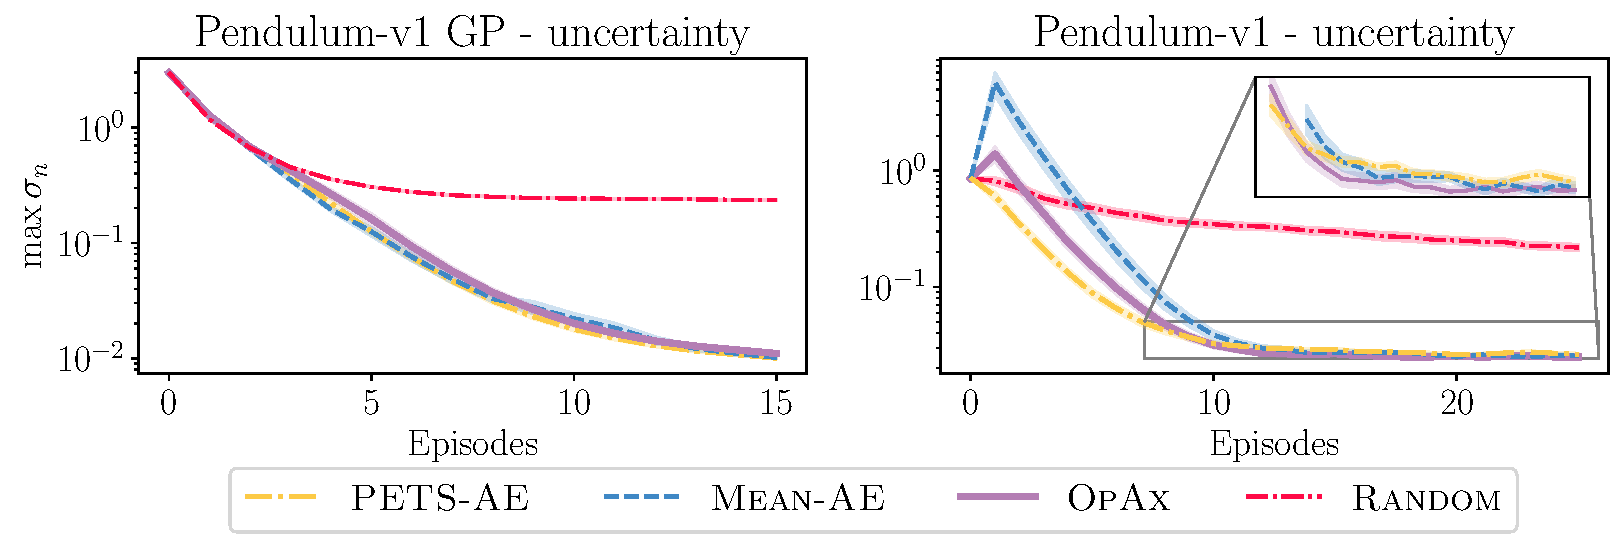
\includegraphics[width=0.75\textwidth]{figures/uncertainty_plotvalidation_eps_std_max.pdf}
    \caption{\looseness -1 Reduction in maximum epistemic uncertainty in \emph{reachable} state-action space for the Pendulum-v1 environment over 10 different random seeds. We evaluate \opacex with both GPs and PE and plot the mean performance with two standard error confidence intervals. For both, active exploration reduces epistemic uncertainty faster compared to random exploration. All active exploration baselines perform well for the GP case, whereas for the PE case \opacex gives slightly lower uncertainties.}
    \label{fig:epistemic_uncertainty_figure}
    %\vspace{-0.5cm}
\end{figure}
\begin{figure}[ht]
%\vspace{-0.2cm}
    \centering
    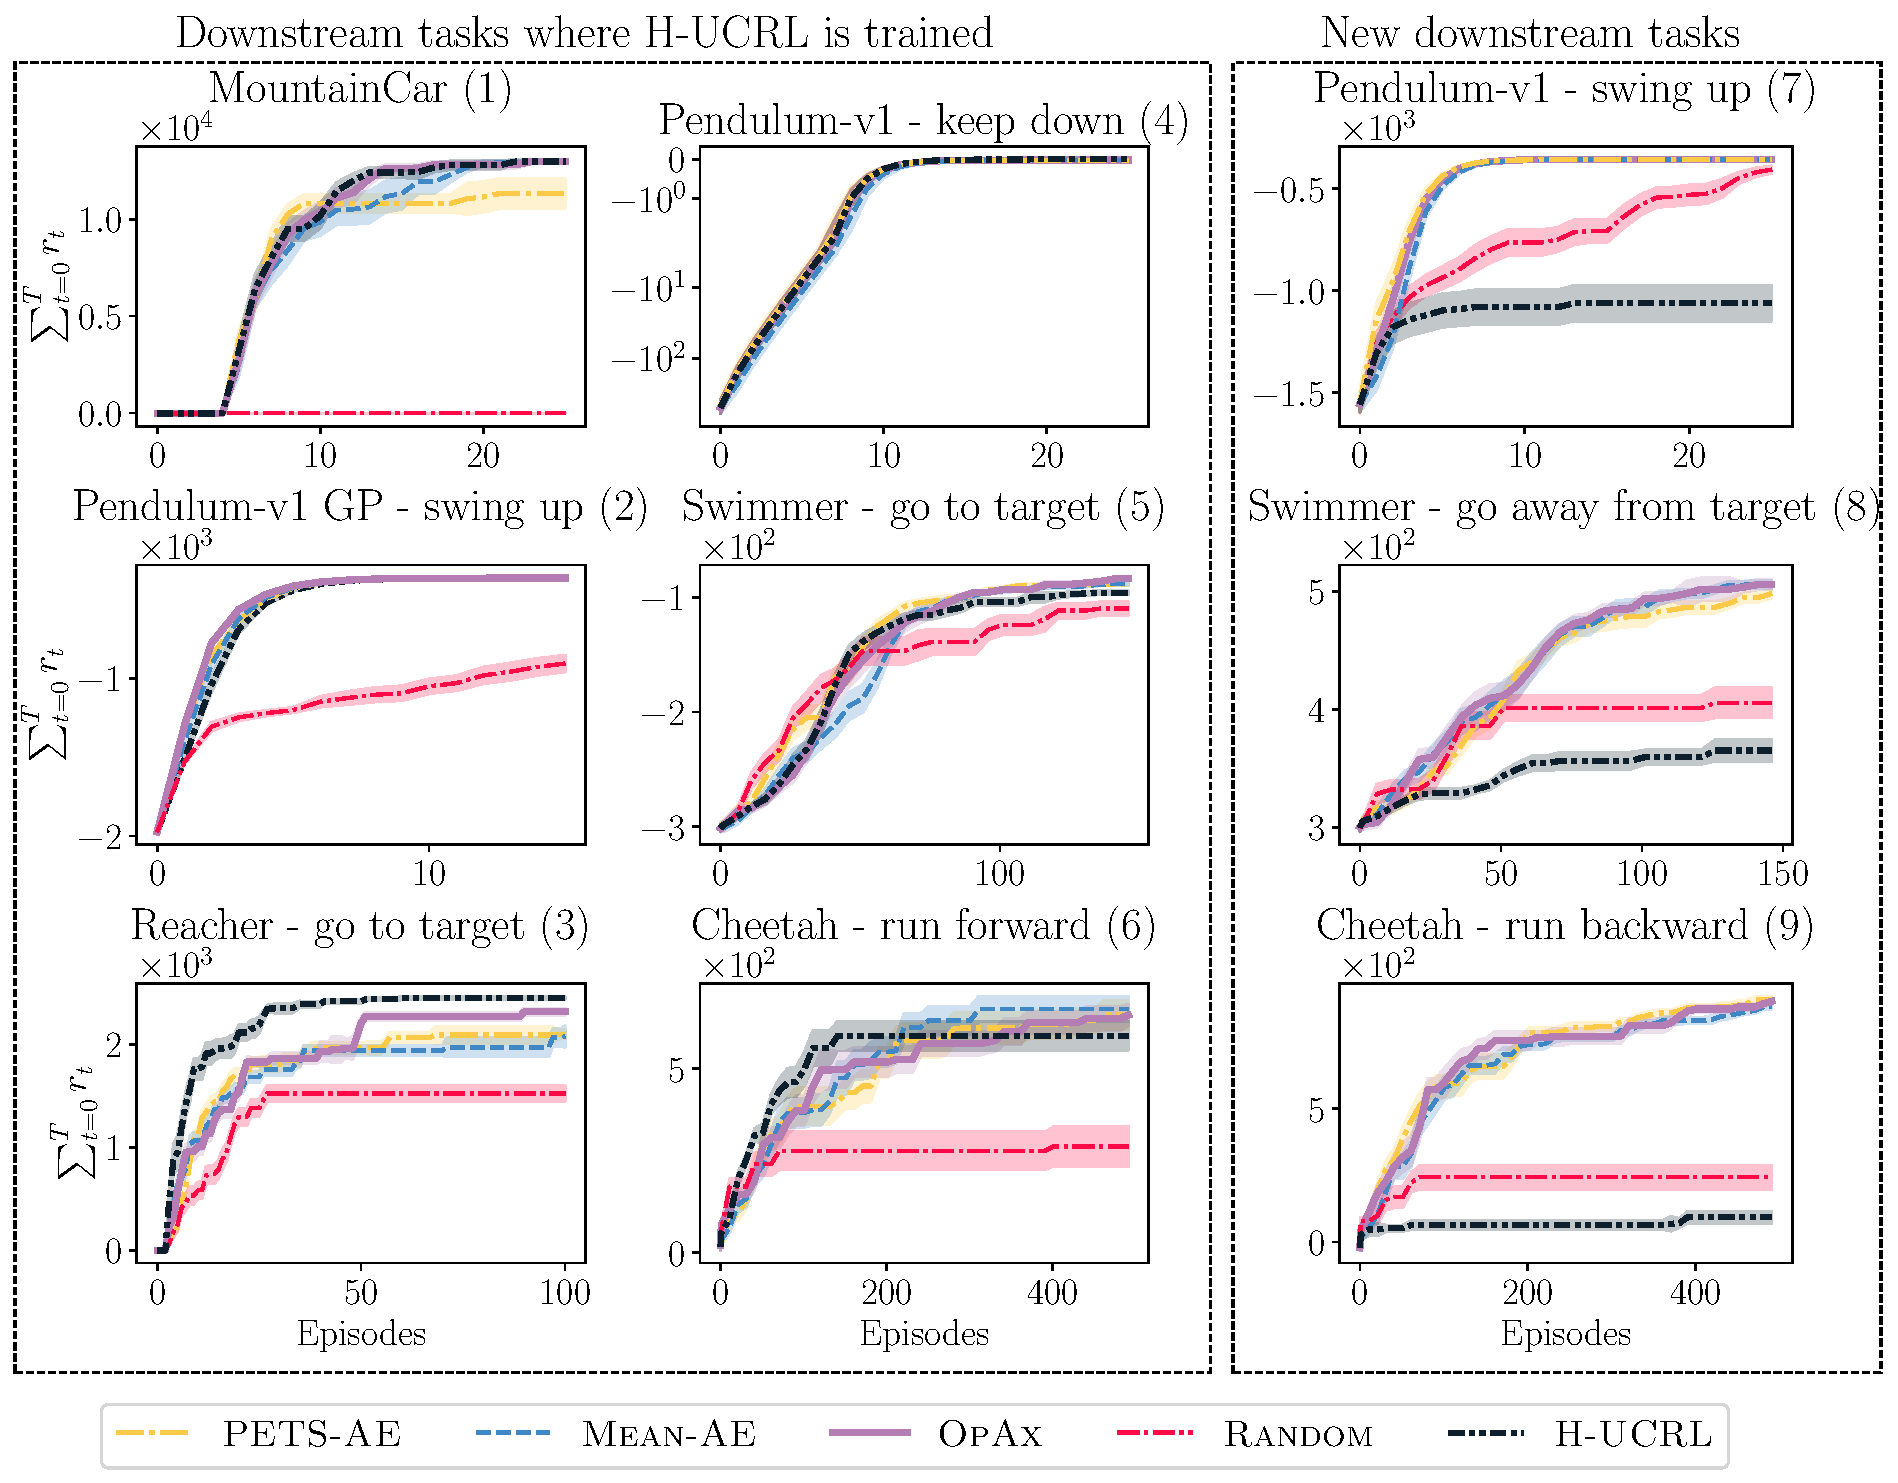
\includegraphics[width=1\textwidth]{figures/results_plot_with_hucrlreward_task_1.pdf}
    \caption{\capt{\looseness-1 We evaluate the downstream performance of our agents over 10 different random seeds and plot the mean performance with two standard error confidence intervals.
    For all the environments we use PE as models, except plot (1), for which we use a GP model (see plot (2) in the figure above). For tasks (1)-(6), we also train \textsc{H-UCRL}, a model-based RL algorithm. Tasks (7)-(9) are new/unseen for \textsc{H-UCRL}. From the Figure, we conclude that (\emph{i}) compared to other active exploration baselines, \opacex constantly performs well and is on par with \textsc{H-UCRL}, and (\emph{ii}) on the new/unseen tasks the active exploration baselines and \opacex outperform \textsc{H-UCRL} by a large margin.
    }}
%\vspace{-0.3cm}
    \label{fig:results_figure}
\end{figure}
%\vspace{-0.1cm}

\paragraph{How fast does active exploration reduce the epistemic uncertainty?}
For this experiment, we consider the Pendulum-v1 environment. We sample transitions at random from the pendulum's \emph{reachable} state-action space and evaluate our model's epistemic uncertainty for varying episodes and baselines. We model the dynamics with both GPs and PE. We depict the result
in \Cref{fig:epistemic_uncertainty_figure}. We conclude that the \textsc{Random} agent is slower in reducing the uncertainty compared to other active exploration methods for both GP and PE models. In particular, from the experiment, we empirically validate \Cref{thm:gp_theorem} for the GP case and also conclude that empirically even when using PE models, we find convergence of epistemic uncertainty. Moreover, we notice for the PE case 
that \opacex reaches smaller uncertainties slightly faster than \textsc{Mean-AE} and \textsc{PETS-AE}. We believe this is due to the additional exploration induced by the optimistic planner. 


%\vspace{-0.1cm}
\paragraph{Can the model learnt through \opacex solve downstream tasks?}
\looseness=-1
We use \opacex and other active exploration baselines to actively learn a dynamics model and then evaluate the learned model on downstream tasks. We consider several tasks, (\emph{i}) Pendulum-v1 swing up, (\emph{ii})  Pendulum-v1 keep down (keep the pendulum at the stable equilibria), (\emph{iii}) MountainCar, (\emph{iv}) Reacher - go to target, (\emph{v}) Swimmer - go to target, 
(\emph{vi}) Swimmer - go away from target (quickly go away from the target position), 
(\emph{vii}) Cheetah - run forward, (\emph{viii}) Cheetah - run backward. For all tasks, we consider PEs, except for (\emph{i}) where we also use GPs. Furthermore,
for the MountainCar and Reacher, we give a reward once the goal is reached. Since this requires long-term planning, we use a SAC policy for these tasks. We use MPC with iCEM for the remaining tasks. We also train \textsc{H-UCRL} on tasks (\emph{i}) with GPs, and (\emph{ii}), (\emph{iii}), (\emph{iv}), (\emph{v}), (\emph{vii}) with PEs. We report the best performance across all episodes. 
%(\emph{i}) MountainCar, (\emph{ii}) Reacher - go to target, where we ask the Reacher's end-effector to reach a desired goal, (\emph{iii}) Swimmer - go to target, here the goal is for the Swimmer to move towards a target, and (\emph{iv}) Cheetah - run forward, where we give positive reward for the Cheetah's forward velocity. For the MountainCar and Reacher tasks, we only give a positive reward if the goal is reached. Since this requires long-term planning, we use a SAC policy for these tasks. We use MPC with iCEM for the remaining tasks. 

To make a fair comparison, we use the following evaluation procedure; first, we perform active exploration for each episode on the environment, and then after every few episodes we use the mean estimate $\vmu_n$ to evaluate our learned model on the downstream tasks. 

\looseness=-1
\Cref{fig:results_figure} shows that all active exploration variants perform considerably better than the \textsc{Random} agent. In particular, for the MountainCar, the \textsc{Random} agent is not able to solve the task. Moreover, \textsc{PETS-AE} performs slightly worse than the other exploration baselines in this environment.
In general, we notice that \opacex always performs well and is able to achieve \textsc{H-UCRL}'s performance on all the tasks for which \textsc{H-UCRL} is trained. 
However, on tasks that are new/unseen for \textsc{H-UCRL}, active exploration algorithms outperform \textsc{H-UCRL}. 
From this experiment, we conclude two things 
(\emph{1}) apart from providing theoretical guarantees, the model learned through \opacex 
also performs well in downstream tasks, and (\emph{2}) active exploration agents generalize well to downstream tasks, whereas \textsc{H-UCRL} performs considerably worse on new/unseen tasks.
We believe this is because, unlike active exploration agents, task-specific model-based RL agents only explore the regions of the state-action space that are relevant to the task at hand.

%\vspace{-0.1cm}
\paragraph{Does \opacex scale to high-dimensional and challenging object manipulation tasks?}
\begin{wrapfigure}[13]{r}{0.2\textwidth}
%\vspace{-1.8cm}
    \label{fig:fpp_pic}
    \centering
    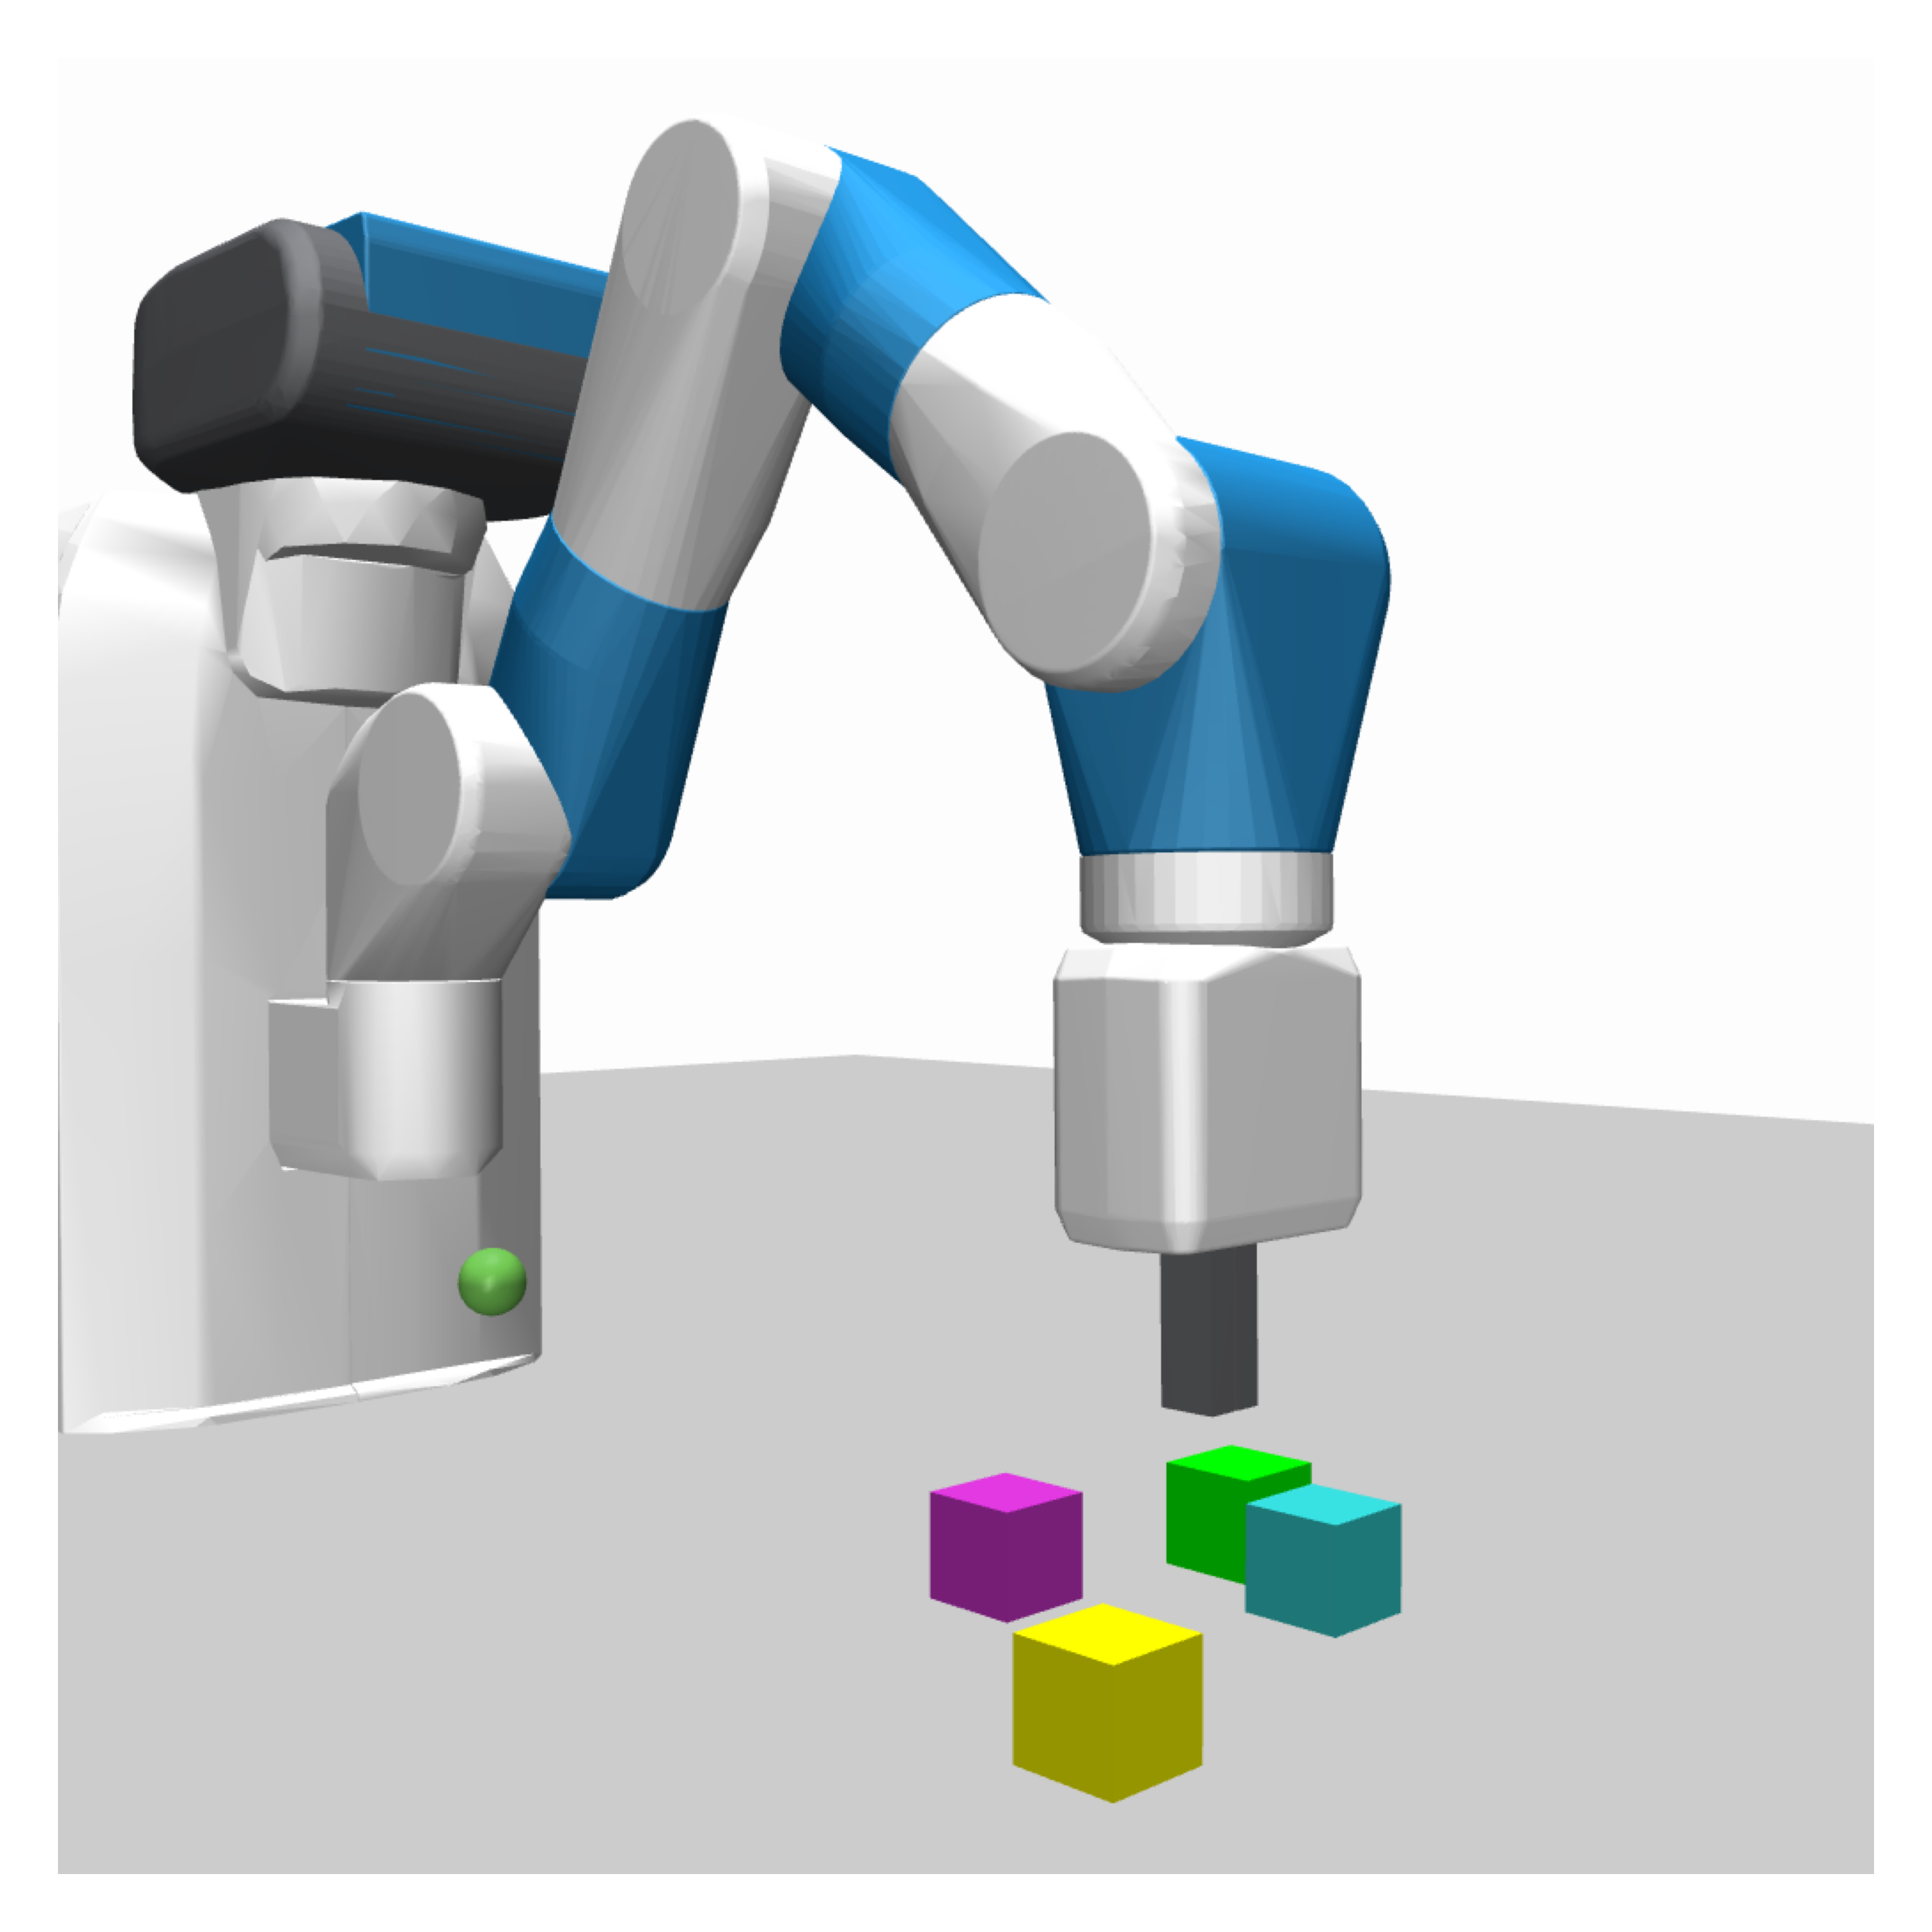
\includegraphics[width=\linewidth]{figures/fpp_construction/env_4obj.png}%\vspace{-.6em}
    \caption{Fetch Pick \& Place Construction environment.}
   % \vspace{-0.6cm}
\setlength{\intextsep}{1.0pt plus 2.0pt minus 2.0pt}
\setlength{\columnsep}{10pt}%
\end{wrapfigure}
To answer this question, we consider the Fetch Pick \& Place Construction environment~\citep{li2020towards}. We again use the active exploration agents to learn a model and then evaluate the success rate of the learned model in three challenging downstream tasks: (\emph{i}) Pick \& Place, (\emph{ii}) Throw, and (\emph{iii}) Flip (see \Cref{fig:construction:success_rates}). The environment contains a \( 7 \)-DoF robot arm and four \( 6 \)-DoF blocks that can be manipulated. In total, the state space is \( 58 \)-dimensional. The \( 4 \)-dimensional actions control the end-effector of the robot in Cartesian space as well as the opening/closing of the gripper. We compare \opacex to \textsc{PETS-AE}, \textsc{Mean-AE}, a random policy as well as \ceeus~\citep{Sancaktaretal22}. \ceeus is a model-based active exploration algorithm, for which \cite{Sancaktaretal22} reports state-of-the-art performance compared to several other active exploration methods. In all three tasks, \opacex is at least on par with the best-performing baselines, including \ceeus.
% Accordingly, we compare our active exploration methods to \ceeus. 
We run \opacex and all baselines with the same architecture and hyperparameter settings. See \Cref{sec:experiment_details} for more details. \looseness -1
%Only the particle sampling during model rollouts in the free-play phase is different between the methods
%: Where \ceeus uses the sampling method denoted as TS$\infty$ in \cite{chua2018pets}, \opacex uses a practical variant of \Cref{algorithm:episodicOpAcEx} 
%(c.f., \Cref{sec:experiment_details} for more details). Plots showing the interaction times in the free-play phase can be found in \Cref{sec:experiment_details}. %\Cref{fig:construction:interaction_times} shows the interaction times for \opacex and \ceeus during the free-play phase in which the algorithms actively gather experience in order to reduce model uncertainties. In each metric \opacex is on par with or has slightly more interaction time than \ceeus except for the interaction time with objects in the air which can be explained by the fact that once the robot lifts an object into the air, the object's movement is fully determined by the movement of the robot resulting in no uncertainty about the object's location.
\begin{figure}[ht]
    \centering
    \begin{subfigure}{.32\linewidth}
        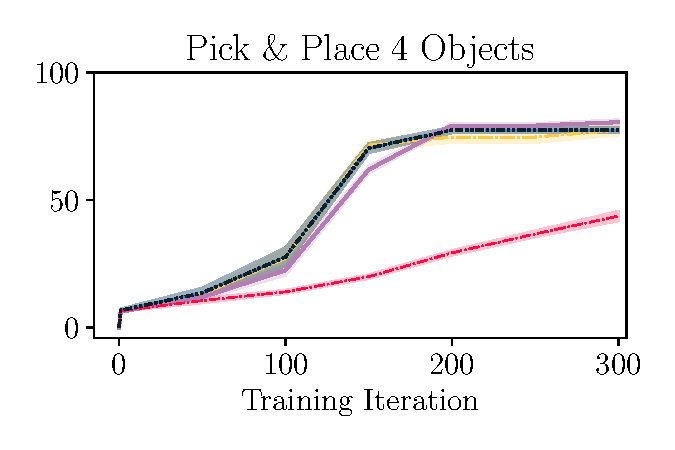
\includegraphics[width=\linewidth]{figures/fpp_construction/construction_pp4_success_monotonous.pdf}
        %\caption{Pick \& Place 4}
    \end{subfigure}
    \begin{subfigure}{.32\linewidth}
        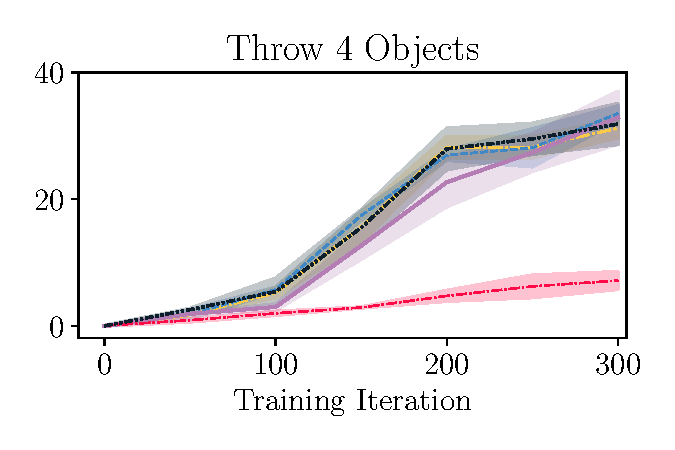
\includegraphics[width=\linewidth]{figures/fpp_construction/construction_throw4_success_monotonous.pdf}
        %\caption{Throw 4}
    \end{subfigure}
    \begin{subfigure}{.32\linewidth}
        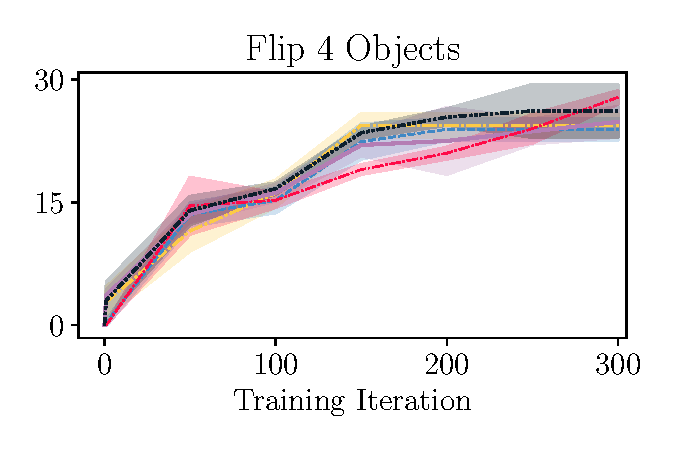
\includegraphics[width=\linewidth]{figures/fpp_construction/construction_flip4_success_monotonous.pdf}
        %\caption{Flip 4}
    \end{subfigure}\\
    
\includegraphics[width=.8\linewidth]{figures/fpp_construction/legend_updated.pdf}
    \caption{\looseness-1 Success rates for pick \& place, throwing and flipping tasks with four objects in the Fetch Pick \& Place Construction environment for \opacex and baselines. \capt{We evaluate task performance via planning zero-shot with models learned using different exploration strategies. We report performance on three independent seeds. \opacex is on par with the best-performing baselines in all tasks.}}
    \label{fig:construction:success_rates}
%\vspace{-0.5cm}
\end{figure}
%\vspace{-0.3cm}
\section{Related Work} \label{sec:related_works}
%\vspace{-0.3cm}
System identification is a broadly studied topic~\citep {ASTROMSystemID, schoukens, SCHON201139, ziemann2022single, ziemann2022learning}. However, system identification from the perspective of experiment design for nonlinear systems is much less understood~\citep{chiuso2019system}. Most methods formulate the identification task through the maximization of intrinsic rewards.
 %Intrinsic rewards depend on the RL agent's model of the system and encourage exploration by suggesting policies that visit transitions where the learned model has less ``information''. 
Common choices of intrinsic rewards are (\emph{i}) model prediction error or ``Curiosity''~\citep{schmidhuber1991possibility, pathak2017curiosity}, (\emph{ii}) novelty of transitions~\citep{stadie2015incentivizing}, and  (\emph{iii}) diversity of skills~\citep{eysenbach2018diversity}.
%. Curiosity approaches encourage collecting data where the learned model makes the most prediction error. Thus, the model error is used as a proxy for lack of information. However, these methods ...
%Alternatively, methods with state visitation count as the intrinsic reward encourage visiting states with low visitation frequency, that is the states that have been less frequently observed by the agent. For finite MDPs 

A popular choice for intrinsic rewards is mutual information or entropy~\citep{learning_and_control_using_gps, active_learning_gp, max, pathak2019self, sekar2020planning}. \cite{learning_and_control_using_gps} propose an
approach to maximize the information gain greedily wrt the immediate next transition, i.e., one-step greedy, whereas \cite{active_learning_gp} consider planning full trajectories.
\cite{max, pathak2019self, sekar2020planning} and \cite{Sancaktaretal22} consider general Bayesian models, such as BNNs, to represent a probabilistic distribution for the learned model. 
\cite{max} propose using the information gain of the model with respect to observed transition as the intrinsic reward. %Accordingly, the algorithm suggests policies that visit transitions which give more information for the learned model. 
To this end, they learn an ensemble of Gaussian neural networks and represent the distribution over models with a Gaussian mixture model (GMM). A similar approach is also proposed in \cite{pathak2019self, sekar2020planning, Sancaktaretal22}. The main difference between \cite{max} and \cite{pathak2019self} lies in how they represent mutual information. Moreover, \cite{pathak2019self} use the model's epistemic uncertainty, that is the disagreement between the ensemble models as an intrinsic reward. \cite{sekar2020planning} link the model disagreement (epistemic uncertainty) reward to maximizing mutual information and demonstrate state-of-the-art performance on several high-dimensional tasks. 
Similarly, \cite{Sancaktaretal22}, use the disagreement in predicted trajectories of an ensemble of neural networks to direct exploration. Since trajectories can diverge due to many factors beyond just the model epistemic uncertainty, e.g., aleatoric noise, this approach is restricted to deterministic systems and susceptible to systems with unstable equilibria. 
Our approach is the most similar to \cite{pathak2019self, sekar2020planning} since we also propose the model epistemic uncertainty as the intrinsic reward for planning. However, we thoroughly and theoretically motivate this choice of reward from a Bayesian experiment design perspective. Furthermore,
we induce additional exploration in \opacex through our optimistic planner and rigorously study the theoretical properties of the proposed methods. On the contrary, most of the prior work discussed above either uses the mean planner (\textsc{Mean-AE}) or does not discuss the planner thoroughly or provide any theoretical results. In general, theoretical guarantees for active exploration algorithms are rather immature~\citep{chakraborty2023steering, wagenmaker2023optimal} and mostly restrictive to a small class of systems~\citep{simchowitz2018learning, tarbouriech2020active, wagenmaker2020active, mania2020active}. %In this work, we derive an upper bound on the information gain for \opacex for well-calibrated models. In addition, for the GP case, we show convergence for a rich class of RKHS, i.e.,  we show that information gain goes to zero. 
To the best of our knowledge, we are the first to give convergence guarantees for a rich class of nonlinear systems.

\looseness=-1
While our work focuses on the active learning of dynamics, there are numerous works that study exploration in the context of reward-free RL \citep{jin2020reward, kaufmann2021adaptive, wagenmaker2022reward, chen2022statistical}. However, most methods in this setting give guarantees for special classes of MDPs~\citep{jin2020reward, kaufmann2021adaptive, wagenmaker2022reward, qiu2021reward, chen2022statistical} and result in practical algorithms. On the contrary, we focus on solely learning the dynamics. While a good dynamics model may be used for zero-shot planning, it also exhibits more relevant knowledge about the system such as its stability or sensitivity to external effects. Furthermore, our proposed method is not only theoretically sound but also practical. 
%Another approach is proposed by
%\cite{Sancaktaretal22}, where the disagreement in predicted trajectories of an ensemble of neural networks is used to direct exploration. Moreover, instead of using intrinsic rewards for policy optimization, \cite{Sancaktaretal22} use the iCEM black box optimizer~\citep{iCem}
%to suggest actions that maximize disagreement in model trajectories. However, the approach is restricted to deterministic systems and susceptible to systems with unstable equilibria. In particular, for systems with unstable equilibria, small uncertainties around the equilibrium, can lead to drastic disagreement in trajectories. Accordingly, the algorithm might suggest policies that visit the unstable equilibrium even if the dynamics are accurate around that region. 
%\vspace{-0.4cm}
\section{Conclusion}
%\vspace{-0.3cm}
\looseness=-1
We present \opacex, a novel model-based RL algorithm for the active exploration of unknown dynamical systems. Taking inspiration from Bayesian experiment design, we provide a comprehensive explanation for using model epistemic uncertainty as an intrinsic reward for exploration. 
By leveraging the \emph{optimistic in the face of uncertainty} paradigm, we put forth first-of-their-kind theoretical results on the convergence of active exploration agents in reinforcement learning. Specifically, we study convergence properties of general Bayesian models, such as BNNs. For the frequentist case of RKHS dynamics, we established sample complexity bounds and convergence guarantees for \opacex for a rich class of functions.
 We evaluate the efficacy of \opacex across various RL environments with state space dimensions from two to 58. The empirical results corroborate our theoretical findings, as \opacex displays systematic and effective exploration across all tested environments and exhibits strong performance in zero-shot planning for new downstream tasks.
%We propose \opacex a state-of-the-art model-based RL algorithm for active exploration of dynamical systems. Inspired by Bayesian experiment design, we thoroughly motivate using the model epistemic uncertainty as an intrinsic reward for active exploration. Furthermore, we use an \emph{optimistic paradigm} to induce further exploration in \opacex. We provide first-of-its-kind theoretical results for the convergence of active exploration agents in RL.
%Moreover, we study the convergence properties for general Bayesian models such as BNNs, and for the frequentist setting with GP models, we provide sample complexity bound and convergence guarantees for \opacex for a rich class of functions.
%We evaluate \opacex on several RL environments with state space dimensions ranging from two to 58. Our experiments validate the theoretical results and show that \opacex systematically explores well for all the environments and performs well for zero-shot planning on novel downstream tasks.
\clearpage
\begin{ack}
We would like to thank Jonas H\"ubotter for the insightful discussions and his feedback on this work. Furthermore, we also thank Alex Hägele, 
Parnian Kassraie, Scott Sussex, and Dominik Baumann for their feedback. 

This project has received funding from the Swiss National Science Foundation under NCCR Automation, grant agreement 51NF40 180545, and the Microsoft Swiss Joint Research Center.

\end{ack}


%\newpage

\bibliographystyle{apalike}
\bibliography{refs}




\newpage
\appendix

\renewcommand*\contentsname{Contents of Appendix}
\etocdepthtag.toc{mtappendix}
\etocsettagdepth{mtchapter}{none}
\etocsettagdepth{mtappendix}{subsection}
\tableofcontents

\newpage
\section{Proofs for \cref{sec:theoretical_results}} \label{sec:proofs}
We first prove some key properties of our active exploration objective in \Cref{eq:exploration_op}. Then, we prove \Cref{thm:main_theorem} which holds for general Bayesian models, and finally we prove \Cref{thm:gp_theorem}, which guarantees convergence for the frequentist setting where the dynamics are modeled using a GP. 
\begin{lemma}[Properties of \opacex's objective]
\label{cor:bounded_objective}
Let \Cref{assumption: Well Calibration Assumption} and \ref{ass:lipschitz_continuity} hold, then the following is true for all $n\geq 0$,
\begin{align*}
     \log \left(1 + \frac{\sigma_{n-1, j}^2(\vx_t, \vpi(\vx_t))}{\sigma^2}\right) &\ge 0 \tag{1} \\
     \frac{1}{2}\sup_{\vpi \in \Pi, \veta \in \Xi} \hspace{0.2em} \E\left[\left(\sum_{t=0}^{T-1} \sum^{d_x}_{j=1} \log \left(1 + \frac{\sigma_{n-1, j}^2(\vx_t, \vpi(\vx_t))}{\sigma^2}\right)\right)^2\right] &\leq \frac{1}{2} T^2 d^2_x \log^2 \left(1 + \frac{\sigma^2_{\max}}{\sigma^2}\right) \tag{2}, \\
      \left\vert \frac{1}{2}\sum^{d_x}_{j=1} \log \left(1 + \frac{\sigma_{n, j}^2(\vz)}{\sigma^{2}}\right) - \log \left(1 + \frac{\sigma_{n, j}^2(\vz')}{\sigma^{2}}\right) \right\vert &\leq \frac{d_x\sigma_{\max} L_{\vsigma}}{\sigma^2} \norm{\vz - \vz'} \tag{3}.
\end{align*}
where $\sigma_{\max} = \sup_{\vz \in \setZ; i \geq 0; 1\leq j\leq d_x} \sigma_{i, j}(\vz)$.
\end{lemma}
\begin{proof}
    The positivity of the reward follows from the positive definiteness of the epistemic uncertainty $\sigma_{n-1, j}$. For (2), the following holds
    \begin{align*}
        &\E\left[\left(\sum_{t=0}^{T-1} \sum^{d_x}_{j=1} \log \left(1 + \frac{\sigma_{n-1, j}^2(\vx_t, \vpi(\vx_t))}{\sigma^2}\right)\right)^2\right] \\
        &\leq  \E\left[\sum_{t=0}^{T-1} \sum^{d_x}_{j=1} T d_x \log^2 \left(1 + \frac{\sigma_{n-1, j}^2(\vx_t, \vpi(\vx_t))}{\sigma^2}\right)\right] \\
        &\leq \E\left[\left(\sum_{t=0}^{T-1} \sum^{d_x}_{j=1} T d_x \log^2 \left(1 + \frac{\sigma^2_{\max}}{\sigma^2}\right)\right)\right] \\
        &\leq T^2 d^2_x \log^2 \left(1 + \frac{\sigma^2_{\max}}{\sigma^2}\right)
    \end{align*}
    From hereon, let $J_{\max} = \sfrac{1}{2} T^2 d^2_x \log^2 \left(1 + \sigma^{-2}\sigma^2_{\max}\right)$.
    
      Finally, we show that this reward is Lipschitz continuous. 
    \begin{align*}
        \lvert\sigma^2_{n, j}(\vz)  -  \sigma^2_{n, j}(\vz')\rvert &= 
         \vert\sigma_{n, j}(\vz)  \sigma_{n, j}(\vz) -  \sigma_{n, j}(\vz)\sigma_{n, j}(\vz') + \sigma_{n, j}(\vz)\sigma_{n, j}(\vz') - \sigma_{n, j}(\vz')  \sigma_{n, j}(\vz')\rvert \\
         &\leq L_{\sigma}\norm{\vz - \vz'} \sigma_{n, j}(\vz) +  L_{\sigma}\norm{\vz - \vz'} \sigma_{n, j}(\vz') \\
         &\leq 2\sigma_{\max}L_{\sigma}\norm{\vz - \vz'}.
    \end{align*}
    \begin{align*}
            \left\vert \frac{1}{2}\sum^{d_x}_{j=1} \log \left(1 + \frac{\sigma_{n, j}^2(\vz)}{\sigma^{2}}\right) - \log \left(1 + \frac{\sigma_{n, j}^2(\vz')}{\sigma^{2}}\right) \right\vert
            &= \frac{1}{2}\left\vert \sum^{d_x}_{j=1} \log\left(1+\frac{
            \frac{\sigma^2_{n, j}(\vz) - \sigma^2_{n, j}(\vz') }{\sigma^2}
            }{1 + \frac{\sigma^2_{n, j}(\vz')}{\sigma^2}}\right)\right\vert \\
            &\leq \frac{1}{2} \left\vert \sum^{d_x}_{j=1} \log\left(1+
            \frac{\mid\sigma^2_{n, j}(\vz) - \sigma^2_{n, j}(\vz') \mid}{\sigma^2}\right)\right\vert \\
            &\leq \frac{1}{2 \sigma^2} \sum^{d_x}_{j=1} \left\vert\sigma^2_{n, j}(\vz) - 
            \sigma^2_{n, j}(\vz')\right\vert \tag{*}\\
            &\leq \frac{d_x\sigma_{\max} L_{\vsigma}}{\sigma^2} \norm{\vz - \vz'}.
\end{align*}
Where (*) is true because for all $x\geq 0$, $\log(1 + x) \leq x$.
\end{proof}
 %and $J_{n, t}(\vx_{t}, \vpi, \veta)$ the $T-t$ step cost-to-go from $\vx_{t}$ onwards under the policy $\vpi$ and dynamics induced by $\veta$ at iteration $n$.

\begin{corollary}[\opacex gives an optimistic estimate on \Cref{eq:exploration_op}]
Let \Cref{assumption: Well Calibration Assumption} hold 
 and $\vpi_n^{*}$ denote the solution to \Cref{eq:exploration_op} and $J_n(\vpi_n^*)$ the resulting objective. Similarly, let $\vpi_n$ and $\veta_n$ be the solution to \Cref{eq:exploration_op_optimistic} and $J_n(\vpi_n, \veta_n)$ the corresponding value of the objective. Then with probability at least $1-\delta$ we have for every episode $n \in \set{1, \ldots, N}$:
\begin{equation*}
    J_n(\vpi_n^*) \le J_n(\vpi_n, \veta_n).
\end{equation*}
\label{cor:optimistic_estimate}
\end{corollary}
\begin{proof}
    Follows directly from \Cref{assumption: Well Calibration Assumption}.
\end{proof}

\subsection{Proof of \Cref{lem:optimistic_planning_regret}}
\begin{lemma}[Difference in Policy performance]
Let $J_{r, k}(\vpi, \vx_k) =  \E_{\vtau^{\vpi}}\left[\sum_{t=k}^{T-1} r(\vx_t, \vpi(\vx_{t}))\right]$ and $A_{r, k}(\vpi, \vx, \va) =  \E_{\vtau^{\vpi}}\left[r(\vx, \va) + J_{r, k + 1}(\vpi, \vx') - J_{r, k}(\vpi, \vx) \right]$ with $\vx' = \vf^*(\vx, \va) + \vw$. For simplicity we refer to  $J_{r, 0}(\vpi, \vx_0) = J_r (\vpi, \vx_0)$. 
The following holds for all $\vx_0 \in \setX$:
\begin{equation*}
    J_r (\vpi', \vx_0) -  J_r (\vpi, \vx_0) = \E_{\vtau^{\vpi'}} \left[\sum^{T-1}_{t=0} A_{r, t}(\vpi, \vx'_t, \vpi'(\vx'_t))\right]
\end{equation*}
\label{lemma:Difference in policy}
\end{lemma}
\begin{proof}
    \begin{align*}
         J_r (\vpi', \vx_0) &= \E_{\vtau^{\vpi'}} \left[\sum^{T-1}_{t=0} r(\vx'_t, \vpi'(\vx'_t))\right] = \E_{\vtau^{\vpi'}} \left[r(\vx_0, \vpi'(\vx_0)) + J_{r, 1}(\vpi', \vx'_1)\right] \\
         &= \E_{\vtau^{\vpi'}}  \left[r(\vx_0, \vpi'(\vx_0)) + J_{r, 1}(\vpi, \vx'_1) + J_{r, 1}(\vpi', \vx'_1) - J_{r, 1}(\vpi, \vx'_1)\right] \\
         &= \E_{\vtau^{\vpi'}}  \left[r(\vx_0, \vpi'(\vx_0)) + J_{r, 1}(\vpi, \vx'_1) - J_r(\vpi, \vx_0)\right] \\
         &+ J_r(\vpi, \vx_0) + \E_{\vtau^{\vpi'}}  \left[J_{r, 1}(\vpi', \vx'_1) - J_{r, 1}(\vpi, \vx'_1)\right] \\
        &= \E_{\vtau^{\vpi'}}  \left[A_{r, 0}(\vpi, \vx_0, \vpi'(\vx_0))\right] + J_r(\vpi, \vx_0) + \E_{\vtau^{\vpi'}}  \left[J_{r, 1}(\vpi', \vx_1) - J_{r, 1}(\vpi, \vx_1)\right]
    \end{align*}
    Therefore we obtain
    \begin{equation*}
        J_r (\vpi', \vx_0) - J_r(\vpi, \vx_0) = \E_{\vtau^{\vpi'}}  \left[A_0(\vpi, \vx_0, \vpi'(\vx_0))\right] +  \E_{\vtau^{\vpi'}}  \left[J_{r, 1}(\vpi', \vx'_1) - J_{r, 1}(\vpi, \vx'_1)\right].
    \end{equation*}
    Using the same argument for $J_{r, 1}$, $J_{r, 2}$, \dots, $J_{r, T-1}$ and that $J_{r, T}(\vpi, \vx) = 0$ for all $\vpi \in \Pi$ and $\vx \in \setX$ completes the proof.
\end{proof}
Assume a policy $\vpi$ is fixed and dynamics are of the form:
\begin{equation}
    \vx' = \vmu_n(\vx, \vpi(\vx)) + \beta_n(\delta) \vsigma(\vx, \vpi(\vx))\vu + \vw.
\end{equation}
Here $\vu \in [-1, 1]^{d_x}$. Furthermore, assume that the associated running rewards do not depend on $\vu$, that is, $r(\vx_t)$, and let $\veta \in \Xi$ denote the policy, i.e., $\veta: \setX \to [-1, 1]^{d_x}$.
\begin{corollary}
The following holds for all $\vx_0 \in \setX$ and policy $\vpi$:
\begin{equation*}
    J_r (\vpi, \veta', \vx_0) -  J_r (\vpi, \veta, \vx_0) = \E_{\vtau^{\veta'}}  \left[\sum^{T-1}_{t=0} J_{r, t+1}(\vpi, \veta, \vx'_{t+1}) -  J_{r, t+1}(\vpi, \veta, \vx_{t+1})\right],
\end{equation*}
with $\vx_{t+1} = \vmu_n(\vx'_t, \vpi(\vx'_t)) + \beta_n(\delta) \vsigma(\vx'_t, \vpi(\vx'_t))\veta(\vx'_t) + \vw_t$, and $\vx'_{t+1} = \vmu_n(\vx'_t, \vpi(\vx'_t)) + \beta_n(\delta) \vsigma(\vx'_t, \vpi(\vx'_t))\veta'(\vx'_t) + \vw_t$.
\label{cor:Difference in hallucinated policy}
\end{corollary}
\begin{proof}
    From \Cref{lemma:Difference in policy} we have
    \begin{equation*}
    J_r (\vpi, \veta', \vx_0) -  J_r (\vpi, \veta, \vx_0) = \E_{\vtau^{\veta'}}  \left[\sum^{T-1}_{t=0} A_{r, t}(\veta, \vx'_{t}, \veta'(\vx'_t))\right].
\end{equation*}
Furthermore, 
\begin{align*}
    \E_{\vtau^{\veta'}}\left[A_{r, t}(\veta, \vx'_{t}, \veta'(\vx'_t))\right] &= \E_{\vtau^{\veta'}} \left[r(\vx'_t) + J_{r, t+1}(\vpi, \veta, \vx'_{t+1}) - J_{r, t}(\vpi, \veta, \vx'_{t})\right] \\
    &= \E_{\vtau^{\veta'}} \left[r(\vx'_t) + J_{r, t+1}(\vpi, \veta, \vx'_{t+1}) - r(\vx'_t) - J_{r, t+1}(\vpi, \veta, \vx_{t+1})\right] \\
    &= \E_{\vtau^{\veta'}}\left[J_{r, t+1}(\vpi, \veta, \vx'_{t+1}) - J_{r, t+1}(\vpi, \veta, \vx_{t+1})\right].
\end{align*}
\end{proof}
\begin{proof}[Proof of \Cref{lem:optimistic_planning_regret}]
From \Cref{assumption: Well Calibration Assumption} we know that with probability at least $1-\delta$ there exists a $\Bar{\veta}$ such that $\vf^*(\vz) = \vmu_n(\vz) + \beta_n(\delta) \vsigma(\vz)\Bar{\veta}(\vx)$ for all $\vz \in \setZ$.
\begin{align*}
     J_n(\vpi_n^*) - J_n(\vpi_n) &\leq J_n(\vpi_n, \veta_n) - J_n(\vpi_n) \tag{\Cref{cor:optimistic_estimate}}\\
     &= J_n(\vpi_n, \veta_n) - J_n(\vpi_n, \Bar{\veta})\\
     &= \E_{\vtau^{\Bar{\veta}}} \left[\sum^{T-1}_{t=0} J_{n, t+1}(\vpi_n, \veta_n, \vx'_{t+1}) -  J_{n, t+1}(\vpi_n, \veta_n, \vx_{t+1})\right] \tag{\Cref{cor:Difference in hallucinated policy}}\\
    &= \E_{\vtau^{\vpi_n}}\left[\sum^{T-1}_{t=0} J_{n, t+1}(\vpi_n, \veta_n, \vx'_{t+1}) -  J_{n, t+1}(\vpi_n, \veta_n, \vx_{t+1})\right], \tag{Expectation wrt $\vpi_n$ under true dynamics $\vf^*$}\\
    &\text{with } \vx_{t+1} = \vf^*(\vx_{t}, \vpi_n(\vx_t)) + \vw_t, \\
    &\text{and } \vx'_{t+1} = \vmu_{n-1}(\vx_t, \vpi_n(\vx_t)) + \beta_{n-1}(\delta)\vsigma_{n-1}(\vx_t, \vpi_n(\vx_t)) \veta_n(\vx_t) + \vw_t.
\end{align*}
    
\end{proof}

\subsection{Analyzing regret of optimistic planning}
In the following, we analyze the regret of optimistic planning for both $\sigma$-Gaussian noise and $\sigma$-sub Gaussian noise case. We start with the Gaussian case.
\begin{lemma}[Absolute expectation Difference Under Two Gaussians (Lemma C.2.~\cite{kakade2020information})]
\label{lem:absolute_diff_gaussians}
For Gaussian distribution $\setN(\mu_1, \sigma^2 \mathbb{I})$ and $\setN(\mu_2, \sigma^2 \mathbb{I})$, and for any (appropriately measurable) positive function $g$, it holds that:
\begin{equation*}
    \left\lvert \E_{z \sim \setN_1}[g(z)] - \E_{z \sim \setN_2}[g(z)] \right\rvert \leq \min\left\{ \frac{\norm{\mu_1 - \mu_2}}{\sigma^2}, 1 \right\} \sqrt{\E_{z \sim \setN_1}[g^2(z)]}
\end{equation*}
\end{lemma}
\begin{proof}
    \begin{align*}
        \left\lvert \E_{z \sim \setN_1}[g(z)] - \E_{z \sim \setN_2}[g(z)] \right\rvert &= \left\lvert \E_{z \sim \setN_1} \left[ g(z) \left(1-\frac{\setN_{2}}{\setN_1}\right)\right]\right\rvert \\
        &\leq \left\lvert \sqrt{\E_{z \sim \setN_1} \left[ g^2(z)\right]} \sqrt{\E_{z \sim \setN_1}\left[\left(1-\frac{\setN_{2}}{\setN_1}\right)^2\right]}\right\rvert \\
        &= \sqrt{\E_{z \sim \setN_1} \left[ g^2(z)\right]} \sqrt{\E_{z \sim \setN_1}\left[\left(1-\frac{\setN_{2}}{\setN_1}\right)^2\right]} \\
        &\leq \sqrt{\E_{z \sim \setN_1}[g^2(z)]} \min\left\{ \frac{\norm{\mu_1 - \mu_2}}{\sigma^2}, 1 \right\} \tag{Lemma C.2.~\cite{kakade2020information}}
    \end{align*}
\end{proof}

\begin{corollary}[Regret of optimistic planning for Gaussian noise]
     Let $\vpi^*_n$, $\vpi_n$ denote the solution to \Cref{eq:exploration_op} and \Cref{eq:exploration_op_optimistic} 
 respectively, and $\vz^*_{n, t}$, $\vz_{n, t}$ the corresponding state-action pairs visited during their respective trajectories. Furthermore, let \Cref{assumption: Well Calibration Assumption} - \ref{ass:noise_properties} hold. Then, the following is true for all $n\geq 0$, $t \in  [0, T-1]$, with probability at least $1-\delta$
 \begin{align*}
     J_n(\vpi_n^*) - J_n(\vpi_n) &\leq \setO\left(T \E_{\vtau^{\vpi_n}} \left[\sum^{T-1}_{t=0} \frac{(1 + \sqrt{d_x}) \beta_{n-1}(\delta) \norm{\vsigma_{n-1}(\vz_{n, t})}}{\sigma^2}\right]\right)
     %\E \left[J_{n, t+1}(\vpi_n, \veta_n, \vx'_{t+1}) -  J_{n, t+1}(\vpi_n, \veta_n, \vx_{t+1})\right] \leq \sqrt{J_{\max}} \min\left\{ \frac{2\beta_n(\delta)\norm{\vsigma_{n-1}(\vz_t)}}{\sigma^2}, 1 \right\}.
 \end{align*}
\label{cor:bounding_diff_in_performance}
\end{corollary}
\begin{proof}
For simplicity, define $g_n(\vx) = J_{n, t+1}(\vpi_n, \veta_n, \vx)$.
Note since $\vw_t \sim \setN(0, \sigma^2 \mathbb{I})$ (\Cref{ass:noise_properties}), we have that $\vx'_{t+1}$ and $\vx_{t+1}$ are also Gaussians. Therefore, we can leverage \Cref{lem:absolute_diff_gaussians}.
\begin{align*}
    \E_{\vtau^{\vpi_n}} &\left[J_{n, t+1}(\vpi_n, \veta_n, \vx'_{t+1}) -  J_{n, t+1}(\vpi_n, \veta_n, \vx_{t+1})\right] = \E \left[g_n(\vx'_{t+1}) -  g_n(\vx_{t+1})\right] \\
    &\le  \sqrt{\E[g_n^2(\vx_{t+1})]} \min\left\{ \frac{\norm{\vx'_{t+1} - \vx_{t+1}}}{\sigma^2}, 1 \right\} \tag{\Cref{lem:absolute_diff_gaussians}} \\
   &\le \sqrt{J_{\max}} \min\left\{ \frac{\norm{\vx'_{t+1} - \vx_{t+1}}}{\sigma^2}, 1 \right\} \tag{\Cref{cor:bounded_objective}}.
\end{align*}
Furthermore, 
\begin{align*}
    \norm{\vx'_{t+1} - \vx_{t+1}} &= \norm{\vmu_{n-1}(\vx_t, \vpi_n(\vx_t)) + \beta_{n-1}(\delta)\vsigma_{n-1}(\vx_t, \vpi_n(\vx_t)) \veta_n(\vx_t) - \vf^*(\vx_t, \vpi_n(\vx_t))} \\
    &\le \norm{\vmu_{n-1}(\vx_t, \vpi_n(\vx_t)) - \vf^*(\vx_t, \vpi_n(\vx_t))} \\
    &+ \beta_{n-1}(\delta) \norm{\vsigma_{n-1}(\vx_t, \vpi_n(\vx_t))}\norm{\veta_n(\vx_t)} \\
    &\le (1 + \sqrt{d_x}) \beta_{n-1}(\delta) \norm{\vsigma_{n-1}(\vx_t, \vpi_n(\vx_t))} \tag{\Cref{assumption: Well Calibration Assumption}}.
\end{align*}
Next, we use \Cref{lem:optimistic_planning_regret} 
\begin{align*}
   J_n(\vpi_n^*) - J_n(\vpi_n)  &\leq  \E_{\vtau^{\vpi_n}} \left[\sum^{T-1}_{t=0} J_{n, t+1}(\vpi_n, \veta_n, \vx'_{t+1}) -  J_{n, t+1}(\vpi_n, \veta_n, \vx_{t+1})\right], \\
   &\leq \E_{\vtau^{\vpi_n}} \left[\sum^{T-1}_{t=0} \sqrt{J_{\max}} \min\left\{ \frac{(1 + \sqrt{d_x}) \beta_{n-1}(\delta) \norm{\vsigma_{n-1}(\vx_t, \vpi_n(\vx_t))}}{\sigma^2}, 1 \right\}\right], \\
   &\leq \sqrt{J_{\max}}  \E_{\vtau^{\vpi_n}} \left[\sum^{T-1}_{t=0} \frac{(1 + \sqrt{d_x}) \beta_{n-1}(\delta) \norm{\vsigma_{n-1}(\vx_t, \vpi_n(\vx_t))}}{\sigma^2}\right], \\
   &= \setO\left(T \E_{\vtau^{\vpi_n}} \left[\sum^{T-1}_{t=0} \frac{(1 + \sqrt{d_x}) \beta_{n-1}(\delta) \norm{\vsigma_{n-1}(\vx_t, \vpi_n(\vx_t))}}{\sigma^2}\right]\right).
\end{align*}

\end{proof}


\begin{lemma}[Regret of planning optimistically for sub-Gaussian noise]
\label{lem:simple_regret_planning}
    Let $\vpi^*_n$, $\vpi_n$ denote the solution to \Cref{eq:exploration_op} and \Cref{eq:exploration_op_optimistic} 
 respectively, and $\vz^*_{n, t}$, $\vz_{n, t}$ the corresponding state-action pairs visited during their respective trajectories. Furthermore, let \Cref{assumption: Well Calibration Assumption} and \ref{ass:lipschitz_continuity} hold, and relax \Cref{ass:noise_properties} to $\sigma$-sub Gaussian noise. Then, the following is true for all $n\geq 0$ with probability at least $1-\delta$
    \begin{equation*}
        J_n(\vpi_n^*) - J_n(\vpi_n) \leq \setO\left(L^{T-1}_{\vsigma} \beta^T_{n-1}(\delta) T \E_{\vtau^{\vpi_n}}\left[\sum^{T-1}_{t=0} \norm{ \vsigma_{n-1, j}(\vz_{n, t})} \right]\right)
    \end{equation*}
\end{lemma}
\begin{proof}
    \citet[Lemma~5]{curi2020efficient} bound the regret with the sum of epistemic uncertainties for Lipschitz continuous reward functions, under \Cref{assumption: Well Calibration Assumption} and~\ref{ass:lipschitz_continuity} for sub-Gaussian noise (c.f., \citet[Theorem 3.5]{rothfuss2023hallucinated} for a more rigorous derivation). For the active exploration setting, the reward in episode $n+1$ is 
    \begin{equation*}
        r(\vz) = \frac{1}{2}\sum^{d_x}_{j=1} \log \left(1 + \frac{\vsigma_{n-1, j}^2(\vz)}{\sigma^{2}}\right).
    \end{equation*}
    We show in \Cref{cor:bounded_objective} that our choice of exploration reward is Lipschitz continuous. Thus, can use the regret bound from \citet{curi2020efficient}.
\end{proof}

Compared to the Gaussian case, $\sigma$-sub Gaussian noise has the additional exponential dependence on the horizon $T$, i.e., the 
$\beta^T_n$ term. This follows from the analysis through Lipschitz continuity. Moreover, as we show in \Cref{lem:optimistic_planning_regret}, the regret of planning optimistically is proportional to the change in value under the same optimistic dynamics and policy, but different initial states. The Lipschitz continuity property of our objective allows us to relate the difference in values to the discrepancy in the trajectories. Even for linear systems, trajectories under the same dynamics and policy but different initial states can deviate exponentially in the horizon. 

\subsection{Proof for general Bayesian models}
In this section, we analyze the information gain for general Bayesian models and prove \Cref{thm:main_theorem}.
% \begin{lemma}\label{lem:monotone_submodular}
%   $F$ from \cref{def:MI} is a monotone submodular function.
% \end{lemma}
% \begin{proof}
% Consider any $\setD \subset \setD'$, and trajectory $\vtau$. Let $\Delta_F(\vtau \mid \setD')  = F(\vtau \cup \setD') - F(\setD')$ denote the difference in mutual information. 
%     \begin{align*}
%         \Delta_F(\vtau \mid \setD') -  \Delta_F(\vtau \mid \setD) &= 
%         H\left(\vy_{\setD' \cup \vtau}\right) - H\left(\vy_{\setD'}\right) - H\left(\vy_{\setD \cup \vtau}\right) + H\left(\vy_{\setD'}\right) \\
%         &= H\left(\vy_{\vtau} \mid \vy_{\setD'}\right) - H\left(\vy_{\vtau} \mid \vy_{\setD}\right) \\
%         &= - I\left(\vy_{\vtau}; \vy_{\setD' \setminus \setD} \mid \vy_{\setD}\right) \\
%         &\leq 0.
%     \end{align*}
% \end{proof}
% \begin{theorem}[Greedy submodular function maximization, \citet{nemhauser1978analysis}]%\cite{krause2014submodular}]
%   Greedily maximizing a monotone submodular function $F$ provides a $(1-\sfrac{1}{e})$-approximation.
%   \label{thm:greedy_approx}
% \end{theorem}
% \begin{lemma}[Greedy maximization is equivalent to maximizing mutual information of trajectory.]\label{lem:uniform_exploration_greedy}
%   Greedily maximizing the objective $F$ from \cref{def:MI} is equivalent to maximizing $ I\left(\vf^*_{\vtau^{\vpi}}; \vy_{\vtau^{\vpi}} \mid \vy_{\setD_{1:n}}\right)$.
% \end{lemma}
% \begin{proof}
% \begin{align*}
%     \Delta_F(\vtau \mid \setD_{1:n}) &= F(\setD_{1:n} \cup \vtau) - F(\setD_{1:n}) \\
%     &= I\left(\vf^*_{\setD_{1:n} \cup \vtau}; \vy_{\setD_{1:n} \cup \vtau}\right) - I\left(\vf^*_{\setD_{1:n}}; \vy_{\setD_{1:n}}\right) \\
%    &= H\left(\vf^*_{\setD_{1:n} \cup \vtau}\mid \vy_{\setD_{1:n}}\right) - H\left(\vf^*_{\setD_{1:n} \cup \vtau}\mid \vy_{\setD_{1:n} \cup \vtau}\right) \\
%    &= I\left(\vf^*_{\setD_{1:n} \cup \vtau}; \vy_{\vtau} \mid \vy_{\setD_{1:n}} \right) \\
%    &= \underbrace{I\left(\vf^*_{\setD_{1:n}}; \vy_{\vtau} \mid \vy_{\setD_{1:n}} \right)}_{0} + I\left(\vf^*_{\vtau}; \vy_{\vtau} \mid \vy_{\setD_{1:n}} \right)
%   % &= \I{\gls{f_true}_{\gls{D} \cup \vtau}}{\vy_\vtau \mid \vy_{\gls{D}}} \\
%    % &= \underbrace{\I{\gls{f_true}_{\gls{D}}}{\vy_\vtau \mid \gls{f_true}_\vtau, \vy_{\gls{D}}}}_{0}\ +\ \I{\gls{f_true}_\vtau}{\vy_\vtau \mid \vy_{\gls{D}}}. \qedhere
%   \end{align*}
%   Therefore, 
%   \begin{equation*}
%       \max_{\vpi \in \Pi} \Delta_F(\vtau_{\vpi} \mid \setD_{1:n}) =  \max_{\vpi \in \Pi}  I\left(\vf^*_{\vtau_{\vpi}}; \vy_{\vtau_{\vpi}} \mid \vy_{\setD_{1:n}} \right)
%   \end{equation*}
% \end{proof}
\begin{theorem}[Entropy of a RV with finite second moment is upper bounded by Gaussian entropy (Theorem 8.6.5~\cite{elementsofIT})]
    Let the random vector $\vx \in \R^n$ have covariance $\mK = \E\left[\vx\vx^{\top}\right]$ (i.e., $\mK_{ij} = E\left[\vx_i \vx_j\right] , 1 \leq i, j \leq n$). Then 
    \begin{equation*}
        H(X) \leq \frac{1}{2} \log((2\pi e)^n|\mK|)
    \end{equation*}
with equality if and only if $\vx \sim \setN(\vmu, \mK)$ for $\vmu = E\left[\vx\right]$.
\label{thm:entropy_bound}
\end{theorem}
% \begin{corollary}
% Let $\vy(\vz) = \vf^*(\vz) + \vw$, with $\vw \sim \setN(0, \sigma^2)$, then
%     \begin{equation*}
%         I\left(\vf^*_{\vtau^{\vpi}}; \vy_{\vtau^{\vpi}} \mid \setD_{1:n}\right) \leq \frac{1}{2}\log\left( \left\vert \mathbb{I} + \sigma^{-2} \Sigma_{n}(\vtau^{\vpi})
%        \right\vert \right)
%     \end{equation*}
%     where $\Sigma_{n}(\vtau^{\vpi})$ denotes the posterior epistemic covariance of $\vf^*_{\vtau^{\vpi}}$ conditioned on $\setD_{1:n}$.
%     \label{cor:bound_on_mi_with_variance}
% \end{corollary}
% \begin{proof}
%     Let $T$ denote the length of the trajectory, i.e., $T=|\vtau^{\vpi}|$. We have 
%     \begin{align*}
%         \text{Var}\left[\vy_{\vtau^{\vpi}} \mid \setD_{1:n}\right] &= \text{Var}\left[\vf^*_{\vtau^{\vpi}} \mid \setD_{1:n}\right] + \sigma^2 \mathbb{I} \\
%         &= \Sigma_{n}(\vtau^{\vpi}) + \sigma^2 \mathbb{I} 
%     \end{align*}
%     Now, we plug in the definition of mutual information
%     \begin{align*}
%         I\left(\vf^*_{\vtau^{\vpi}}; \vy_{\vtau^{\vpi}} \mid \setD_{1:n}\right) &= H\left(\vy_{\vtau^{\vpi}} \mid \vy_{\setD_{1:n}}\right) - H\left(\vy_{\vtau^{\vpi}} \mid \vy_{\setD_{1:n}}, \vf^*_{\vtau^{\vpi}}\right) \\
%         &= H\left(\vy_{\vtau^{\vpi}} \mid \vy_{\setD_{1:n}}\right)  - \frac{1}{2} \log((2\pi e)^T\sigma^{2T}) \\
%         &\leq \frac{1}{2} \log(|\sigma^2\mathbb{I} + \Sigma_{n}(\vtau^{\vpi})|) - \frac{1}{2} \log(\sigma^{2T}) \tag{\Cref{thm:entropy_bound}}\\
%         &= \frac{1}{2} \log(|\sigma^{-2} \Sigma_{n}(\vtau^{\vpi}) + \mathbb{I}|).
%     \end{align*}
%     Note, for the GP case this inequality is exact.
% \end{proof}
\begin{lemma}[Monotonocity of information gain]
\label{lemma:info_never_hurts} Let $\vtau^{\vpi}$ denote the trajectory induced by the policy $\vpi$. Then, the following is true for all $n \geq 0$, policies $\vpi$
\begin{equation*}
   \E_{\setD_{1:n}}\left[I\left(\vf^*_{\vtau^{\vpi}}; \vy_{\vtau^{\vpi}} \mid \setD_{1:n}\right)\right] \leq   \E_{\setD_{1:n-1}}\left[I\left(\vf^*_{\vtau^{\vpi}}; \vy_{\vtau^{\vpi}} \mid \setD_{1:n-1}\right)\right]. 
\end{equation*}
\end{lemma}
\begin{proof}
\begin{align*}
    \E_{\setD_{1:n}}&\left[I\left(\vf^*_{\vtau^{\vpi}}; \vy_{\vtau^{\vpi}} \mid \setD_{1:n-1}\right)  - I\left(\vf^*_{\vtau^{\vpi}}; \vy_{\vtau^{\vpi}} \mid \setD_{1:n}\right)\right] \\
    &= 
    \E_{\setD_{1:n}}\left[H\left(\vy_{\vtau^{\vpi}} \mid \setD_{1:n-1}\right) - H\left(\vy_{\vtau^{\vpi}} \mid \vf^*_{\vtau^{\vpi}}, \setD_{1:n-1}\right)\right. \\
    &- \left. \left(
     H\left(\vy_{\vtau^{\vpi}} \mid \setD_{1:n}\right)
     - H\left(\vy_{\vtau^{\vpi}} \mid \vf^*_{\vtau^{\vpi}},  \setD_{1:n}\right) \right) \right] \\
    &= \E_{\setD_{1:n}}\left[H\left(\vy_{\vtau^{\vpi}} \mid \setD_{1:n-1}\right) - H\left(\vy_{\vtau^{\vpi}} \mid \setD_{1:n}\right)\right] \\
    &+ \E_{\setD_{1:n}}\left[H\left(\vy_{\vtau^{\vpi}} \mid \vf^*_{\vtau^{\vpi}}\right) - H\left(\vy_{\vtau^{\vpi}} \mid \vf^*_{\vtau^{\vpi}}\right)\right] \\
    %&= \E_{\setD_{1:n}}\left[I\left(\vy_{\vtau^{\vpi}}; \setD_{n}\mid \setD_{1:n-1}\right)\right] \\
    &\geq 0 \tag{information never hurts}
\end{align*}


% \begin{align*}
%    I\left(\vf^*_{\vtau^{\vpi}}; \vy_{\vtau^{\vpi}} \mid \setD_{1:n-1}\right)  - I\left(\vf^*_{\vtau^{\vpi}}; \vy_{\vtau^{\vpi}} \mid \setD_{1:n}\right) &= 
%    H\left(\vy_{\vtau^{\vpi}} \mid \setD_{1:n-1}\right) - H\left(\vy_{\vtau^{\vpi}} \mid \vf^*_{\vtau^{\vpi}}, \setD_{1:n-1}\right) \\
%     &-  \left(
%      H\left(\vy_{\vtau^{\vpi}} \mid \setD_{1:n}\right)
%      - H\left(\vy_{\vtau^{\vpi}} \mid \vf^*_{\vtau^{\vpi}},  \setD_{1:n}\right) \right) \\
%     &= H\left(\vy_{\vtau^{\vpi}} \mid \setD_{1:n-1}\right) - H\left(\vy_{\vtau^{\vpi}} \mid \setD_{1:n}\right) \\
%     &+ H\left(\vy_{\vtau^{\vpi}} \mid \vf^*_{\vtau^{\vpi}}\right) - H\left(\vy_{\vtau^{\vpi}} \mid \vf^*_{\vtau^{\vpi}}\right) \\
%     %&= \E_{\setD_{1:n}}\left[I\left(\vy_{\vtau^{\vpi}}; \setD_{n}\mid \setD_{1:n-1}\right)\right] \\
%     &=H\left(\vy_{\vtau^{\vpi}} \mid \setD_{1:n-1}\right) - H\left(\vy_{\vtau^{\vpi}} \mid \setD_{1:n}\right) \\
%     &\geq H\left(\vy_{\vtau^{\vpi}} \mid \setD_{1:n-1}\right) - H\left(\vy_{\vtau^{\vpi}} \mid \setD_{1:n-1}\right) \tag{1}\\
%     &= 0 
% \end{align*}
% where (1) follows from the information never hurts principle; i.e., $H\left(\vy_{\vtau^{\vpi}} \mid \setD_{1:n}\right) \leq H\left(\vy_{\vtau^{\vpi}} \mid \setD_{1:n-1}\right)$.
\end{proof}
A direct consequence of \Cref{lemma:info_never_hurts} is the following corollary.
\begin{corollary}[Information gain at $N$ is less than the average gain till $N$]
\label{cor:mutual_information_and_average_mi}
Let $\vtau^{\vpi}$ denote the trajectory induced by the policy $\vpi$. Then, the following is true for all $N \geq 1$, policies $\vpi$,
\begin{equation*}
     \E_{\setD_{1:N-1}}\left[I\left(\vf^*_{\vtau^{\vpi}}; \vy_{\vtau^{\vpi}} \mid \setD_{1:N-1}\right)\right]  \leq \frac{1}{N}\sum^{N}_{n=1} \E_{\setD_{1:n-1}}\left[I\left(\vf^*_{\vtau^{\vpi}}; \vy_{\vtau^{\vpi}} \mid \setD_{1:n-1}\right)\right].
\end{equation*}
\end{corollary}
Next, we prove \Cref{lem:uniform_exploration_upper}, which is central to our proposed active exploration objective in \Cref{eq:exploration_op}.
\begin{proof}[Proof of \Cref{lem:uniform_exploration_upper}]
Let $\vy_{\vtau^{\vpi}} = \{\vy_t\}^{T-1}_{t=0} = \{\vf^*_t + \vw_{t}\}^{T-1}_{t=0}$, where $\vf^*_t = \vf^*(\vz_{t})$. Furthermore, denote with $\Sigma_{n}(\vf^*_{0:T-1})$ the covariance of $\vf^*_{0:T-1}$.
% \begin{align*}
% I\left(\vf^*_{\vtau^{\vpi}}; \vy_{\vtau^{\vpi}} \mid \setD_{1:n}\right) &= I\left(\vf^*_{0:T-1}; \vy_{0:T-1} \mid \setD_{1:n}\right) \\
% &=H\left(\vy_{0:T-1} \mid \setD_{1:n}\right) - H\left(\vy_{0:T-1}\mid  \vf^*_{0:T-1}, \setD_{1:n}\right) \\
% &= H\left(\vy_{T-1} \mid \setD_{1:n}, \vy_{0:T-2}\right) + H\left(\vy_{0:T-2} \mid \setD_{1:n}\right) \\
% &- H\left(\vy_{T-1} \mid \vf^*_{0:T-1}, \vy_{0:T-2}, \setD_{1:n}\right) - H\left(\vy_{0:T-2} \mid \vf^*_{0:T-2}, \setD_{1:n}\right) \\
% &= H\left(\vy_{T-1} \mid \setD_{1:n}, \vy_{0:T-2}\right) - H\left(\vy_{T-1} \mid \vf^*_{T-1}, \vy_{0:T-2}, \setD_{1:n}\right) \\
% &+ H\left(\vy_{0:T-2} \mid \setD_{1:n}\right) - H\left(\vy_{0:T-2} \mid \vf^*_{0:T-2}, \setD_{1:n}\right) \\
% &= I\left(\vf^*_{T-1}; \vy_{T-1} \mid \setD_{1:n}, \vy_{0:T-2}\right) + I\left(\vf^*_{0:T-2}; \vy_{0:T-2} \mid \setD_{1:n}\right) \\
% &= \sum^{T-1}_{t=0} I\left(\vf^*_{t}; \vy_{t} \mid \setD_{1:n}, \vy_{0:t-1}\right) \tag{1}\\
% &\leq \sum^{T-1}_{t=0} I\left(\vf^*_{t}; \vy_{t} \mid \setD_{1:n}\right) \tag{\Cref{lemma:info_never_hurts}} \\
% &= \sum^{T-1}_{t=0} H\left(\vy_{t-1} \mid \setD_{1:n}\right) - H\left(\vy_{t-1} \mid \setD_{1:n}, \vf^*_{t-1}\right) \\
% &\leq \frac{1}{2} \sum_{t=0}^{T-1} \sum^{d_x}_{j=1}\log \left(1 + \frac{\sigma_{n, j}^2(\vz_t)}{\sigma^2}\right) \tag{\Cref{thm:entropy_bound}}.
% \end{align*}
%Here (1) follows from recursively applying the third equality.
    \begin{align*}
         I\left(\vf^*_{\vtau^{\vpi}}; \vy_{\vtau^{\vpi}} \mid \setD_{1:n}\right)
         &= I\left(\vf^*_{0:T-1}; \vy_{0:T-1} \mid \setD_{1:n}\right) \\
    &=H\left(\vy_{0:T-1} \mid \setD_{1:n}\right) - H\left(\vy_{0:T-1}\mid  \vf^*_{0:T-1}, \setD_{1:n}\right) \\
         &\leq \frac{1}{2}\log\left( \left\vert \sigma^2 \mathbb{I} + \Sigma_{n}(\vf^*_{0:T-1})
        \right\vert \right) - \frac{1}{2}\log\left( \left\vert \sigma^2 \mathbb{I}
        \right\vert \right) \tag{\Cref{thm:entropy_bound}}\\
         &\leq \frac{1}{2}\log\left( \left\vert \diag\left(\mathbb{I} + \sigma^{-2} \Sigma_{n}(\vf^*_{0:T-1})\right) \tag{Hadamard's inequality}
        \right\vert \right) \\
        &=  \frac{1}{2} \sum_{t=0}^{T-1} \sum^{d_x}_{j=1}\log \left(1 + \frac{\vsigma_{n, j}^2(\vz_t)}{\sigma^2}\right).
     \end{align*}
\end{proof}

We can leverage the result from \Cref{lem:uniform_exploration_upper}  to bound the average mutual information with the sum of epistemic uncertainties.
\begin{lemma}[Average information gain is less than sum of average epistemic uncertainties]\label{lem:average_mi_epistemic_uncertainties}
    Let \Cref{ass:noise_properties} hold and denote with $\bar{\vpi}_N$ be the solution of \Cref{eq:greedy_info_gain}.
    Then, for all $N \geq 1$ and dataset $\setD_{1:N}$ the following is true
\begin{align*}
     \frac{1}{N}&\sum^{N}_{n=1} \E_{\setD_{1:n-1}, \vtau^{\Bar{\vpi}_n}}\left[I\left(\vf^*_{\vtau^{\Bar{\vpi}_N}}; \vy_{\vtau^{\Bar{\vpi}_N}} \mid \setD_{1:n-1}\right)\right] \\
     &\leq \frac{1}{N}  \sum^{N}_{n=1} \E_{\setD_{1:n-1}, \vtau^{\vpi_n^*}}\left[\sum_{t=0}^{T-1} \sum_{j=1}^{d_x}\left(\frac{1}{2} \log \left(1 + \frac{\vsigma_{n, j}^2(\vz^*_{n, t})}{\sigma^2}\right)\right)\right],
\end{align*}
where $z^*_{n, t}$ are the state-action tuples visited by the solution of \Cref{eq:exploration_op}, i.e., $\vpi^*_n$.
\end{lemma}
\begin{proof}
    \begin{align*}
        \frac{1}{N}\sum^{N}_{n=1} &\E_{\setD_{1:n-1}, \vtau^{\Bar{\vpi}_N}}\left[I\left(\vf^*_{\vtau^{\Bar{\vpi}_N}}; \vy_{\vtau^{\Bar{\vpi}_N}} \mid \setD_{1:n-1}\right)\right] \\&\leq \frac{1}{N} \sum^{N}_{n=1} \E_{\setD_{1:n-1}, \vtau^{\Bar{\vpi}_N}}\left[  \left(\sum_{\vz_t \in \vtau^{\Bar{\vpi}_N}} \frac{1}{2} \sum_{j=1}^{d_x}  \log \left(1 + \frac{\vsigma_{n, j}^2(\vz_{t})}{\sigma^2}\right) \right)\right] \tag{\Cref{lem:uniform_exploration_upper} }\\
        &\leq \frac{1}{N}  \sum^{N}_{n=1} \E_{\setD_{1:n-1}}\left[ \max_{\vpi \in \Pi} \E_{ \vtau^{\vpi}}\left[ \sum_{\vz_t \in \vtau_{\vpi}} \sum_{j=1}^{d_x}  \left(\frac{1}{2} \log \left(1 + \frac{\vsigma_{n, j}^2(\vz_{t})}{\sigma^2}\right)\right)\right]\right] \tag{1}\\
        &= \frac{1}{N}  \sum^{N}_{n=1} \E_{\setD_{1:n-1}, \vtau^{\vpi_n}}\left[\sum_{t=0}^{T-1} \sum_{j=1}^{d_x} \left( \frac{1}{2}\log \left(1 + \frac{\vsigma_{n, j}^2(\vz^*_{n, t})}{\sigma^2}\right) \right)\right].
    \end{align*}
    Here (1) follows from the tower property. Note that the second expectation in (1) is wrt $\vtau^{\vpi}$ conditioned on a realization of $\setD_{1:n-1}$, where the conditioning is captured in the epistemic uncertainty $\vsigma_n(\cdot)$.
\end{proof}
We use the results from above, to prove \Cref{thm:main_theorem}.
\begin{proof}[Proof of  \cref{thm:main_theorem}]
Let $\bar{\vpi}_n$ denote the solution to \Cref{eq:greedy_info_gain} at iteration $n\geq 1$. We first relate the information gain from \opacex to the information gain of $\bar{\vpi}_n$.
    \begin{align*}
        \E_{\setD_{1:N-1}, \vtau^{\bar{\vpi}_N}}&\left[I\left(\vf^*_{\vtau^{\bar{\vpi}_N}}; \vy_{\vtau^{\bar{\vpi}_N}} \mid \setD_{1:N-1}\right)\right] \\
        %&\leq \E_{\setD_{1:N-1}, \vtau^*_N}\left[I\left(\vf^*_{\vtau_N^{*}}; \vy_{\vtau_N^{*}} \mid \setD_{1:N-1}\right)\right] \\
        &\leq \frac{1}{N}\sum^{N}_{n=1} \E_{\setD_{1:n-1}, \vtau^{\bar{\vpi}_n}}\left[I\left(\vf^*_{\vtau^{\bar{\vpi}_n}}; \vy_{\vtau^{\bar{\vpi}_n}} \mid \setD_{1:n-1}\right)\right] \tag{\Cref{cor:mutual_information_and_average_mi}}\\
        &\leq \frac{1}{N}  \sum^{N}_{n=1} \E_{\setD_{1:n-1}, \vtau^{\vpi_n}}\left[\left(\sum_{t=0}^{T-1} \sum^{d_x}_{j=1}\frac{1}{2} \log \left(1 + \frac{\vsigma_{n-1, j}^2(\vz^*_{n, t})}{\sigma^2}\right)\right)\right] \tag{\Cref{lem:average_mi_epistemic_uncertainties}} \\
        &= \frac{1}{N}  \sum^{N}_{n=1} \left(\E_{\setD_{1:n-1}, \vpi_n}\left[\sum_{t=0}^{T-1} \frac{1}{2} \sum^{d_x}_{j=1}\log \left(1 + \frac{\vsigma_{n-1, j}^2(\vz_{n, t})}{\sigma^2}\right)\right] + J_n(\vpi_n^*) - J_n(\vpi_n) \right) \\
        &\leq \frac{1}{N}  \sum^{N}_{n=1} \E_{\setD_{1:n-1}}\left[\E_{\vtau_{\vpi_n}}\left[\sum_{t=0}^{T-1} \frac{1}{2} \sum^{d_x}_{j=1}\log \left(1 + \frac{\vsigma_{n-1, j}^2(\vz_{n, t})}{\sigma^2}\right)\right] \right. \\
        &\left. \hspace{0.5cm} + \setO\left(\beta_{n-1}(\delta) T \E_{\vtau_{\vpi_n}}\left[\sum^{T-1}_{t=0}  \norm{\vsigma_{n-1}(\vz_{n, t})}_2 \right]\right)\right] \tag{\Cref{cor:bounding_diff_in_performance}}
        \end{align*}
                    In summary, the maximum expected mutual information at episode $N$ is less than the mutual information of \opacex and the sum of model epistemic uncertainties. Crucial to the proof is the regret bound for optimistic planning from \Cref{cor:bounding_diff_in_performance}. 
        \begin{align*}
        &\frac{1}{N}  \sum^{N}_{n=1} \E_{\setD_{1:n-1}}\left[\E_{\vtau_{\vpi_n}}\left[\sum_{t=0}^{T-1} \frac{1}{2} \sum^{d_x}_{j=1}\log \left(1 + \frac{\vsigma_{n-1, j}^2(\vz_{n, t})}{\sigma^2}\right)\right] \right.\\
        &\left. \hspace{0.5cm} + \setO\left(T\beta_{n-1}(\delta) \E_{\vtau_{\vpi_n}}\left[\sum^{T-1}_{t=0}  \norm{\vsigma_{n-1}(\vz_{n, t})}_2 \right]\right)\right] \\
        &= \frac{1}{N}  \sum^{N}_{n=1} \E_{\setD_{1:n-1}}\left[\E_{\vtau_{\vpi_n}}\left[\sum_{t=0}^{T-1}  \sum^{d_x}_{j=1}\log \left(\sqrt{1 + \frac{\vsigma_{n-1, j}^2(\vz_{n, t})}{\sigma^2}}\right)\right] \right. \\
        &\left. \hspace{0.5cm} + \setO\left(T\beta_{n-1}(\delta) \E_{\vtau_{\vpi_n}}\left[\sum^{T-1}_{t=0}  \norm{\vsigma_{n-1}(\vz_{n, t})}_2 \right]\right)\right] \\
        &\leq \frac{1}{N}  \sum^{N}_{n=1} \E_{\setD_{1:n-1}}\left[\E_{\vtau_{\vpi_n}}\left[\sum_{t=0}^{T-1}  \sum^{d_x}_{j=1}\log \left(1 + \frac{\vsigma_{n-1, j}(\vz_{n, t})}{\sigma}\right)\right] \right. \\
        &\left. \hspace{0.5cm} + \setO\left(T\beta_{n-1}(\delta) \E_{\vtau_{\vpi_n}}\left[\sum^{T-1}_{t=0}  \norm{\vsigma_{n-1}(\vz_{n, t})}_2 \right]\right)\right] \\
        &\leq \frac{1}{N}  \sum^{N}_{n=1} \E_{\setD_{1:n-1}}\left[\E_{\vtau_{\vpi_n}}\left[\sum_{t=0}^{T-1} \sum^{d_x}_{j=1}\frac{\vsigma_{n-1, j}(\vz_{n, t})}{\sigma}\right] \right. \\
        &\left. \hspace{0.5cm} + \setO\left(T\beta_{n-1}(\delta) \E_{\vtau_{\vpi_n}}\left[\sum^{T-1}_{t=0}  \norm{\vsigma_{n-1}(\vz_{n, t})}_2 \right]\right)\right] \tag{$\log(1 + x) \leq x$ for $x \geq 0$.}\\
        &\leq \setO\left( \frac{1}{N}  \sum^{N}_{n=1} \E_{\setD_{1:n-1}}\left[T \beta_{n-1}(\delta)\E_{\vtau_{\vpi_n}}\left[\sum^{T-1}_{t=0}  \norm{\vsigma_{n-1}(\vz_{n, t})}_2 \right]\right]\right)
        \end{align*}
        Above, we show that the maximum expected mutual information can be upper bounded with the sum of epistemic uncertainties for the states \opacex visits during learning. Finally, we further upper bound this with the model complexity measure. 
        \begin{align*}
        &\setO\left( \frac{1}{N}  \sum^{N}_{n=1} \E_{\setD_{1:n-1}}\left[\beta_{n-1}(\delta) T \E_{\vtau_{\vpi_n}}\left[\sum^{T-1}_{t=0}  \norm{\vsigma_{n-1}(\vz_{n, t})}_2 \right]\right]\right) \\
        &= \setO\left( \frac{1}{N}\sqrt{\left(\E_{\setD_{1:N}}\left[\sum^{N}_{n=1} (T \beta_{n-1} (\delta))\E_{\vtau_{\vpi_n}}\left[\sum^{T-1}_{t=0} \norm{\vsigma_{n-1}(\vz_{n, t})}_2\right]\right]\right)^2}\right) \\
        &\leq \setO\left(\frac{1}{N} T \beta_{N}(\delta))
 \sqrt{T N \E_{\setD_{1:N}}\left[\sum^{N}_{n=1}\E_{\vtau_{\vpi_n}}\left[\sum^{T-1}_{t=0} ||\vsigma_{n}(\vz_{n, t})||^2_2\right]\right]}\right) \\
        &\leq \setO\left(\beta_{N}(\delta) T^{\sfrac{3}{2}}
 \sqrt{\frac{{\setM\setC}_N(\vf^*)}{N}}\right)
    \end{align*}
\end{proof}
\Cref{thm:main_theorem} gives a bound on the maximum expected mutual information w.r.t.~the model complexity. We can use concentration inequalities such as Markov, to give a high probability bound on the information gain. In particular, we have for all $\epsilon > 0$
\begin{align*}
     \Pr \left(I\left(\vf^*_{\vtau^{\bar{\vpi}_N}}; \vy_{\vtau^{\bar{\vpi}_N}} \mid \setD_{1:N-1}\right)  \geq \epsilon \right) &\leq  \frac{ \E_{\setD_{1:N-1}, \vtau^{\bar{\vpi}_N}}\left[I\left(\vf^*_{\vtau^{\bar{\vpi}_N}}; \vy_{\vtau^{\bar{\vpi}_N}} \mid \setD_{1:N-1}\right)\right]}{\epsilon} \\
    \\ &\leq  \setO \left(T^{\sfrac{3}{2}}\beta_{N}(\delta) \sqrt{\frac{{\setM\setC}_N(\vf^*)}{N\epsilon^2}}\right).
\end{align*}
%A natural consequence of this is that $I\left(\vf^*_{\vtau_N^{*}}; \vy_{\vtau_N^{*}} \mid \setD_{1:N-1}\right) \to 0$ for $N \to \infty$.

\subsection{Proof of GP results}
This section presents our results for the frequentist setting where the dynamics are modeled using GPs. Since the information gain has no meaning in the frequentist setting, we study the epistemic uncertainty of the GP models.
\begin{corollary}[Monotonicity of the variance]
For all $n \geq 0$, and policies $\vpi$ the following is true.
\begin{equation*}
    \sum_{t=0}^{T-1} \sum_{j=1}^{d_x}  \frac{1}{2} \log \left(1 + \frac{\sigma_{N-1, j}^2(\vz_{t})}{\sigma^2}\right)  \leq \frac{1}{N}\sum^{N}_{n=1} \sum_{t=0}^{T-1} \sum_{j=1}^{d_x}  \frac{1}{2} \log \left(1 + \frac{\vsigma_{n-1, j}^2(\vz_{t})}{\sigma^2}\right)
\end{equation*}
\label{cor:monotonocity_of_variance}
\end{corollary}
\begin{proof}
    Follows directly due to the monotonicity of GP posterior variance.
\end{proof}
Next, we prove that the trajectory of \Cref{eq:exploration_op} at iteration $n$ is upper-bounded with the maximum information gain.
\begin{lemma}
    Let \Cref{ass:lipschitz_continuity} - \ref{ass:rkhs_func} hold Then, for all $N \geq 1$, with probability at least $1-\delta$, we have
    \begin{equation*}
    \max_{\vpi \in \Pi} \E_{\vtau_{\vpi}}\left[\left(\sum_{t=0}^{T-1} \sum^{d_x}_{j=1}\frac{1}{2} \log \left(1 + \frac{\sigma_{N, j}^2(\vz_{t})}{\sigma^2}\right)\right)\right] \leq \setO \left(\beta_{N}(\delta) T^{\sfrac{3}{2}}\sqrt{\frac{\gamma_N}{N}}\right).
\end{equation*}
Moreover, relax noise \Cref{ass:noise_properties} to $\sigma$-sub Gaussian. 
Then, for all $N \geq 1$, with probability at least $1-\delta$, we have
\begin{equation*}
    \max_{\vpi \in \Pi} \E_{\vtau_{\vpi}}\left[\left(\sum_{t=0}^{T-1} \sum^{d_x}_{j=1}\frac{1}{2} \log \left(1 + \frac{\sigma_{N, j}^2(\vz_{t})}{\sigma^2}\right)\right)\right] \leq \setO \left(L^{T}_{\vsigma} \beta^{T}_{N}(\delta) T^{\sfrac{3}{2}}\sqrt{\frac{\gamma_N}{N}}\right)
\end{equation*}
\label{lem:Gp_bound_general}
\end{lemma}
\begin{proof}%[Proof of \Cref{thm:gp_theorem}]
\textbf{Gaussian noise case}:
Let $\vz^*_{n, t}$ denote the state-action pair at time $t$ for the trajectory of \Cref{eq:exploration_op} at iteration $n\geq 1$ and $\vpi^*_n$ the corresponding policy.
   \begin{align*}
    &\E_{\vtau_{\vpi^*_n}}\left[\left(\sum_{t=0}^{T-1} \sum^{d_x}_{j=1}\frac{1}{2} \log \left(1 + \frac{\sigma_{N, j}^2(\vz^*_{N, t})}{\sigma^2}\right)\right)\right] \\
          &\leq \frac{1}{N} \sum^N_{n=1} \E_{\vtau_{\vpi^*_n}}\left[\sum_{t=0}^{T-1} \sum^{d_x}_{j=1}\frac{1}{2} \log \left(1 + \frac{\sigma_{n, j}^2(\vz^*_{N, t})}{\sigma^2}\right)\right] \tag{\Cref{cor:monotonocity_of_variance}}\\
          &\leq \frac{1}{N} \sum^N_{n=1} \E_{\vtau_{\vpi^*_n}}\left[\sum_{t=0}^{T-1} \sum^{d_x}_{j=1}\frac{1}{2} \log \left(1 + \frac{\sigma_{n, j}^2(\vz^*_{n, t})}{\sigma^2}\right)\right] \tag{By definition of $\vpi^*_n$}\\
          &\leq  \setO \left(\beta_{N}(\delta) T^{\sfrac{3}{2}}\sqrt{\frac{{\setM\setC}_N(\vf^*)}{N}}\right) \tag{See proof of \Cref{thm:main_theorem}}\\
          &\leq \setO \left(\beta_{N}(\delta) T^{\sfrac{3}{2}}\sqrt{\frac{\gamma_N}{N}}\right) \tag*{\cite[Lemma 17]{curi2020efficient}}
   \end{align*}
   \textbf{Sub-Gaussian noise case}: The only difference between the Gaussian and sub-Gaussian case is the regret term (c.f., \Cref{cor:bounding_diff_in_performance} and \Cref{lem:simple_regret_planning}). In particular, the regret for the sub-Gaussian case leverages the Lipschitz continuity properties of the system (\Cref{ass:lipschitz_continuity}). This results in an exponential dependence on the horizon for our bound. We refer the reader to \citet{curi2020efficient, rothfuss2023hallucinated} for a more detailed derivation.
   \end{proof}
   \Cref{lem:Gp_bound_general} gives a sample complexity bound that holds for a richer class of kernels. Moreover, for GP models, $\beta_N \propto \sqrt{\gamma_N}$~\citep{chowdhury2017kernelized}. Therefore, for kernels, where $\lim_{N \to \infty} \sfrac{\gamma^{2}_N}{N} \to 0$, we can show convergence (for the Gaussian case). 
We summarize bounds on $\gamma_N$ from \cite{vakili2021information} in \Cref{table: gamma magnitude bounds for different kernels}.
   \begin{table}[ht!]
\begin{center}
\caption{Maximum information gain bounds for common choice of kernels.}
\label{table: gamma magnitude bounds for different kernels}
\begin{tabular}{@{}lll@{}}
\toprule
Kernel&$k(\vx, \vx')$ & $\gamma_n$ \\ \midrule
    Linear &$\vx^\top \vx'$   & $\mathcal{O}\left(d \log(n)\right)$                    \\
    RBF &$e^{-\frac{\norm{\vx - \vx'}^2}{2l^2}}$& $\mathcal{O}\left( \log^{d+1}(n)\right)$                    \\
    Matèrn &$\frac{1}{\Gamma(\nu)2^{\nu - 1}}\left(\frac{\sqrt{2\nu}\norm{\vx-\vx'}}{l}\right)^{\nu}B_{\nu}\left(\frac{\sqrt{2\nu}\norm{\vx-\vx'}}{l}\right)$  & $\mathcal{O}\left(n^{\frac{d}{2\nu + d}}\log^{\frac{2\nu}{2\nu+d}}(n)\right)$                     \\ \bottomrule
\end{tabular}
\end{center}
\end{table}

   From hereon, we focus on deriving the results for the case of Gaussian noise case. All our results can be easily extended for the sub-Gaussian setting by considering its corresponding bound.
   \begin{lemma}
       The following is true for all $N \geq 0$ and policies $\vpi \in \Pi$,
       \begin{equation*}
           \E_{\vtau_{\vpi}}\left[ \max_{\vz \in \vtau^{\vpi}}\sum^{d_x}_{j=1} \frac{1}{2}\vsigma_{N, j}^2(\vz) \right] \leq C_{\vsigma} \E_{\vtau_{\vpi}}\left[\sum_{t=0}^{T-1} \sum^{d_x}_{j=1}\frac{1}{2} \log \left(1 + \frac{\vsigma_{N, j}^2(\vz_{ t})}{\sigma^2}\right)\right],
       \end{equation*}
       with $C_{\vsigma} = \frac{\vsigma_{\max}}{\log(1 + \sigma^{-2}\vsigma_{\max})}$.
   \end{lemma}
\begin{proof}
\begin{align*}
&C_{\vsigma} \E_{\vtau_{\vpi}}\left[\sum_{t=0}^{T-1} \sum^{d_x}_{j=1}\frac{1}{2} \log \left(1 + \frac{\vsigma_{N, j}^2(\vz_{ t})}{\sigma^2}\right)\right] \\
&\geq  \E_{\vtau_{\vpi}}\left[ \sum_{t=0}^{T-1} \sum^{d_x}_{j=1} \frac{1}{2}\vsigma_{N, j}^2(\vz_{t}) \right] \tag*{\cite[Lemma.~15]{curi2020efficient}}, \\ 
&\geq \E_{\vtau_{\vpi}}\left[ \max_{\vz \in \vtau^{\vpi}}\sum^{d_x}_{j=1} \frac{1}{2}\vsigma_{N, j}^2(\vz) \right].
\end{align*}
\end{proof}
\begin{corollary}
    Let \Cref{ass:lipschitz_continuity} and \ref{ass:rkhs_func} hold, and relax noise \Cref{ass:noise_properties} to $\sigma$-sub Gaussian. 
Then, for all $N \geq 1$, with probability at least $1-\delta$, we have
\begin{equation*}
    \max_{\vpi \in \Pi} \E_{\vtau_{\vpi}}\left[ \max_{\vz \in \vtau^{\vpi}}\sum^{d_x}_{j=1} \frac{1}{2}\vsigma_{N, j}^2(\vz) \right] \leq \setO \left(\beta_{N}(\delta) T^{\sfrac{3}{2}}\sqrt{\frac{\gamma_N}{N}}\right).
\end{equation*}
\label{cor:max_uncertainty_bound}
\end{corollary}
\begin{lemma}
     Let \Cref{ass:lipschitz_continuity} and \ref{ass:rkhs_func} hold, and relax noise \Cref{ass:noise_properties} to $\sigma$-sub Gaussian. Furthermore, assume $\lim_{N\to \infty} \sfrac{\beta_N^2(\delta)\gamma_N(k)}{N} \to 0$. Then for all $N \geq 1$, $\vz \in \setR$, and $1 \leq j \leq d_x$, with probability at least $1-\delta$, we have
     \begin{equation*}
         \vsigma_{n, j}(\vz) \xrightarrow[]{\mathrm{a.s.}} 0 \text{ for } n \to \infty.
     \end{equation*}
     \label{lem:as_convergence_lemma}
\end{lemma}
\begin{proof}
We first show that the expected epistemic uncertainty along a trajectory converges to zero almost surely. Then we leverage this result to show almost sure convergence of all trajectories induced by $\vpi \in \Pi$. To this end, let $S_n = \E_{\vtau_{\vpi^*_n}}\left[\left(\sum_{t=0}^{T-1} \sum^{d_x}_{j=1}\frac{1}{2} \log \left(1 + \frac{\sigma_{n, j}^2(\vz^*_{n, t})}{\sigma^2}\right)\right)\right]$ for all $n\geq 0$. So far we have,
   \begin{equation*}
       \Pr \left( S_n \leq \setO \left(\beta_{N}(\delta) T^{\sfrac{3}{2}}\sqrt{\frac{\gamma_n}{n}}\right) \right) \geq 1 - \delta
   \end{equation*}
Consider a sequence $\{\delta_n\}_{n\geq 0}$ such that $\lim_{n \to \infty} \delta_n = 0$, and $\lim_{n \to \infty} \beta_{n}(\delta_n) T^{\sfrac{3}{2}}\sqrt{\frac{\gamma_n}{n}} \to 0$. Note, for GP models with $\lim_{N\to \infty} \sfrac{\beta_N^2(\delta)\gamma_N(k)}{N} \to 0$, such a sequence of $\delta_n$ exists~\citep{chowdhury2017kernelized}.
Consider any $\epsilon > 0$ and
let $N^*(\epsilon)$ be the smallest integer such that 
\begin{equation*}
    \setO \left(\beta_{N^*(\epsilon)}(\delta) T^{\sfrac{3}{2}}\sqrt{\frac{\gamma_{N^*(\epsilon)}}{N^*(\epsilon)}}\right) < \epsilon.
\end{equation*}
Then, we have
\begin{align*}
    \sum^{\infty}_{n=0}\Pr(S_n > \epsilon) &=
    \sum^{N^*(\epsilon)-1}_{n=0} \Pr(S_n > \epsilon) + \sum^{\infty}_{n=N^*(\epsilon)} \Pr(S_n > \epsilon) \\
    &= \sum^{N^*(\epsilon)-1}_{n=0} \Pr(S_n > \epsilon) + \sum^{\infty}_{n=N^*(\epsilon)} \delta_n \\
    &\leq N^*(\epsilon) + \sum^{\infty}_{n=N^*(\epsilon)} \delta_n.
\end{align*}
Note, since $\lim_{n \to \infty} \delta_n = 0$, we have 
\begin{equation*}
    \sum^{\infty}_{n=N^*(\epsilon)} \delta_n < \infty.
\end{equation*}
In particular, $\sum^{\infty}_{n=0}\Pr(S_n > \epsilon) < \infty$ for all $\epsilon > 0$.
 Therefore, we obtain 
\begin{equation*}
  S_n \xrightarrow[]{\mathrm{a.s.}} 0 \text{ for } n \to \infty. 
\end{equation*}
% In summary, 
% \begin{align*}
%     \lim_{n\to \infty} S_n &= \lim_{n\to \infty} \E_{\vtau_{\vpi_n}}\left[\left(\sum_{t=0}^{T-1} \sum^{d_x}_{j=1}\frac{1}{2} \log \left(1 + \frac{\sigma_{n, j}^2(\vz^*_{n, t})}{\sigma^2}\right)\right)\right] \\
%     &= \E_{\vtau_{\vpi_n}}\left[\lim_{n\to \infty} \left(\sum_{t=0}^{T-1} \sum^{d_x}_{j=1}\frac{1}{2} \log \left(1 + \frac{\sigma_{n, j}^2(\vz^*_{n, t})}{\sigma^2}\right)\right)\right] \\
%     &= 0.
% \end{align*}
Define the random variable $V = \lim_{n\to \infty} \left(\sum_{t=0}^{T-1} \sum^{d_x}_{j=1}\frac{1}{2} \log \left(1 + \frac{\sigma_{n, j}^2(\vz^*_{n, t})}{\sigma^2}\right)\right)$, with $\vz^*_{n, t} \in \vtau$ and $ \vtau \sim \vtau^{\vpi^*_n}$. $V$ represents the sum of epistemic uncertainties of a random trajectory induced by the sequence of policies $\{\vpi_{n}\}_{n \geq 0}$. Note $V \geq 0$, therefore we apply Markov's inequality. Moreover, for all $\epsilon > 0$, we have
   \begin{equation*}
          \Pr \left(V > \epsilon \right) 
          \leq \frac{\E[V]}{\epsilon} = 0.
   \end{equation*}
   Hence, we have 
   \begin{equation*}
             \Pr \left(V = 0 \right) = 1 \implies V\xrightarrow[]{\mathrm{a.s.}} 0 \text{ for } n \to \infty
 %\sum_{t=0}^{T-1} \sum^{d_x}_{j=1}\frac{1}{2} \log \left(1 + \frac{\sigma_{n, j}^2(\vz^*_{n, t})}{\sigma^2}\right)\xrightarrow[]{\mathrm{a.s.}} 0 \text{ for } n \to \infty. 
\end{equation*}
   Accordingly, we get for all $\pi \in \Pi$. 
   \begin{equation}
       \Pr\left(\lim_{n \to \infty} \sum_{\vz_{t} \in \vtau_{\vpi}} \sum^{d_x}_{j=1}\frac{1}{2} \log \left(1 + \frac{\sigma_{n, j}^2(\vz_{t})}{\sigma^2}\right) \to 0 \right) = 1.
       \label{eq:traj_convergence}
   \end{equation}
   \looseness=-1
   Assume there exists a $\vz \in  \setR$, such that for some $\epsilon$, $\sigma_{n, j}^2(\vz) > \epsilon$ for all $n \geq 0$. Since, $\vz \in \setR$, there exists a $t$ and $\pi \in \Pi$ such that $p(\vz_t = \vz|\pi, \vf^*) > 0$. This implies that $\Pr(\vz \in \vtau_{\vpi}) > 0$. However, from \Cref{eq:traj_convergence}, we have that $\sigma_{n, j}^2(\vz) \to 0$ for $N \to \infty$ almost surely, which is a contradiction.
\end{proof}
Finally, we leverage the results from above to prove \Cref{thm:gp_theorem}.
\begin{proof}[Proof of \Cref{thm:gp_theorem}]
    The proof follows directly from \Cref{cor:max_uncertainty_bound} and \Cref{lem:as_convergence_lemma}.
\end{proof}

\subsection{Zero-shot guarantees} \label{sec:zero_shot_performance_theory}
In this section, we give guarantees on the zero-shot performance of \opacex for a bounded cost function. We focus this section on the case of Gaussian noise. However, a similar analysis can be performed for the sub-Gaussian case and Lipschitz continuous costs. Since the analysis for both cases is similar, we only present the Gaussian case with bounded costs here.
\begin{corollary}\label{cor:pessimistic policy difference}
    Consider the following optimal control problem
\begin{align}
        \label{eq:oc_cost}
    \underset{\vpi \in \Pi}{\arg\min} \hspace{0.2em} &J_c(\vpi, \vf^*) = \underset{\vpi \in \Pi} {\arg\min} \hspace{0.2em}\E_{\vtau^{\vpi}}\left[\sum^{T-1}_{t=0} c(\vx_t, \vpi(\vx_t)) \right], \\
        \vx_{t+1} &= \vf^*(\vx_t, \vpi(\vx_t)) + \vw_t \quad \forall 0\leq t\leq T, \notag 
\end{align}
with bounded and positive costs.
Then we have for all policies $\vpi$ with probability at least $1-\delta$
\begin{equation*}
    J_c(\vpi, \veta^{P}) - J_c(\vpi) \leq  \setO\left(T \E_{\vtau^{\vpi_n}} \left[\sum^{T-1}_{t=0} \frac{(1 + \sqrt{d_x}) \beta_{n-1}(\delta) \norm{\vsigma_{n-1}(\vz_{ t})}}{\sigma^2}\right]\right),
\end{equation*}
where $J_c(\vpi, \veta^{P})  = \max_{\veta \in \Xi} J_c(\vpi, \veta)$. 
\end{corollary}

\begin{proof}
From \Cref{cor:Difference in hallucinated policy} we get
\begin{equation*}
    J_c (\vpi, \veta^P) - J_c (\vpi) = \E_{\vtau^{\vpi}}  \left[\sum^{T-1}_{t=0} J_{r, t+1}(\vpi, \veta^P, \vx^P_{t+1}) -  J_{r, t+1}(\vpi, \veta^P, \vx_{t+1})\right],
\end{equation*}
with $\vx_{t+1} =  \vf^*(\vx_t, \vpi(\vx_t)) + \vw_t$, and $\vx^P_{t+1} = \vmu_n(\vx_t, \vpi(\vx_t)) + \beta_n(\delta) \vsigma(\vx_t, \vpi(\vx_t))\veta^P(\vx_t) + \vw_t$.
Furthermore, the cost is positive and bounded. Therefore,
\begin{equation*}
    J^2_c(\vpi, \veta, \vx) \leq T^2 c_{\max}^2,
\end{equation*}
for all $\vx, \veta, \vpi$.
Accordingly, we can now use the same analysis as in \Cref{lem:optimistic_planning_regret} and get  
\begin{equation*}
    J_c(\vpi, \veta^{P}) - J_c(\vpi)  \leq  \setO\left(T \E_{\vtau^{\vpi_n}} \left[\sum^{T-1}_{t=0} \frac{(1 + \sqrt{d_x}) \beta_{n-1}(\delta) \norm{\vsigma_{n-1}(\vz_{ t})}}{\sigma^2}\right]\right),
\end{equation*}
\end{proof}

\begin{lemma}
    Consider the control problem in \Cref{eq:oc_cost} and
% with bounded and positive costs.
let \Cref{ass:noise_properties} and \ref{ass:rkhs_func} hold. 
Furthermore, assume for every $\epsilon > 0$, there exists a finite integer $n^*$ such that
\begin{equation}
     \forall n \geq n^*;  
    \beta^{\sfrac{3}{2}}_n(\delta) T^{\sfrac{11}{4}}\left(\frac{{\gamma}_{n}(k)}{n}\right)^{\frac{1}{4}} \le \epsilon, \label{eq:decreanse_condition}
 \end{equation}
 and denote with $\hat{\vpi}_n$ the minimax optimal policy, i.e., the solution to $\min_{\vpi \in \Pi}\max_{\veta \in \Xi} J_c(\vpi, \veta)$. Then for all $n \geq n^*$, we have probability at least $1-\delta$, $J_c(\hat{\vpi}_N) - J_c(\vpi^*) \le \setO(\epsilon)$.
 \label{lem:zero_shot_performance}
\end{lemma}
\begin{proof}[Proof of Zero-shot performance]
In \Cref{thm:gp_theorem} we give a rate at which the maximum uncertainty along a trajectory decreases:
\begin{equation*}
     \max_{\vpi \in \Pi} \E_{\vtau^{\vpi}}\left[ \max_{ \vz \in \vtau^{\vpi}} \frac{1}{2}\norm{\sigma_{N, j}(\vz)}^2 \right] \le \setO \left(\beta_N T^{\sfrac{3}{2}}\sqrt{\frac{{\gamma}_{N}(k)}{N}}\right).
\end{equation*}
Combining this with \Cref{cor:pessimistic policy difference} we get
\begin{align*}
    J_c(\vpi, \veta^{P}) - J_c(\vpi)  &\leq  \setO\left(T \E_{\vtau^{\vpi_n}} \left[\sum^{T-1}_{t=0} \frac{(1 + \sqrt{d_x}) \beta_{n-1}(\delta) \norm{\vsigma_{n-1}(\vz_{ t})}}{\sigma^2}\right]\right) \\
    &\le \setO\left( T^2 \beta_{n-1}(\delta)\E_{\vtau^{\vpi_n}} \left[ \max_{ \vz \in \vtau^{\vpi_n}}  \norm{\vsigma_{n-1}(\vz)}\right]\right) \\
    &\le \setO\left(\sqrt{\E_{\vtau^{\vpi_n}} \left[ \max_{ \vz \in \vtau^{\vpi_n}}  T^4 \beta^2_{n-1}(\delta)\norm{\vsigma_{n-1}(\vz)}^2\right]}\right) \\
    &\le \setO\left(\sqrt{
    \beta^3_n T^{\sfrac{11}{2}}\sqrt{\frac{{\gamma}_{n}(k)}{n}}}\right) \\
    &= \setO\left(
    \beta^{\sfrac{3}{2}}_n(\delta) T^{\sfrac{11}{4}}\left(\frac{{\gamma}_{n}(k)}{n}\right)^{\frac{1}{4}}\right) \\
    &= \setO(\epsilon) \tag{$\forall n \geq n^*$}.
\end{align*}
Hence, we have that for each policy $\vpi$, our upper bound $\max_{\veta} J_c(\vpi, \veta^{P})$ is $\epsilon$ precise, i.e.,
\begin{equation}
\label{eq:precision result}
    \max_{\veta \in \Xi} J_c(\vpi, \veta) - J_c(\vpi)  \leq \setO(\epsilon), \forall \vpi \in \Pi.
\end{equation}
We leverage this to prove optimality for the minimax solution. For the sake of contradiction, assume that 
\begin{equation}
\label{eq:contradictory_ass}
   J_c(\Hat{\vpi}_n) > J_c(\vpi^*) + \setO(\epsilon). 
\end{equation}
Then we have,
\begin{align*}
    \max_{\veta \in \Xi} J_c(\vpi^*, \veta) &\ge \min_{\vpi \in \Pi }\max_{\veta \in \Xi} J_c(\vpi, \veta) \\
    &= J_c(\Hat{\vpi}_n, \Hat{\veta}^P) \\
    &= \max_{\veta \in \Xi} J_c(\Hat{\vpi}_n, \veta) \\
    &\ge J_c(\Hat{\vpi}_n) \\
    &> J_c(\vpi^*) + \setO(\epsilon) \tag{\Cref{eq:contradictory_ass}}\\
    &\geq J_c(\vpi^*, \veta^{*, P}) \tag{\Cref{eq:precision result}}\\
    &= \max_{\veta \in \Xi} J_c(\vpi^*, \veta).
\end{align*}
This is a contradiction, which completes the proof.
\end{proof}
\Cref{lem:zero_shot_performance} shows that \opacex also results in nearly-optimal zero-shot performance. The convergence criteria in \Cref{eq:decreanse_condition} is satisfied for kernels $k$ that induce a very rich class of RKHS (c.f., \Cref{table: gamma magnitude bounds for different kernels}).
% \section{Alleviating exponential dependence on $T$} \label{sec:allleviating_expdependece_on_t}
% \opacex's regret bound from \Cref{lem:simple_regret_planning} depends exponentially on $T$. This is because we plan optimistically for $T$-time steps, which causes an exponential divergence between the true and the optimistic trajectory. A similar `optimism in the face of uncertainty' approach is also proposed by \cite{kakade2020information}. Under slightly different assumptions, they give a regret bound that depends polynomially on $T$ instead of exponentially. In the following, we restate some of the results from \cite{kakade2020information} and discuss the analysis for \opacex. % show that \opacex's objective is bounded.
% \begin{lemma}[Difference Lemma, Lemma B.1.~\cite{kakade2020information}]\label{lemm:difference_lem}
% Fix a policy $\vpi$, and model $\veta$. Consider any trajectory $\{\vz_t\}^{T-1}_{t=0}$ of the policy $\vpi$. For $t \in \{0, \dots, T-1\}$, let $\hat{J}_{n, t}$ refer to the realized cost-to-go on this trajectory, i.e., 
% \begin{equation*}
%     \hat{J}_{n, t} = \sum^{T-1}_{\stopt=t} \sum^{d_x}_{j=1} \log \left(1 + \frac{\sigma_{n-1, j}^2(\vz_{\stopt})}{\sigma^2}\right).
% \end{equation*}
% For all $\stopt \in \{1, \dots, T-1\}$, we have that 
% \begin{equation*}
%     \hat{J}_{n, 0} - J_n(\vpi, \veta) =    \hat{J}_{n, \stopt} - \E_{\vx'_{\stopt}|\vz_{\stopt-1}, \veta}\left[ J_{n, \stopt}(\vx'_{\stopt}, \vpi, \veta)  \right] + \sum^{\stopt-1}_{t=1}  J_{n, t}(\vx_{t}, \vpi, \veta)  -\E_{\vx'_{t}|\vz_{t-1}, \veta}\left[ J_{n, t}(\vx'_{t}, \vpi, \veta)  \right].
% \end{equation*}
% \end{lemma}
% \begin{proof}
%     Starting from $t=0$, we have
%     \begin{align*}
%         \hat{J}_{n, 0} - J_n(\vpi, \veta) &= \hat{J}_{n, 1} - \E_{\vx'_{1}|\vz_{0}, \veta} J_{n, 1}(\vx'_1, \vpi, \veta) \\
%         &= \hat{J}_{n, 1} - J_{n, 1}(\vx_1, \vpi, \veta) + J_{n, 1}(\vx_1, \vpi, \veta) - \E_{\vx'_{1}|\vz_{0}, \veta} J_{n, 1}(\vx'_1, \vpi, \veta) \\
%         &= \hat{J}_{n, 2} - \E_{\vx'_{2}|\vz_{1}, \veta} J_{n, 2}(\vx'_2, \vpi, \veta) +  J_{n, 1}(\vx_1, \vpi, \veta) - \E_{\vx'_{1}|\vz_{0}, \veta} J_{n, 1}(\vx'_1, \vpi, \veta)
%     \end{align*}
% Continuously applying the recursion, completes the proof.
% \end{proof}

% \begin{lemma}[``Optimal Stopping'' Simulation Lemma, Lemma B.2.~\cite{kakade2020information}]
% \label{lem:objective_diff}
%     Fix a policy $\vpi$ and model $\veta$. Consider the stochastic process over trajectories, where $\{\vz_t\}^{T-1}_{t=0} \sim \vpi$ is sampled w.r.t.~$\vf^*$. With respect to this stochastic process, define a stopping time $\stopt$ as:
%     \begin{equation*}
%         \stopt = \min\left\{t\geq 0: J_{n, t}(\vx_t, \vpi, \veta) \geq J_{n, t}(\vx_t, \vpi, \vf^*)\right\}.
%     \end{equation*}
%     Define the random variable $\Tilde{J}_{n, t}(\vx_t, \vpi)$ as 
%       \begin{equation*}
%         \Tilde{J}_{n, t}(\vx_t, \vpi)= \min\left\{J_{n, t}(\vx_t, \vpi, \veta), J_{n, t}(\vx_t, \vpi, \vf^*)\right\}.
%     \end{equation*}
%     We have that:
%     \begin{align*}
%         J_{n, 0}(\vpi, \vf^*) - J_n(\vpi, \veta) &\leq \E\left[\sum^{T-1}_{t=0} 1\{t < \stopt\} \right. \\
%        &\hspace{1.5cm}\left. \left(\E_{\vx'_{t+1}|\vz_{t-1}, \vf^*}  \Tilde{J}_{n, t+1}(\vx'_{t+1} , \vpi) - \E_{\vx'_{t+1}|\vz_{t-1}, \veta}  \Tilde{J}_{n, t+1}(\vx'_{t+1} , \vpi)\right)\right] 
%     \end{align*}
% \end{lemma}
% \begin{proof}
%     Consider the filteration $\setF_{t} \coloneqq \{\vw_0, \dots, \vw_{t-1}\}$.
%     Define: 
%     \begin{equation*}
%         M_t = \E\left[\Hat{J}_{n, 0} - J_n(\vpi, \veta)\mid \setF_t\right].
%     \end{equation*}
%     $M_t$ is a Doob's martingale w.r.t.~$\setF_t$. Therefore by Doob's optional stopping theorem
%     \begin{equation*}
%        \E\left[\Hat{J}_{n, 0} - J_n(\vpi, \veta) \right] = \E[M_{\stopt}].  
%     \end{equation*}
%     In the following, we bound $M_{\stopt}$.
%     \begin{align*}
%         M_{\stopt} &= \E\left[\Hat{J}_{n, 0} - J_n(\vpi, \veta)\mid \setF_{\stopt}\right] \\
%         &= \E\left[ \left. \hat{J}_{n, \stopt} - \E_{\vx'_{\stopt}|\vz_{\stopt-1}, \veta}\left[ J_{n, \stopt}(\vx'_{\stopt}, \vpi, \veta)  \right] \right. \right.\\
%         &\hspace{1cm} \left. \left. + \sum^{\stopt-1}_{t=1}  J_{n, t}(\vx_{t}, \vpi, \veta)  -\E_{\vx'_{t}|\vz_{t-1}, \veta}\left[ J_{n, t}(\vx'_{t}, \vpi, \veta)  \right] \right\rvert \setF_{\stopt}\right] \tag{\Cref{lemm:difference_lem}} \\
%         &= \E\left[ \left. \sum^{\stopt}_{t=1}  \Tilde{J}_{n, t}(\vx_{t}) -\E_{\vx'_{t}|\vz_{t-1}, \veta}\left[J_{n, t}(\vx'_{t}, \vpi, \veta) \right] \right\rvert \setF_{\stopt}\right] \tag{1} \\
%         &\leq \E\left[ \left. \sum^{\stopt}_{t=1}  \Tilde{J}_{n, t}(\vx_{t})  -\E_{\vx'_{t}|\vz_{t-1}, \veta}\left[\Tilde{J}_{n, t}(\vx'_{t}) \right] \right\rvert \setF_{\stopt}\right] \\
%         &= \E\left[ \left. \sum^{T}_{t=1} 1\{t \leq \stopt\} \left(\Tilde{J}_{n, t}(\vx_{t})  -\E_{\vx'_{t}|\vz_{t-1}, \veta}\left[\Tilde{J}_{n, t}(\vx'_{t}) \right]\right) \right\rvert \setF_{\stopt}\right].
%     \end{align*}
%     Here (1) is true by definition of the stopping time $\stopt$. Moreover, $\Tilde{J}_{n, t}(\vx_{t}) = J_{n, t}(\vx_{t}, \vpi, \veta)$ for all $t < \stopt$, and $\hat{J}_{\stopt} = J_{n, \stopt}(\vx_{\stopt}, \vpi, \vf^*) \leq J_{n, \stopt}(\vx_{\stopt}, \vpi, \veta)$, therefore, $\hat{J}_{\stopt} = \Tilde{J}_{n, \stopt}(\vx_{\stopt})$. 
%     For a specific $t > 0$, we have:
%     \begin{align*}
%       &\E\left[1\{t \leq \stopt\} \left(\Tilde{J}_{n, t}(\vx_{t})  -\E_{\vx'_{t}|\vz_{t-1}, \veta}\left[\Tilde{J}_{n, t}(\vx'_{t}) \right]\right)\right] \\
%       &= \E\left[ \E\left[\left. 1\{t \leq \stopt\} \left(\Tilde{J}_{n, t}(\vx_{t})  -\E_{\vx'_{t}|\vz_{t-1}, \veta}\left[\Tilde{J}_{t}(\vx'_{t}) \right]\right) \right\rvert \setF_{t-1}\right]\right] \\
%       &= \E\left[ \E\left[\left. 1\{t  - 1< \stopt\} \left(\Tilde{J}_{n, t}(\vx_{t})  -\E_{\vx'_{t}|\vz_{t-1}, \veta}\left[\Tilde{J}_{n, t}(\vx'_{t}) \right]\right) \right\rvert \setF_{t-1}\right]\right] \\
%       &= \E\left[ 1\{t -1 < \stopt\}  \E\left[\left. \Tilde{J}_{n, t}(\vx_{t})  -\E_{\vx'_{t}|\vz_{t-1}, \veta}\left[\Tilde{J}_{n, t}(\vx'_{t}) \right] \right\rvert \setF_{t-1}\right]\right] \\
%       &=  \E\left[ 1\{t -1 < \stopt\}  \left(\E_{\vx_t|\vz_{t-1}, \vf^*} \Tilde{J}_{n, t}(\vx_{t})  -\E_{\vx'_{t}|\vz_{t-1}, \veta}\Tilde{J}_{n, t}(\vx'_{t})\right) \right].
%     \end{align*}
%     Summing over all $t \in \{0, \dots, T-1\}$ completes the proof.
% \end{proof}


% \begin{lemma}[Difference in expected return at $t$ is proportional to epistemic uncertainty]
% \label{lem:kakade_traj_diff}
%     Let \Cref{assumption: Well Calibration Assumption} and \Cref{ass:noise_properties} hold, and define $\delta_t$ as 
%     \begin{equation*}
%          \Delta_{n, t} \coloneqq \E_{\vx_t|\vz_{t-1}, \vf^*} \Tilde{J}_{n, t}(\vx_{t})  -\E_{\vx'_{t}|\vz_{t-1}, \veta}\Tilde{J}_{n, t}(\vx'_{t}).
%     \end{equation*}
%     Then we have with probability at least $1-\delta$
%     \begin{equation*}
%         |\Delta_{n, t}| \leq \sqrt{E_{\vx_t|\vz_{t-1}, \vf^*} [\Tilde{J}^2_{n, t}(\vx_{t})]} \min\left\{\frac{2}{\sigma} d_x \beta_n \norm{\sigma_{n} (\vz_t)}, 1\right\}.
%     \end{equation*}
% \end{lemma}
% \begin{proof}
%     \begin{align*}
%         |\Delta_{n, t}| &= \E_{\vx_t|\vz_{t-1}, \vf^*} \Tilde{J}_{n, t}(\vx_{t})  -\E_{\vx'_{t}|\vz_{t-1}, \veta}\Tilde{J}_{n, t}(\vx'_{t}) \\
%         &\leq \sqrt{E_{\vx_t|\vz_{t-1}, \vf^*} [\Tilde{J}^2_{n, t}(\vx_{t})]} \min\left\{ \frac{\norm{\vf^*(\vz_{t-1}) - \vmu_n(\vz_{t-1}) - \beta_n\vsigma_n(\vz_{t-1})  \veta(\vz_{t-1})}}{\sigma^2}, 1 \right\} \tag{\Cref{lem:absolute_diff_gaussians}}\\
%         &\leq \sqrt{E_{\vx_t|\vz_{t-1}, \vf^*} [\Tilde{J}^2_{n, t}(\vx_{t})]} \min\left\{\frac{2}{\sigma} d_x  \beta_n \norm{\vsigma_{n} (\vz_{t-1})}, 1\right\} \tag{1}.
%     \end{align*}
%     Here (1) follows from \Cref{assumption: Well Calibration Assumption} and because $\veta(\vz) \to [-1, 1]^{d_x}$.
% \end{proof}
% \begin{lemma}[Regret of optimistic planning]
% \label{lem:regret_kakade}
% Let \Cref{assumption: Well Calibration Assumption} and \ref{ass:noise_properties} hold. Furthermore, let $\vpi^*_n$, $\vpi_n$ denote the solution to \Cref{eq:exploration_op} and \Cref{eq:exploration_op_optimistic} 
%  respectively, and $\vz^*_{n, t}$, $\vz_{n, t}$ the corresponding state-action pairs visited during their respective trajectories. Then, the following is true for all $n\geq 0$ with probability at least $1-\delta$
%     \begin{align*}
%         r_n &= \E\left[\sum_{t=0}^{T-1} \sum_{j=1}^{d_x} \frac{1}{2} \log \left(1 + \frac{\sigma_{n, j}^2(\vz^*_{n, t})}{\sigma^2}\right)\right] - \E\left[\sum_{t=0}^{T-1} \sum_{j=1}^{d_x}  \frac{1}{2} \log \left(1 + \frac{\sigma_{n, j}^2(\vz_{n, t})}{\sigma^2}\right)\right]\\
%         &\leq \setO\left(\beta_n \sqrt{T} \sqrt{\E\left[\sum^{T-1}_{t=0} \sum_{j=1}^{d_x}  \sigma^2_{n, j}(\vz_{n, t}) \right]}\right)
%     \end{align*}
% \end{lemma}
% \begin{proof}
%     \begin{align*}
%         r_n &= |J_{n}(\vpi^*_n) - J_{n}(\vpi_n)| \\
%         &\leq |J_{n}(\vpi_n, \veta_n) - J_{n}(\vpi_n)| \tag{\Cref{cor:optimistic_estimate}}\\
%         &\leq \left\lvert \E\left[\sum^{T-1}_{t=0} 1\{t < \stopt\} 
%         \Delta_{n, t+1}\right] \right\rvert \tag{\Cref{lem:objective_diff}}\\
%         &\leq \E\left[\sum^{T-1}_{t=0} |\Delta_{n, t+1}|\right] \\
%         &\leq \E\left[\sum^{T-1}_{t=0} \sqrt{E_{\vx_t|\Tilde{\vz}_{t-1}, \vf^*} [\Tilde{J}^2_{n, t}(\vx_{t})]} \min\left\{\frac{2}{\sigma} d_x  \beta_n \norm{\sigma_{n} (\vz_{t})}, 1\right\}\right] \tag{\Cref{lem:kakade_traj_diff}}\\
%         &\leq \sqrt{\E\left[\sum^{T-1}_{t=0} \Tilde{J}^2_{n, t}(\vx_{t})\right]} \sqrt{\E\left[\sum^{T-1}_{t=0} \min\left\{\frac{4}{\sigma^2} d^2_x  \beta^2_n \norm{\sigma_{n} (\vz_{t})}^2, 1\right\}\right]} \\
%         &\leq \sqrt{\E\left[T \Tilde{J}^2_{n}\right]} \sqrt{\E\left[\sum^{T-1}_{t=0} \frac{4}{\sigma^2} d^2_x  \beta^2_n \norm{\sigma_{n} (\vz_{t})}^2 \right]} \tag{1} \\
%         &\leq \frac{2}{\sigma} d_x  \beta_n \sqrt{T \Tilde{J}_{\max}} \sqrt{\E\left[\sum^{T-1}_{t=0} \norm{\sigma_{n} (\vz_{t})}^2 \right]}.
%     \end{align*}
%     Here (1) follows because the rewards are positive (c.f., \Cref{cor:bounded_objective}). Therefore, $\E\left[\Tilde{J}^2_{n}\right] \geq \E\left[\Tilde{J}^2_{n, t}(\vx_t)\right]$ for all $t$, $0 \leq t \leq T$.
% \end{proof}
% \Cref{lem:regret_kakade} gives a regret bound that does not have an exponential dependence on $T$. We do not assume Lipschitz continuity of our functions, instead, we leverage the fact that the second moment of the objective is bounded from above for all policies (\Cref{cor:bounded_objective}). In the following, we use \Cref{lem:regret_kakade} to give a sample complexity bound for GP models (similarly a bound can be derived for general Bayesian models). 
% \begin{theorem}
% \label{thm:gp_theorem_relaxed}
% Let \Cref{ass:noise_properties} and \ref{ass:rkhs_func} hold. 
% Then, for all $N \geq 1$, with probability at least $1-\delta$, we have for all $\vpi \in \Pi$
% \begin{equation}
%     \frac{1}{2}\E\left[\sum_{t=0}^{T-1} \sum^{d_x}_{j=1} \log \left(1 + \frac{\sigma_{N, j}^2(\vx_t, \vpi(\vx_t))}{\sigma^2}\right)\right]  \le \setO \left(\beta^2_N T\frac{{\gamma}_N}{N}\right) \label{eq:bound_gp_relaxed}.
% \end{equation}
% \end{theorem}
% \begin{proof}
%      \begin{align*}
%     &\E\left[\left(\sum_{t=0}^{T-1} \sum^{d_x}_{j=1}\frac{1}{2} \log \left(1 + \frac{\sigma_{N, j}^2(\vz^*_{N, t})}{\sigma^2}\right)\right)\right]^2 \\
%     &\leq \E\left[\left(\sum_{t=0}^{T-1} \sum^{d_x}_{j=1}\frac{1}{2} \log \left(1 + \frac{\sigma_{N, j}^2(\vz^*_{N, t})}{\sigma^2}\right)\right)^2\right] \\
%           &\leq \frac{1}{N} \sum^N_{n=1} \E\left[\left(\sum_{t=0}^{T-1} \sum^{d_x}_{j=1}\frac{1}{2} \log \left(1 + \frac{\sigma_{n, j}^2(\vz^*_{N, t})}{\sigma^2}\right)\right)^2\right] \\
%           &\leq \frac{1}{N}  \sum^{N}_{n=1} \left(\E\left[\sum_{t=0}^{T-1} \frac{1}{2} \sum^{d_x}_{j=1}\log \left(1 + \frac{\sigma_{n, j}^2(\vz_{n, t})}{\sigma^2}\right)\right] + r_n \right)^2 \tag{\Cref{cor:optimistic_estimate}}\\
%         &\leq \frac{1}{N}  \sum^{N}_{n=1} \left(\E\left[\sum_{t=0}^{T-1} \sum^{d_x}_{j=1}\frac{\sigma_{n, j}(\vz_{n, t})}{\sigma}\right]  + \setO\left(\beta_n \sqrt{T} \sqrt{\E\left[\sum^{T-1}_{t=0} \sum_{j=1}^{d_x}  \sigma^2_{n, j}(\vz_{n, t}) \right]}\right)\right)^2 \tag{\Cref{lem:regret_kakade}} \\
%        % &\leq \frac{1}{N}  \sum^{N}_{n=1} \left(\sqrt{\E\left[\left(\sum_{t=0}^{T-1} \sum^{d_x}_{j=1}\frac{\sigma_{n, j}(\Tilde{\vz}_{n, t})}{\sigma}\right)^2\right]} \right. \\
%        % &\left. \hspace{0.5cm} + \setO\left(\beta_n \sqrt{T} \sqrt{\E\left[\sum^{T-1}_{t=0} \sum_{j=1}^{d_x}  \sigma^2_{n, j}(\vz^*_{n, t}) \right]}\right)\right)^2 
% &\leq \frac{1}{N}  \sum^{N}_{n=1} \left(\sqrt{T d_x}\sqrt{\E\left[\sum_{t=0}^{T-1} \sum^{d_x}_{j=1}\frac{\sigma^2_{n, j}(\vz_{n, t})}{\sigma^2}\right]}  + \setO\left(\beta_n \sqrt{T} \sqrt{\E\left[\sum^{T-1}_{t=0} \sum_{j=1}^{d_x}  \sigma^2_{n, j}(\vz_{n, t}) \right]}\right)\right)^2  \tag{1}\\
%           &\leq  \frac{1}{N}  \sum^{N}_{n=1} \setO\left(\beta^2_n T\E\left[\sum^{T-1}_{t=0} \sum_{j=1}^{d_x}  \sigma^2_{n, j}(\vz_{n, t}) \right]\right) \\
%           &\leq \setO \left(\beta^2_N T\frac{{\setM\setC}_N}{N}\right) \\
%           &\leq \setO \left(\beta^2_N T\frac{{\gamma}_N}{N}\right). 
%           \tag{\cite[Lemma 17]{curi2020efficient}}
%    \end{align*}
%    For (1) we use the following inequality
%    \begin{align*}
%        &\frac{1}{N}  \sum^{N}_{n=1} \left(\E\left[\sum_{t=0}^{T-1} \sum^{d_x}_{j=1}\frac{\sigma_{n, j}(\vz_{n, t})}{\sigma}\right] + \setO\left(\beta_n \sqrt{T} \sqrt{\E\left[\sum^{T-1}_{t=0} \sum_{j=1}^{d_x}  \sigma^2_{n, j}(\vz_{n, t}) \right]}\right)\right)^2 \\
%        &\leq \frac{1}{N}  \sum^{N}_{n=1} \left(\sqrt{\E\left[\left(\sum_{t=0}^{T-1} \sum^{d_x}_{j=1}\frac{\sigma_{n, j}(\vz_{n, t})}{\sigma}\right)^2\right]}  + \setO\left(\beta_n \sqrt{T} \sqrt{\E\left[\sum^{T-1}_{t=0} \sum_{j=1}^{d_x}  \sigma^2_{n, j}(\vz_{n, t}) \right]}\right)\right)^2 \\
%        &\leq \frac{1}{N}  \sum^{N}_{n=1} \left(\sqrt{T d_x}\sqrt{\E\left[\sum_{t=0}^{T-1} \sum^{d_x}_{j=1}\frac{\sigma^2_{n, j}(\vz_{n, t})}{\sigma^2}\right]} + \setO\left(\beta_n \sqrt{T} \sqrt{\E\left[\sum^{T-1}_{t=0} \sum_{j=1}^{d_x}  \sigma^2_{n, j}(\vz_{n, t}) \right]}\right)\right)^2
%    \end{align*}
% \end{proof}


\section{Experiment Details} 
\label{sec:experiment_details}
The environment details and hyperparameters used for our experiments are presented in this section. In \Cref{subsec:fetch_pick} we discuss the experimental setup of the Fetch Pick \& Construction environment~\citep{li2020towards} in more detail. 
\subsection{Environment Details}
\Cref{tab:environment_rewards} lists the rewards used for the different environments. 
\begin{table}[htb]
    \centering
    \caption{Downstream task rewards for the environments presented in \Cref{sec:experiments}.}
    \label{tab:environment_rewards}
\begin{tabular}{cc}
\midrule
\textbf{Environment}                   & \textbf{Reward} $r_t$                                                                                                      \\
\midrule
Pendulum-v1 - swing up        & $\theta_t^2 + 0.1 \Dot{\theta}_t + 0.001 u_t^2$                      \\
Pendulum-v1 - keep down       & $(\theta_t-\pi)^2 + 0.1 \Dot{\theta}_t + 0.001 u_t^2$  \\
MountainCar                   & $-0.1 u_t^2  + 100 (1\{\vx_t \in \vx_{\text{goal}}\})$                            \\
Reacher - go to target        & 
$100 (1\{||\vx_t - \vx_{\text{target}}||_2\leq 0.05\}$ \\
Swimmer - go to target        & $-||\vx_t - \vx_{\text{target}}||_2$                                                                                     \\
Swimmer - go away from target & $||\vx_t - \vx_{\text{target}}||_2$                                                                                      \\
Cheetah - run forward         & $v_{\text{forward}, t}$                                                                                                 \\
Cheetah - run backward        & $-v_{\text{forward}, t}$              \\
\hline \\
\end{tabular}
\end{table}
We train the dynamics model after each episode of data collection. For training, we fix the number of epochs to determine the number of gradient steps. Furthermore, for computational reasons, we upper bound the number of gradient steps by ``maximum number of gradient steps''. The hyperparameters for the model-based agent are presented in \Cref{tab:environment_hyperparams}. Furthermore, we present the iCEM hyperparameters in \Cref{tab:icem_params}. For more detail on the iCEM hyperparameters see~\cite{iCem}.
\begin{table}[ht]
\centering
    \caption{Hyperparameters for results in~\Cref{sec:experiments}.}
    \label{tab:environment_hyperparams}
\begin{adjustbox}{max width=\linewidth}\begin{threeparttable}
\begin{tabular}{ccccccc}
\midrule
\textbf{Hyperparameters}         & \textbf{Pendulum-v1 - GP} & \textbf{Pendulum-v1} & \textbf{MountainCar} & \textbf{Reacher} & \textbf{Swimmer} & \textbf{Cheetah} \\
\midrule
Action repeat           & N/A              & N/A         & N/A         & N/A     & 4       & 4       \\
Exploration horizon     & $100$              & $200$         & $200$         & $50$      & $1000$    & $1000$    \\
Downstream task horizon & $200$              & $200$         & $200$         & $50$      & $1000$    & $1000$    \\
Hidden layers           & N/A              & $2$           & $2$           & $2$       & $4$       & $4$       \\
Neurons per layers      & N/A              & $256$         & $128$         & $256$     & $256$     & $256$     \\
Number of ensembles     & N/A              & $7$           & $5$           & $5$       & $5$       & $5$       \\
Batch size              & N/A              & $64$          & $64$          & $64$      & $64$      & $64$      \\
Learning rate           & $0.1$              & $5 \times 10^{-4}$        & $5 \times 10^{-4}$        & $10^{-3}$     & $5 \times 10^{-4}$     & $5 \times 10^{-5}$     \\
Number of epochs        & $50$               & $50$          & $50$          & $50$      & $50$      & $50$      \\
Maximum number of gradient steps     & N/A              & $5000$        & $5000$        & $6000$    & $7500$    & $7500$    \\
$\beta_n$                    & $2.0$              & $2.0$        & $1.0$         & $1.0$     & $2.0$     & $2.0$ \\
\bottomrule
\end{tabular}
\end{threeparttable}\end{adjustbox}
\end{table}
\begin{table}[htb]
    \caption{Parameters of iCEM optimizer for experiments in~\Cref{sec:experiments}.}
    \label{tab:icem_params}
\begin{tabular}{lllll}
\midrule
\multicolumn{1}{c}{\textbf{Hyperparameters}} & \multicolumn{1}{c}{\textbf{Pendulum-v1 - GP}} & \multicolumn{1}{c}{\textbf{Pendulum-v1}} & \multicolumn{1}{c}{\textbf{Swimmer}} & \multicolumn{1}{c}{\textbf{Cheetah}} \\
\midrule
 Number of samples $P$             & 500                                  & 500                             & 250                         & 200                         \\
         Horizon $H$                             & 20                                   & 20                              & 15                          & 10                          \\
Size of elite-set $K$                & 50                                   & 50                              & 25                          & 20                          \\
Colored-noise exponent $\beta$            & 0.25                                 & 0.25                            & 0.25                         & 0.25                        \\
Number of particles                 & 10                                   & 10                              & 10                          & 10                          \\
\textit{CEM-iterations}                   & 10                                   & 10                              & 5                           & 5                           \\


Fraction of elites reused $\xi$              & 0.3                                  & 0.3                             & 0.3                         & 0.3      \\                  
\bottomrule
\end{tabular}
\end{table}
\paragraph{Model-based SAC optimizer}
For the reacher and MountainCar environment we use scarce rewards (c.f.,~\Cref{tab:environment_rewards}), which require long-term planning. Therefore, a receding horizon MPC approach is less suitable for these tasks. Accordingly, we use a policy network which we train using SAC~\citep{sac}. Moreover, our model-based SAC uses transitions simulated through the learned model to train a policy. Accordingly, given a dataset of transitions from the true environment, we sample $P$ initial states from the dataset. For each of the states, we simulate a trajectory of $H$ steps using our learned model and the SAC policy. We collect the simulated transitions into a simulation data buffer $\setD_{\text{SIM}}$, which we then use to perform $G$ gradient steps as suggested by \cite{sac} to train the policy. The algorithm is summarized below, and we provide the SAC hyperparameters in~\Cref{tab:sac_params}.
\begin{algorithm}[H]
    \caption*{\textbf{Model-based SAC}}
    % \caption{\opacex}
    % \label{algorithm:episodicOpAcEx}
    \begin{algorithmic}[]
        \STATE {\textbf{Init: }}{Stastistical Model $M = \left(\vmu_n, \vsigma_n, \beta_n(\delta)\right)$, Dataset of transitions $\setD_n$, initial policy $\pi_0$, Model Rollout steps $H$}
        \STATE{$\setD_{\text{SIM}} \leftarrow \emptyset$ \hspace{5cm} \ding{228} Initialize simulated transitions buffer}
        \FOR{Training steps $k=1, \ldots, K$}{
            \vspace{-0.5cm}
            \STATE {
            \begin{align*}
            &\vx_{0, 1:P} \sim \setD_n &&\text{\ding{228} Sample $P$ initial states from buffer}
             \end{align*}}}
               \FOR{Initial state $\vx_{0} \in \vx_{0, 1:P}$}{
             \STATE{
               \begin{align*}
                &\mathcal{D}_{\text{SIM}} \leftarrow \mathcal{D}_{\text{SIM}} \cup \textsc{ModelRollout}(\vpi_k, \vx_{0}, H, M) \quad &&\text{\ding{228} Collect simulated transitions}
            \end{align*}
            }}
              \ENDFOR
                  \STATE{Perform $G$ gradient updates on $\vpi_k$ as proposed in \cite{sac} using $\setD_{\text{SIM}}$.}
        \ENDFOR
    \end{algorithmic}
\end{algorithm}
\begin{table}[htb]
    \centering
    \caption{Parameters of model-based SAC optimizer for experiments in~\Cref{sec:experiments}.}
    \label{tab:sac_params}
\begin{tabular}{lll}
\midrule
\multicolumn{1}{c}{\textbf{Parameters}} & \multicolumn{1}{c}{\textbf{MountainCar}} & \multicolumn{1}{c}{\textbf{Reacher}} \\
\midrule
Discount factor                              & $0.99$                                     & $0.99$                                 \\
Learning rate actor                          & $5 \times 10^{-4}$                                     & $5 \times 10^{-4}$                               \\
Learning rate critic                         & $5 \times 10^{-4}$                                     & $5 \times 10^{-4}$                               \\
Learning rate entropy coefficient            & $5 \times 10^{-4}$                                     & $5 \times 10^{-4}$                                  \\
Actor architecture                           & $[64, 64]$                             & $[250, 250]$                       \\
Critic architecture                          & $[256, 256]$                           & $[250, 250]$                      \\
Batch size                                   & 32                                       & 64                                   \\
Gradient steps $G$                              & 350                                      & 500                                  \\
Simulation horizon   $H$                        & 4                                        & 10                                   \\
Initial state sample size   $P$                 & 500                                      & 2000                                 \\
Total SAC training steps      $K$               & 35                                       & 350         \\
\bottomrule
\end{tabular}
\end{table}

\subsection{\opacex in the High-dimensional Fetch Pick \& Place Environment} \label{subsec:fetch_pick}
\subsubsection{Environment and Model Details}
In our experiments, we use an extension of the Fetch Pick \& Place environment to multiple objects as proposed in \cite{li2020towards} and further modified in \cite{Sancaktaretal22} with the addition of a large table. This is a compositional object manipulation environment with an end-effector-controlled robot arm.
The robot actions $\vu \in \mathbb{R}^4$ correspond to the gripper movement in Cartesian coordinates and the gripper opening/closing. The robot state $\vx_{\text{robot}} \in \mathbb{R}^{10}$ contains positions and velocities of the end-effector as well as the gripper-state (open/close) and gripper-velocity.
Each object's state $\vx_{\text{obj}} \in \mathbb{R}^{12}$ is given by its position, orientation (in Euler angles), and linear and angular velocities.

We follow the free-play paradigm as used in CEE-US \citep{Sancaktaretal22}. At the beginning of free play, an ensemble of world models is randomly initialized with an empty replay buffer. At each iteration of free play, a certain number of rollouts (here: 20 rollouts with 100 timesteps each) are collected and then added to the replay buffer. Afterwards, the models in the ensemble are trained for a certain number of epochs on the collected data so far. Note that unlike in the original proposal by \citet{Sancaktaretal22}, we use Multilayer Perceptrons (MLP) as world models instead of Graph Neural Networks (GNN), for the sake of reducing run-time. This corresponds to the ablation \mbox{MLP\,+\,iCEM} presented in \cite{Sancaktaretal22}, which was shown to outperform all the baselines other than CEE-US with GNNs. As we are interested in exploring the difference in performance via injection of optimism into active exploration, we use the computationally less heavy MLPs in our work. This is reflected in the downstream task performance we report compared to the original CEE-US with GNNs. Details for the environment and models are summarized in \Cref{tab:environment_parameters}.

After the free-play phase, we use the trained models to solve downstream tasks zero-shot via model-based planning with iCEM. We test for the tasks pick \& place, throwing and flipping with 4 objects. The rewards used for these tasks are the same as presented in \cite{Sancaktaretal22}.

\begin{table*}[htb]
    \centering
    \caption{Environment and model settings used for the experiment results shown in \Cref{fig:construction:success_rates}.}
    \label{tab:environment_parameters}
    \begin{subtable}[t]{.45\textwidth}
        \centering
        \caption{Fetch Pick \& Place settings.}
        \begin{tabular}{@{}ll@{}}
        \toprule
        % \multicolumn{2}{c}{Fetch Pick \& Place} \\
        \textbf{Parameter} & \textbf{Value} \\
        \midrule
        Episode Length & $100$ \\
        Train Model Every & $20$ Ep. \\
        Action Dim. & $4$ \\
        Robot/Agent State Dim. & $10$ \\
        Object Dynamic State Dim. & $12$ \\
        Number of Objects & $4$\\
        \bottomrule
        \end{tabular}
    \end{subtable}
    \begin{subtable}[t]{.45\textwidth}
        \centering
        \caption{MLP model settings.}
        \begin{tabular}{@{}ll@{}}
        \toprule
        \textbf{Parameter} & \textbf{Value} \\
        \midrule
        % Episode Length & $100$ \\
        % Train Model Every & $20$ Episodes \\
        Network Size & $3 \times 256$ \\
        Activation function & SiLU \\
        Ensemble Size & 5\\
        Optimizer & ADAM \\
        Batch Size & $256$ \\
        Epochs & $50$ \\
        Learning Rate & $0.0001$ \\
        Weight decay & $5 \cdot 10^{-5}$ \\
        Weight Initialization & Truncated Normal\\
        Normalize Input & Yes \\
        Normalize Output & Yes \\
        Predict Delta & Yes \\
        \bottomrule
        \end{tabular}
    \end{subtable}%
\end{table*}

\subsubsection{\opacex Heuristic Variant}
In the case of Fetch Pick \& Place with an high-dimensional observation space, we implement a heuristic of \opacex. Note that as Fetch Pick \& Place is a deterministic environment without noise, we only model epistemic uncertainty. 

\begin{algorithm}[H]
    \caption*{\textbf{\opacex (Heuristic Variant)}}
    % \caption{\opacex}
    \label{algorithm:heuristicOpAcEx}
    \begin{algorithmic}[]
        \STATE {\textbf{Input: }}{Ensemble $\{\vf_{i}\}_{k=1}^{K}$, $\epsilon \ll 1$}
        \FOR{$n \in 1,\ldots,N_{\text{max}}$}{
            \STATE{Solve optimal control problem till convergence for the system: $\vx_{t+1} = \vf_{j_t}(\vx_{t}, \vu_{t})$.}
            \STATE{
            \begin{align*}
            \vu^{\star}_{0:T-1}, j^{\star}_{0:T-1} = \argmax_{\vu_{0:T-1},j_{0:T-1}} \sum_{t=0}^{T-1} \sum_{i=1}^{d_{x}} \log\left( \epsilon^2 + \sigma_{n,i}^{2}(\vx_{t}, \vu_{t}) \right) &&\text{\ding{228} Estimate }\\
            &&\text{\hspace{-8em}} \sigma_{n,i}(\vx_{t}, \vu_{t}) \text{ with ensemble disagreement.}
            \end{align*}
            }
            \STATE{Rollout $\vu^{\star}_{0:T_1}$ on the system and collect data $\setD_{n}.$}
            \STATE{Update models $\{\vf_{i}\}_{k=1}^{K}.$}
        }
        \ENDFOR
    \end{algorithmic}
\end{algorithm}

\subsubsection{Controller Parameters}
The set of default hyperparameters used for the iCEM controller are presented in \Cref{tab:controller_settings}, as they are used during the intrinsic phase for \opacex, CEE-US, and other baselines.
The controller settings used for the extrinsic phase are given in \Cref{tab:extrinsic_controller}. For more information on the hyperparameters and the iCEM algorithm, we refer the reader to \cite{iCem}.

\begin{table*}[htb]
    \centering
    \caption{Base settings for iCEM as they are used in the intrinsic phase. Same settings are used for all methods.}
    \label{tab:controller_settings}
    \begin{subtable}[t]{.48\textwidth}
        \centering
        % \caption{General settings.}
        \begin{tabular}{@{}ll@{}}
        \toprule
        \textbf{Parameter} & \textbf{Value} \\
        \midrule
        Number of samples $P$ & $128$ \\
        Horizon $H$ & $30$ \\
        Size of elite-set $K$ & $10$ \\
        Colored-noise exponent $\beta$ & $3.5$ \\
        \textit{CEM-iterations} & $3$ \\
        Noise strength $\sigma_{\text{init}}$ & $0.5$ \\
        Momentum $\alpha$ & $0.1$ \\
        \texttt{use\_mean\_actions} & Yes \\
        \texttt{shift\_elites} & Yes \\
        \texttt{keep\_elites} & Yes \\
        Fraction of elites reused $\xi$ & $0.3$ \\
        Cost along trajectory & \texttt{sum} \\
        \bottomrule
        \end{tabular}
    \end{subtable}%
\end{table*}
\begin{table}[htb]
    \centering
  \caption{iCEM hyperparameters used for zero-shot generalization in the extrinsic phase. Any settings not specified here are the same as the general settings given in \Cref{tab:controller_settings}.}
    \label{tab:extrinsic_controller}
    \renewcommand{\arraystretch}{1.03}
    \resizebox{1.\linewidth}{!}{ % in case it does not fit
    \begin{tabular}{@{}l|ccccc@{}}
    \toprule
    \textbf{Task}     & \multicolumn{5}{c}{\textbf{Controller Parameters}} \\
                      & Horizon & Colored-noise exponent  & \texttt{use\_mean\_actions} & Noise strength & Cost Along\\
                      & $h$ & $\beta$ &  & $\sigma_\text{init}$ & Trajectory \\
    \midrule
    Pick \& Place &    30  &  3.5  &  Yes  &  0.5 &    \texttt{best}     \\
    Throwing      &    35  &  2.0  &  Yes  &  0.5 &    \texttt{sum}     \\
    Flipping      &    30  &  3.5  &   No  &  0.5 &    \texttt{sum}     \\
  \bottomrule
    \end{tabular}
   }

\end{table}
\clearpage
\section{Study of exploration intrinsic rewards} 
\label{sec:study_intrinsic_reward}
\begin{figure}[h]
    \centering
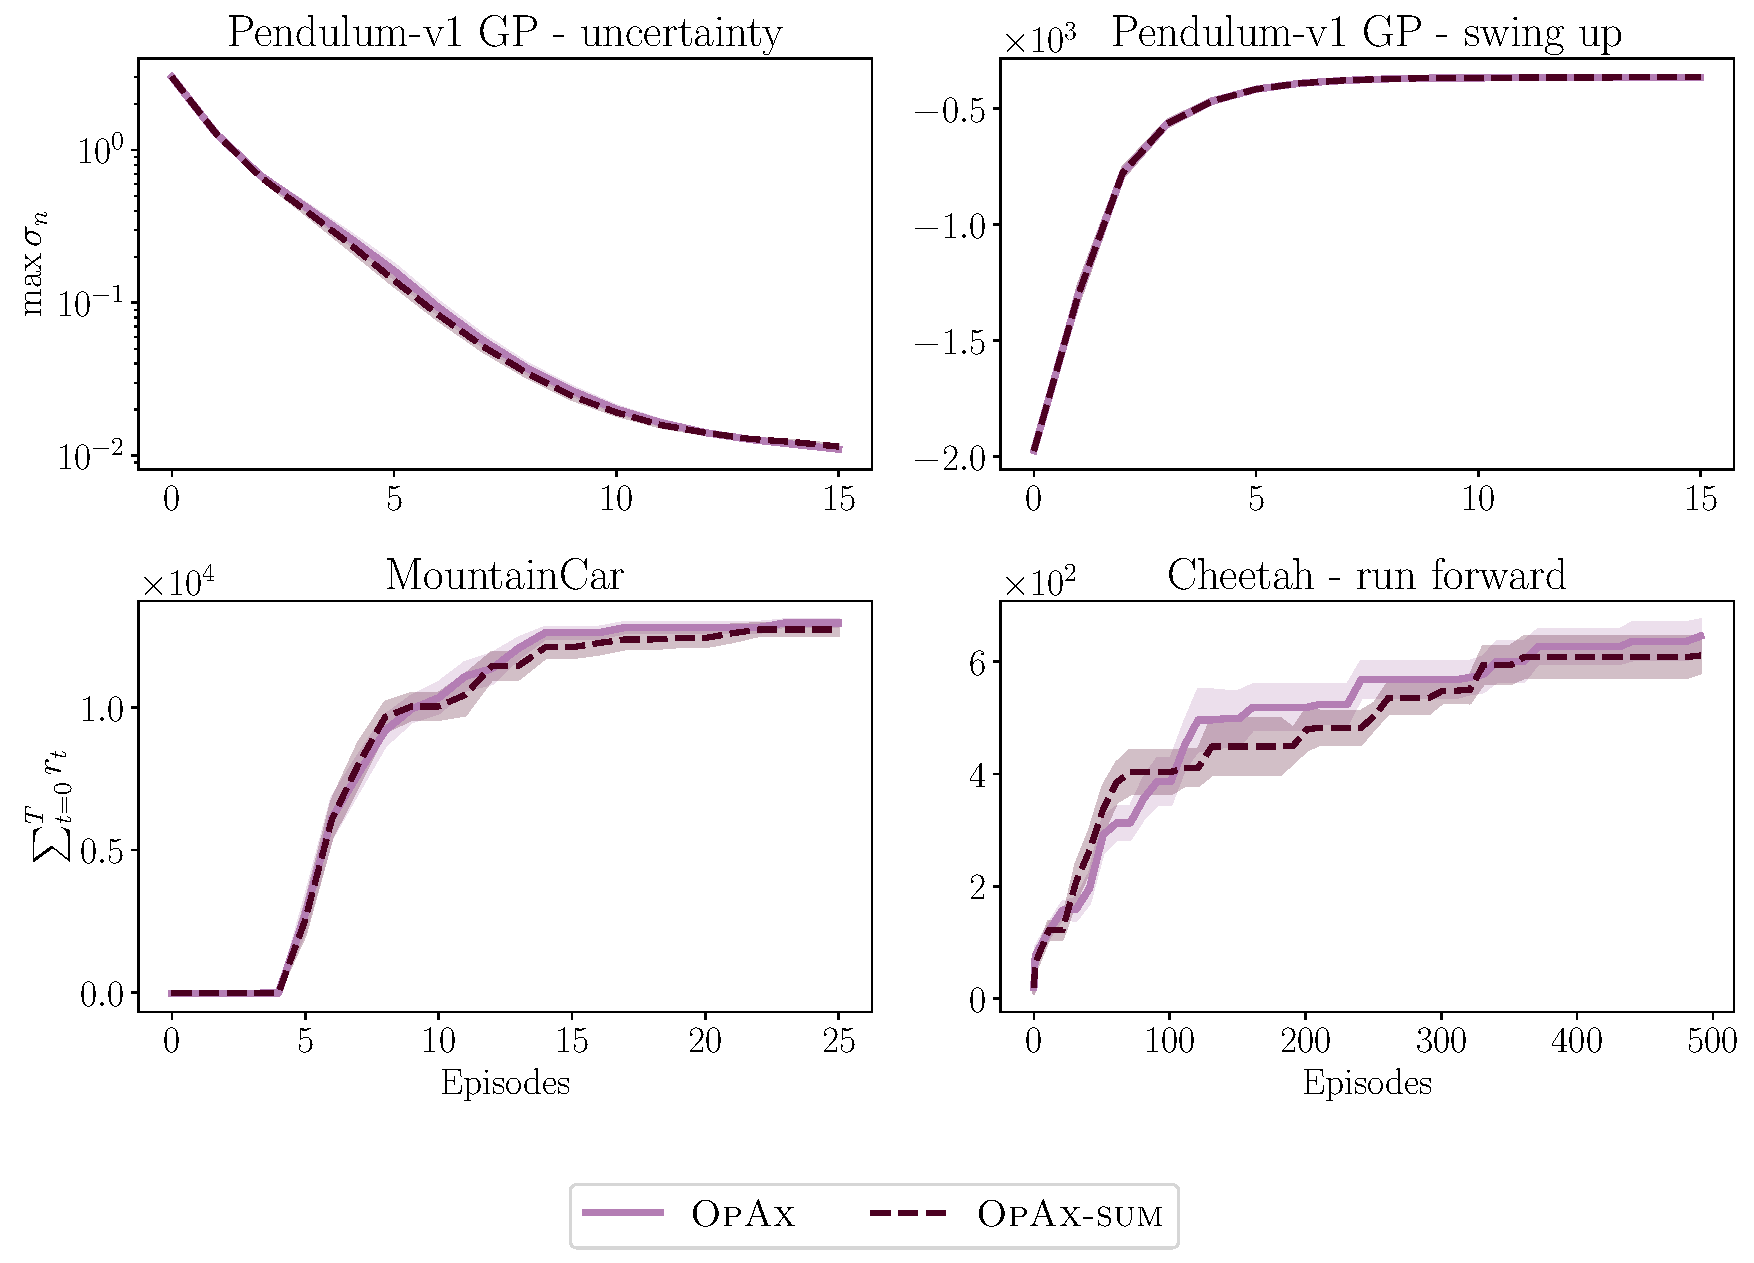
\includegraphics[width=0.8\textwidth]{figures/sum_rewards_comparison.pdf}
    \caption{Comparison of \opacex between intrinsic reward proposed in \Cref{eq:exploration_op} and the sum of epistemic uncertainties proposed by~\citep{pathak2019self}, i.e., \opacex-\textsc{sum}. For both choices of intrinsic rewards, \opacex reduces the epistemic uncertainty and performs well on downstream tasks.}
    \label{fig:comparison_sum}
\end{figure}
The intrinsic reward suggested in \Cref{eq:exploration_op} takes the log of the model epistemic uncertainty. Another common choice for the intrinsic reward is the epistemic uncertainty or model disagreement without the log~\citep{pathak2019self, sekar2020planning}. In the following Lemma, we show that these rewards are closely related.
\begin{lemma}
    Let  $\sigma_{\max} = \sup_{\vz \in \setZ; i \geq 0; 1\leq j\leq d_x} \sigma_{i, j}(\vz)$ and $\sigma >  0$. Then for all $i\geq 0$ and $j \in \{1, \dots, d_x\}$
    \begin{equation*}
        \sigma^2_{i, j}(\vz) \leq \frac{\sigma_{\max}}{\log(1 + \sigma^{-2}\sigma_{\max})}\log(1 + \sigma^{-2}\sigma^2_{i, j}(\vz)) \leq \frac{\sigma^{-2}\sigma_{\max}}{\log(1 + \sigma^{-2}\sigma_{\max})} \sigma^2_{i, j}(\vz). 
    \end{equation*}
\end{lemma}
\begin{proof}
\cite{curi2020efficient}  derive the first inequality on the left. The second inequality follows since $\log(1 + x) \leq x$ for all $x \geq 0$.
\end{proof}
\looseness=-1
Due to this close relation between the two objectives, our theoretical findings also apply to the intrinsic reward proposed by~\citep{pathak2019self}. Moreover, empirically we notice in~\Cref{fig:comparison_sum} that \opacex performs similarly when the sum of epistemic uncertainties is used instead of the objective in \Cref{eq:exploration_op}. However, our objective can naturally be extended to the case of heteroscedastic aleatoric noise, since it trades off the ratio of epistemic and aleatoric uncertainty.

\begin{comment}
\section{Submission of papers to NeurIPS 2023}


Please read the instructions below carefully and follow them faithfully. \textbf{Important:} This year the checklist will be submitted separately from the main paper in OpenReview, please review it well ahead of the submission deadline: \url{https://neurips.cc/public/guides/PaperChecklist}.


\subsection{Style}


Papers to be submitted to NeurIPS 2023 must be prepared according to the
instructions presented here. Papers may only be up to {\bf nine} pages long,
including figures. Additional pages \emph{containing only acknowledgments and
references} are allowed. Papers that exceed the page limit will not be
reviewed, or in any other way considered for presentation at the conference.


The margins in 2023 are the same as those in previous years.


Authors are required to use the NeurIPS \LaTeX{} style files obtainable at the
NeurIPS website as indicated below. Please make sure you use the current files
and not previous versions. Tweaking the style files may be grounds for
rejection.


\subsection{Retrieval of style files}


The style files for NeurIPS and other conference information are available on
the website at
\begin{center}
  \url{http://www.neurips.cc/}
\end{center}
The file \verb+neurips_2023.pdf+ contains these instructions and illustrates the
various formatting requirements your NeurIPS paper must satisfy.


The only supported style file for NeurIPS 2023 is \verb+neurips_2023.sty+,
rewritten for \LaTeXe{}.  \textbf{Previous style files for \LaTeX{} 2.09,
  Microsoft Word, and RTF are no longer supported!}


The \LaTeX{} style file contains three optional arguments: \verb+final+, which
creates a camera-ready copy, \verb+preprint+, which creates a preprint for
submission to, e.g., arXiv, and \verb+nonatbib+, which will not load the
\verb+natbib+ package for you in case of package clash.


\paragraph{Preprint option}
If you wish to post a preprint of your work online, e.g., on arXiv, using the
NeurIPS style, please use the \verb+preprint+ option. This will create a
nonanonymized version of your work with the text ``Preprint. Work in progress.''
in the footer. This version may be distributed as you see fit, as long as you do not say which conference it was submitted to. Please \textbf{do
  not} use the \verb+final+ option, which should \textbf{only} be used for
papers accepted to NeurIPS. 


At submission time, please omit the \verb+final+ and \verb+preprint+
options. This will anonymize your submission and add line numbers to aid
review. Please do \emph{not} refer to these line numbers in your paper as they
will be removed during generation of camera-ready copies.


The file \verb+neurips_2023.tex+ may be used as a ``shell'' for writing your
paper. All you have to do is replace the author, title, abstract, and text of
the paper with your own.


The formatting instructions contained in these style files are summarized in
Sections \ref{gen_inst}, \ref{headings}, and \ref{others} below.


\section{Problem Setting}
\label{problem_setting}
In this work, we study a discrete-time dynamical system $f^*$.


The paper title should be 17~point, initial caps/lower case, bold, centered
between two horizontal rules. The top rule should be 4~points thick and the
bottom rule should be 1~point thick. Allow \nicefrac{1}{4}~inch space above and
below the title to rules. All pages should start at 1~inch (6~picas) from the
top of the page.


For the final version, authors' names are set in boldface, and each name is
centered above the corresponding address. The lead author's name is to be listed
first (left-most), and the co-authors' names (if different address) are set to
follow. If there is only one co-author, list both author and co-author side by
side.


Please pay special attention to the instructions in Section \ref{others}
regarding figures, tables, acknowledgments, and references.


\section{Headings: first level}
\label{headings}


All headings should be lower case (except for first word and proper nouns),
flush left, and bold.


First-level headings should be in 12-point type.


\subsection{Headings: second level}


Second-level headings should be in 10-point type.


\subsubsection{Headings: third level}


Third-level headings should be in 10-point type.


\paragraph{Paragraphs}


There is also a \verb+\paragraph+ command available, which sets the heading in
bold, flush left, and inline with the text, with the heading followed by 1\,em
of space.


\section{Citations, figures, tables, references}
\label{others}


These instructions apply to everyone.


\subsection{Citations within the text}


The \verb+natbib+ package will be loaded for you by default.  Citations may be
author/year or numeric, as long as you maintain internal consistency.  As to the
format of the references themselves, any style is acceptable as long as it is
used consistently.


The documentation for \verb+natbib+ may be found at
\begin{center}
  \url{http://mirrors.ctan.org/macros/latex/contrib/natbib/natnotes.pdf}
\end{center}
Of note is the command \verb+\citet+, which produces citations appropriate for
use in inline text.  For example,
\begin{verbatim}
   \citet{hasselmo} investigated\dots
\end{verbatim}
produces
\begin{quote}
  Hasselmo, et al.\ (1995) investigated\dots
\end{quote}


If you wish to load the \verb+natbib+ package with options, you may add the
following before loading the \verb+neurips_2023+ package:
\begin{verbatim}
   \PassOptionsToPackage{options}{natbib}
\end{verbatim}


If \verb+natbib+ clashes with another package you load, you can add the optional
argument \verb+nonatbib+ when loading the style file:
\begin{verbatim}
   \usepackage[nonatbib]{neurips_2023}
\end{verbatim}


As submission is double blind, refer to your own published work in the third
person. That is, use ``In the previous work of Jones et al.\ [4],'' not ``In our
previous work [4].'' If you cite your other papers that are not widely available
(e.g., a journal paper under review), use anonymous author names in the
citation, e.g., an author of the form ``A.\ Anonymous'' and include a copy of the anonymized paper in the supplementary material.


\subsection{Footnotes}


Footnotes should be used sparingly.  If you do require a footnote, indicate
footnotes with a number\footnote{Sample of the first footnote.} in the
text. Place the footnotes at the bottom of the page on which they appear.
Precede the footnote with a horizontal rule of 2~inches (12~picas).


Note that footnotes are properly typeset \emph{after} punctuation
marks.\footnote{As in this example.}


\subsection{Figures}


\begin{figure}
  \centering
  \fbox{\rule[-.5cm]{0cm}{4cm} \rule[-.5cm]{4cm}{0cm}}
  \caption{Sample figure caption.}
\end{figure}


All artwork must be neat, clean, and legible. Lines should be dark enough for
purposes of reproduction. The figure number and caption always appear after the
figure. Place one line space before the figure caption and one line space after
the figure. The figure caption should be lower case (except for first word and
proper nouns); figures are numbered consecutively.


You may use color figures.  However, it is best for the figure captions and the
paper body to be legible if the paper is printed in either black/white or in
color.


\subsection{Tables}


All tables must be centered, neat, clean and legible.  The table number and
title always appear before the table.  See Table~\ref{sample-table}.


Place one line space before the table title, one line space after the
table title, and one line space after the table. The table title must
be lower case (except for first word and proper nouns); tables are
numbered consecutively.


Note that publication-quality tables \emph{do not contain vertical rules.} We
strongly suggest the use of the \verb+booktabs+ package, which allows for
typesetting high-quality, professional tables:
\begin{center}
  \url{https://www.ctan.org/pkg/booktabs}
\end{center}
This package was used to typeset Table~\ref{sample-table}.


\begin{table}
  \caption{Sample table title}
  \label{sample-table}
  \centering
  \begin{tabular}{lll}
    \toprule
    \multicolumn{2}{c}{Part}                   \\
    \cmidrule(r){1-2}
    Name     & Description     & Size ($\mu$m) \\
    \midrule
    Dendrite & Input terminal  & $\sim$100     \\
    Axon     & Output terminal & $\sim$10      \\
    Soma     & Cell body       & up to $10^6$  \\
    \bottomrule
  \end{tabular}
\end{table}

\subsection{Math}
Note that display math in bare TeX commands will not create correct line numbers for submission. Please use LaTeX (or AMSTeX) commands for unnumbered display math. (You really shouldn't be using \$\$ anyway; see \url{https://tex.stackexchange.com/questions/503/why-is-preferable-to} and \url{https://tex.stackexchange.com/questions/40492/what-are-the-differences-between-align-equation-and-displaymath} for more information.)

\subsection{Final instructions}

Do not change any aspects of the formatting parameters in the style files.  In
particular, do not modify the width or length of the rectangle the text should
fit into, and do not change font sizes (except perhaps in the
\textbf{References} section; see below). Please note that pages should be
numbered.


\section{Preparing PDF files}


Please prepare submission files with paper size ``US Letter,'' and not, for
example, ``A4.''


Fonts were the main cause of problems in the past years. Your PDF file must only
contain Type 1 or Embedded TrueType fonts. Here are a few instructions to
achieve this.


\begin{itemize}


\item You should directly generate PDF files using \verb+pdflatex+.


\item You can check which fonts a PDF files uses.  In Acrobat Reader, select the
  menu Files$>$Document Properties$>$Fonts and select Show All Fonts. You can
  also use the program \verb+pdffonts+ which comes with \verb+xpdf+ and is
  available out-of-the-box on most Linux machines.


\item \verb+xfig+ "patterned" shapes are implemented with bitmap fonts.  Use
  "solid" shapes instead.


\item The \verb+\bbold+ package almost always uses bitmap fonts.  You should use
  the equivalent AMS Fonts:
\begin{verbatim}
   \usepackage{amsfonts}
\end{verbatim}
followed by, e.g., \verb+\mathbb{R}+, \verb+\mathbb{N}+, or \verb+\mathbb{C}+
for $\mathbb{R}$, $\mathbb{N}$ or $\mathbb{C}$.  You can also use the following
workaround for reals, natural and complex:
\begin{verbatim}
   \newcommand{\RR}{I\!\!R} %real numbers
   \newcommand{\Nat}{I\!\!N} %natural numbers
   \newcommand{\CC}{I\!\!\!\!C} %complex numbers
\end{verbatim}
Note that \verb+amsfonts+ is automatically loaded by the \verb+amssymb+ package.


\end{itemize}


If your file contains type 3 fonts or non embedded TrueType fonts, we will ask
you to fix it.


\subsection{Margins in \LaTeX{}}


Most of the margin problems come from figures positioned by hand using
\verb+\special+ or other commands. We suggest using the command
\verb+\includegraphics+ from the \verb+graphicx+ package. Always specify the
figure width as a multiple of the line width as in the example below:
\begin{verbatim}
   \usepackage[pdftex]{graphicx} ...
   \includegraphics[width=0.8\linewidth]{myfile.pdf}
\end{verbatim}
See Section 4.4 in the graphics bundle documentation
(\url{http://mirrors.ctan.org/macros/latex/required/graphics/grfguide.pdf})


A number of width problems arise when \LaTeX{} cannot properly hyphenate a
line. Please give LaTeX hyphenation hints using the \verb+\-+ command when
necessary.


\begin{ack}
Use unnumbered first level headings for the acknowledgments. All acknowledgments
go at the end of the paper before the list of references. Moreover, you are required to declare
funding (financial activities supporting the submitted work) and competing interests (related financial activities outside the submitted work).
More information about this disclosure can be found at: \url{https://neurips.cc/Conferences/2023/PaperInformation/FundingDisclosure}.


Do {\bf not} include this section in the anonymized submission, only in the final paper. You can use the \texttt{ack} environment provided in the style file to autmoatically hide this section in the anonymized submission.
\end{ack}



\section{Supplementary Material}

Authors may wish to optionally include extra information (complete proofs, additional experiments and plots) in the appendix. All such materials should be part of the supplemental material (submitted separately) and should NOT be included in the main submission.


\section*{References}


References follow the acknowledgments in the camera-ready paper. Use unnumbered first-level heading for
the references. Any choice of citation style is acceptable as long as you are
consistent. It is permissible to reduce the font size to \verb+small+ (9 point)
when listing the references.
Note that the Reference section does not count towards the page limit.
\medskip


{
\small


[1] Alexander, J.A.\ \& Mozer, M.C.\ (1995) Template-based algorithms for
connectionist rule extraction. In G.\ Tesauro, D.S.\ Touretzky and T.K.\ Leen
(eds.), {\it Advances in Neural Information Processing Systems 7},
pp.\ 609--616. Cambridge, MA: MIT Press.


[2] Bower, J.M.\ \& Beeman, D.\ (1995) {\it The Book of GENESIS: Exploring
  Realistic Neural Models with the GEneral NEural SImulation System.}  New York:
TELOS/Springer--Verlag.


[3] Hasselmo, M.E., Schnell, E.\ \& Barkai, E.\ (1995) Dynamics of learning and
recall at excitatory recurrent synapses and cholinergic modulation in rat
hippocampal region CA3. {\it Journal of Neuroscience} {\bf 15}(7):5249-5262.
}

%%%%%%%%%%%%%%%%%%%%%%%%%%%%%%%%%%%%%%%%%%%%%%%%%%%%%%%%%%%%
\end{comment}

\end{document}